\pdfinfoomitdate=1
\documentclass[11pt]{article}
\usepackage[T1]{fontenc}
\usepackage{lmodern}
\usepackage[margin=1in]{geometry}
\usepackage{amsmath,amssymb,amsthm,mathtools}
\usepackage{microtype}
\usepackage{enumitem,booktabs,longtable}
\usepackage{graphicx,tikz}
\usetikzlibrary{arrows.meta,positioning,calc,patterns,fit,backgrounds}
\usepackage[numbers,sort&compress]{natbib}
\usepackage[hidelinks]{hyperref}
\usepackage[capitalise,nameinlink,noabbrev]{cleveref}
\makeatletter
\newcommand{\psc@thmrefstepcounter}[2][]{%
  \let\psc@saved@refstepcounter\cref@old@refstepcounter
  \let\cref@old@refstepcounter\Hy@theorem@refstepcounter
  \refstepcounter[#1]{#2}%
  \let\cref@old@refstepcounter\psc@saved@refstepcounter
}
\patchcmd{\cref@thmoptarg}{\refstepcounter}{\psc@thmrefstepcounter}{}
  {\PackageError{psc-width}{Shared-counter theorem patch failed}%
    {The installed cleveref/hyperref combination needs a compatibility review.}}
\patchcmd{\cref@thmnoarg}{\refstepcounter}{\Hy@theorem@refstepcounter}{}
  {\PackageError{psc-width}{Base-counter theorem patch failed}%
    {The installed cleveref/hyperref combination needs a compatibility review.}}
\makeatother
\setlength{\emergencystretch}{2em}
\setlist{itemsep=3pt,topsep=5pt}
\numberwithin{equation}{section}
\newtheorem{theorem}{Theorem}[section]
\newtheorem{lemma}[theorem]{Lemma}
\newtheorem{proposition}[theorem]{Proposition}
\newtheorem{corollary}[theorem]{Corollary}
\theoremstyle{definition}
\newtheorem{definition}[theorem]{Definition}
\newtheorem{convention}[theorem]{Convention}
\theoremstyle{remark}
\newtheorem{remark}[theorem]{Remark}
\newcommand{\R}{\mathbb R}
\newcommand{\N}{\mathbb N}
\newcommand{\Z}{\mathbb Z}
\newcommand{\T}{\mathbb T}
\newcommand{\Fcal}{\mathcal F}
\newcommand{\dd}{\mathrm d}
\newcommand{\eps}{\varepsilon}
\DeclareMathOperator{\Scal}{Scal}
\DeclareMathOperator{\Div}{div}
\DeclareMathOperator{\grad}{grad}
\DeclareMathOperator{\lap}{\Delta}
\DeclareMathOperator{\supp}{supp}
\DeclareMathOperator{\dist}{dist}
\DeclareMathOperator{\diam}{diam}
\DeclareMathOperator{\vol}{vol}
\DeclareMathOperator{\tr}{tr}
\DeclareMathOperator{\Ric}{Ric}
\DeclareMathOperator{\Hess}{Hess}
\DeclareMathOperator{\Id}{Id}
\DeclareMathOperator{\UW}{UW}
\DeclarePairedDelimiter{\abs}{\lvert}{\rvert}
\DeclarePairedDelimiter{\norm}{\lVert}{\rVert}
\title{Positive scalar curvature and uniform codimension-two width}
\author{OpenAI}
\date{September 23, 2026}
\hypersetup{pdftitle={Positive scalar curvature and uniform codimension-two width},pdfauthor={OpenAI}}
\begin{document}
\maketitle
\begin{abstract}
We prove the quantitative continuous form of Gromov's scalar-curvature
conjecture in every dimension $n\ge4$. Every complete connected smooth
boundaryless $n$-manifold with scalar curvature at least one admits a
continuous map to a simplicial complex of dimension at most $n-2$ whose
entire fibers have diameter bounded only in terms of $n$. We also obtain
the continuous macroscopic-dimension conclusion for
universal covers of closed manifolds with positive scalar curvature in
every dimension $n\ge2$.
\end{abstract}
\begingroup\small\tableofcontents\endgroup
\clearpage
\section{Introduction}\label{sec:introduction}

A lower bound for scalar curvature is a local condition. Gromov's
macroscopic dimension conjecture predicts a global consequence: at a
controlled scale, two dimensions can be collapsed. We prove the
quantitative form of this assertion for arbitrary complete manifolds
in dimensions at least four.

Throughout, scalar curvature means the ordinary pointwise Riemannian
invariant. Fixed-scale macroscopic scalar curvature uses ball-volume
comparison at a prescribed positive radius
\citep[Definitions~1.2--1.3]{kumarSen2026Width}.

For a metric space \(X\) and an integer \(d\ge0\), define its
\emph{Urysohn \(d\)-width} by
\[
 \UW_d(X)=\inf_f\ \sup_{y\in K}\diam_X f^{-1}(y),
\]
where the infimum runs over continuous maps \(f:X\to K\) to simplicial
complexes of dimension at most \(d\). The complexes have their usual
polyhedral topology. The diameter is that of the entire fiber, including
all its components; empty fibers may be omitted.

\begin{theorem}\label{thm:main}
For every integer \(n\ge4\), there is a finite constant \(C_n\) such
that every connected complete smooth Riemannian \(n\)-manifold
\((M,g)\), without boundary and with \(\Scal_g\ge1\), admits a
continuous map \(f:M\to K\) to a simplicial complex of dimension at
most \(n-2\) satisfying
\[
 \diam_g f^{-1}(y)\le C_n\qquad(y\in K).
\]
In particular, \(\UW_{n-2}(M,g)\le C_n\).
\end{theorem}

The constant is independent of \(M\), its topology, and its geometry.
The theorem applies to compact and noncompact manifolds, with no
orientability, spin, covering, or bounded geometry assumption. If
\(\Scal_g\ge\sigma^2>0\), applying the theorem to \(\sigma^2g\) gives
\(\UW_{n-2}(M,g)\le C_n/\sigma\).

For a closed connected Riemannian manifold, let
\(\operatorname{FillRad}(M,g)\) be Gromov's filling radius
\citep{gromov1983Filling}, defined by the Kuratowski embedding and the
fundamental class, with coefficients in
\(\Z\) if \(M\) is orientable and in \(\Z_2\) otherwise
\citep[Definition~3.1]{nabutovskyRotmanSabourau2021}.
The next corollary gives the closed-manifold case in dimensions at least
four of Gromov's filling-radius Conjecture~\(A^{-}\)
\citep[\S3]{gromov2017Dozen}.

\begin{corollary}[Closed-manifold filling-radius bound]
\label{cor:filling-radius}
Let \((M,g)\) be a closed connected smooth Riemannian \(n\)-manifold
with \(n\ge4\) and \(\Scal_g\ge\sigma^2\) for some \(\sigma>0\). Then
\[
 \operatorname{FillRad}(M,g)\le \frac{C_n}{2\sigma},
\]
where \(C_n\) is the constant in Theorem~\ref{thm:main}.
\end{corollary}

\begin{proof}
Gromov's comparison, in the form recorded by Nabutovsky, Rotman, and
Sabourau \citep[Definition~6.1 and equation~(6.1)]{nabutovskyRotmanSabourau2021},
uses the same continuous-map and entire-fiber width convention as above.
A target of dimension at most \(n-2\) is also admissible for
\(\UW_{n-1}\). Since \(M\) is closed, the comparison and the scaled
form of Theorem~\ref{thm:main} give
\[
 \operatorname{FillRad}(M,g)
 \le \tfrac12\UW_{n-1}(M,g)
 \le \tfrac12\UW_{n-2}(M,g)
 \le \frac{C_n}{2\sigma}.
\]
\end{proof}

For the closed-cover consequence we also use the \emph{continuous
macroscopic dimension}: $\dim_{\mathrm{mc}}X\le d$ means that there is a
continuous map to a simplicial complex of dimension at most $d$, with its uniform simplex metric
and a finite uniform bound on the diameters of its entire fibers.
Each simplex has the same standard Euclidean shape and edge length.

\begin{corollary}[Continuous macroscopic dimension of universal covers]
\label{cover:main}
Let $(M,h)$ be a closed connected smooth Riemannian manifold of
dimension $n\ge2$ with positive scalar curvature.  Its universal cover,
with the lifted original metric $\widetilde h$, satisfies
\[
 \dim_{\mathrm{mc}}(\widetilde M,\widetilde h)\le n-2.
\]
\end{corollary}

\begin{corollary}[Aspherical obstruction]\label{cor:aspherical}
No closed smooth aspherical manifold of dimension \(n\ge4\) admits
a Riemannian metric of strictly positive scalar curvature.
\end{corollary}

\begin{proof}
It suffices to consider a connected manifold; passing to its orientation
double cover if necessary preserves the hypotheses. Suppose such a metric
exists. Its scalar curvature has a positive minimum, so the lifted metric
on the contractible universal cover \(X\) is complete with a uniform
positive scalar-curvature lower bound. The deck group acts isometrically
and cocompactly. The scaled form of Theorem~\ref{thm:main} gives a
continuous map from \(X\) to an \((n-2)\)-complex with uniformly bounded
entire fibers. The width and filling-radius implications in Gromov's
noncompact argument \(A^+\Rightarrow B\)
\citep[\S3, pp.~6--8]{gromov2017Dozen} exclude such a map on a
contractible universal cover with a cocompact deck action. This gives
the contradiction.
\end{proof}

An independent proof in every dimension follows from the stronger
rational-inessentiality theorem of
\citet[Theorem~1.1 and Corollary~1.2]{openai2026RationalInessentiality}.

\subsection{History and significance}

Gromov introduced macroscopic dimension in his study of positive scalar
curvature \citep[\S2]{gromov1996}. His quantitative conjecture already asks
whether a complete manifold with a positive scalar-curvature lower bound
can be mapped continuously to a polyhedron of codimension two with all
point inverses bounded at the curvature scale
\citep[\S\(2\frac12\)]{gromov1996}; see also
\citep[p.~3180, Comments after Conjecture~3.2]{gromov2019Mean}.
The diameter condition concerns each entire fiber, including all its
components. In the universal cover of a closed manifold the corresponding
macroscopic-dimension assertion asks only for some finite bound.
The continuous invariant and the version requiring a Lipschitz map to a
uniformly metrized complex are distinct
\citep[Definitions~1.1--1.2]{dranishnikov2014}.

The pointwise curvature hypothesis cannot be replaced by its fixed-scale
macroscopic counterpart. Kumar and Sen construct closed manifolds in
every dimension at least four with a prescribed positive fixed-scale
macroscopic scalar-curvature lower bound and arbitrarily large
Urysohn codimension-two width \citep[Theorem~A]{kumarSen2026Width}.

The low-dimensional cases have a substantial earlier history.
Gromov and Lawson obtained geometric width bounds for closed three-manifolds
\citep[Corollary~10.11]{gromovLawson1983}, and Bolotov proved that the
universal cover of a closed three-manifold cannot have macroscopic
dimension two \citep{bolotov2003}.
For closed three-manifolds with positive scalar curvature, Liokumovich
and Maximo constructed Morse functions with curvature-scale bounds for
the areas and ambient diameters of connected level components
\citep[Theorem~1.1]{liokumovichMaximo2023}.
Liokumovich and Wang constructed proper Morse functions on
complete noncompact three-manifolds with uniformly positive scalar
curvature, with uniform diameter bounds for connected level components
\citep[Theorem~1.1]{liokumovichWang2023}.
We use that result and an explicit passage to the Reeb graph for the
three-dimensional closed-cover consequence; the surface case follows
from the Bonnet--Myers argument.

The aspherical obstruction in dimensions four and five was established
by Chodosh and Li \citep[Theorem~2]{chodoshLi}, with an independent
proof in dimension five by Gromov
\citep[\S7, Main Corollary]{gromov2020Aspherical}.

For the macroscopic-dimension conjecture, Bolotov proved the closed spin
case under the Strong Novikov Conjecture and a cohomological-dimension condition
\citep{bolotov2009}. Bolotov and Dranishnikov then obtained the
codimension-two conclusion for closed spin manifolds under the
Strong Novikov Conjecture and
injectivity of the connective-to-periodic real K-homology map
\citep[Theorem~4.3]{bolotovDranishnikov2010}.
For closed orientable totally non-spin manifolds of dimension at least
five, they also showed that a macroscopic dimension drop by one implies
a drop by two \citep[Theorem~3.4]{bolotovDranishnikov2016}.
Daher and Dranishnikov established the analogous implication for closed
orientable totally non-spin four-manifolds with residually finite
fundamental group
\citep[Theorem~3.3]{daherDranishnikov2019}.
These topological advances concern universal covers and finite bounds;
the present quantitative statement is formulated for arbitrary complete
manifolds with a bound depending only on dimension after scalar normalization.


The geometric method uses the minimal-hypersurface approach of Schoen
and Yau, in which stability and the Gauss equation pass scalar-curvature
information to hypersurfaces \citep[Section~1]{schoenYau1979Structure},
and the torical symmetrization mechanism described by Gromov
\citep[Section~2]{gromov2018Metric}. Gromov's \(\mu\)-bubble method
uses prescribed mean curvature to localize the hypersurfaces entering
scalar-curvature descent \citep[\S\(5\frac56\)]{gromov1996}.
The weighted variational formulation and its relation to warped-circle
geometry and stability are developed by Chodosh and Li
\citep[Section~3 and Remark~11]{chodoshLi}.

Removing singular regions while retaining scalar-curvature information
is also central to Lohkamp's splitting theory
\citep[\S1.2 and Theorem~3.15]{lohkamp2022SplittingsII}.
In the construction below, profile updates exclude singular points from
the regions where the next scalar bound is required; the wall and both
retained sides are then regularized together.

Recent results also address quantitative width and singular descent.
Antonelli proves width bounds under a positive scalar-curvature lower
bound, an almost-nonnegative Ricci lower bound, and uniform noncollapse,
with constants depending on the volume lower bound
\citep[Theorem~1.4]{antonelli2026Volume}.
Bi and Zhu develop singular scalar-curvature descent for enlargeability
obstructions and cubical-width inequalities
\citep[Theorem~B and Section~4]{biZhu2026}.
The present construction retains both bulk sides and the wall through
countably many cuts, with compatible product ends.

\subsection{The proof and its main constructions}

Fix an original length \(D\), depending only on \(n\), and a separated
net \((x_i)\) in \((M,g)\). The inner balls of radius \(D\) cover \(M\),
and the closed outer balls of radius \(2D\) are locally finite. Each
center has its own label. We construct a continuous collapse map
$q:M\to M$ with $d_g(q(x),x)<1$, together with compatible walls
separating the inverse images of each inner ball and the exterior of
its outer ball. The map $q$ records original positions while cylinders
are inserted along the cuts. The final
walls have no common intersection of \(n-1\) distinct labels. Continuous
sign coordinates $t_i:M\to[0,1]$ are chosen to equal $1$ on the
$q$-preimage of the inner ball and $0$ on the $q$-preimage of the exterior
of its outer ball. Their transition regions lie in wall neighborhoods
chosen simultaneously to preserve the intersection bound. They give the
desired map: at most \(n-2\) coordinates
are fractional at a point, and some coordinate is one. Equality of all
coordinates confines both collapse images to the same original outer
ball, giving a bound for the entire fiber.

Three points are essential to make this construction uniform and to
allow arbitrary complete metrics.

First, the separations must become as wide as prescribed without
spending curvature in proportion to the number of labels. For a metric
\(h\) and a smooth function \(t\), put
\begin{equation}\label{intro:drift-scalar}
 \mathcal D(h,t)=\Scal_h+2\Delta_h t-|\dd t|_h^2.
\end{equation}
Fix a background metric \(h_0\) throughout a round. The local stretching
estimate changes \(h\) monotonically and increases \(t\), while paying
for its loss with a decrease in \(\tr_h h_0\).
The pressure law in \Cref{pressure:law} provides a quadratic budget in
\(t\). This makes the initial scale depend only on \(n\), even when
there is no bound on the overlap multiplicity of the original balls.
Trace losses telescope over a countable locally finite round. Each
label stops after its own finite number of rounds, so the entire
construction stabilizes on every compact set
(\Cref{rounds:wide}). Diagonal circle warps convert the drift scalar
bound to an ordinary scalar-curvature inequality on every required
finite product.

Second, a cut produces both extended bulk sides and a wall of one lower
base dimension. We keep all these pieces, called \emph{packets}, with
compatible product collars. Each label has two open \emph{forced cores},
one of each sign, on which that sign must be retained. A label is
\emph{decided} at a point when the point lies in one of its cores.
On an \(m\)-dimensional packet, positive
scalar curvature is required only where at least \(m-1\) remaining
labels are outside their forced cores. Minimizing walls may be
singular in high dimensions. Near the dangerous singular region,
additional pressure profiles make the remaining labels decided.
Hardy estimates, compactness across the bulk--cylinder seam, and a
maximum estimate for concentrating potentials pay for this shielding.
A guarded regularization and positive supersolutions then restore
smooth scalar-curvature control. The full finite-diagram arguments are
proved in \Cref{sec:packets,sec:cut,sec:local,sec:shield-global,sec:regularization}.
They include the stability and variation computations used here;
classical elliptic and geometric-measure-theory results are cited with
their hypotheses at their points of use.

Third, a countable list needs more than finiteness on compact subsets.
After a first radial cut, only finitely many labels and warp factors
are nonconstant on any \emph{whole} packet and on each finite incident
diagram needed by a step. All other labels are already forced; their
potentials form a summable list of spatial constants. Approximations
reproduce those constants exactly. This invariant permits the finite
packet arguments to be iterated with successively smaller positive
budgets, without a common positive floor for all labels. An intersection
of \(n-1\) distinct walls would produce a complete one-dimensional
packet. The positive scalar-curvature invariant on its finite warped
product yields a Riccati inequality that cannot hold on the complete
arclength line (\Cref{countable:dimension-one}), giving the required
wall-intersection bound.

Finally, the analytic cylinders are used only through finite
truncations in the topological reconstruction. Successive collar
compressions are supported over the corresponding original outer
balls. On one fixed copy of \(M\), the collapse maps and the old wall
statuses are therefore eventually unchanged near every point. This
local stabilization, together with a locally finite thickening of the
walls, gives continuity in the ordinary polyhedral topology. The
resulting constant is
\[
 C_n=4D+2,
\]
where the original scale \(D\) is chosen in terms of \(n\) before any
metric-dependent analytic estimates. The construction does not aim to optimize this constant.

The proof follows two separate inputs. Sections~\ref{pressure:section}--\ref{sec:rounds}
construct the geometric stretching and its scalar reserve.
Section~\ref{sec:finite-cuts} states the finite-label cutting procedure,
whose complete proof occupies Appendices~\ref{sec:packets}--\ref{sec:regularization}.
Section~\ref{sec:countable} proves its countable-label adaptation, and
Section~\ref{sec:reconstruction} constructs the width map.
Section~\ref{sec:closed-covers} verifies the uniform simplex metric and
proves the closed-cover consequence in dimensions two and three.

\begin{convention}\label{conv:signs}
The Laplacian is \(\Delta=\Div\grad\), and round spheres have positive
scalar curvature. For a hypersurface with unit normal \(\nu\), its
second fundamental form is
\(B(v,w)=\langle\nabla_v\nu,w\rangle\), and its mean curvature is
\(\tr B\). Integration and divergence use Riemannian densities, so no
orientation is needed. Distances in the final fiber bound are always
measured in the original metric \(g\).
\end{convention}

\section{A pressure law with a quadratic budget}
\label{pressure:section}

The local metric deformation will use a pressure depending both on a height
variable $x$ and on the drift parameter $t$.  Its derivative in $x$ must be
large, while a large positive derivative in $x$ must be accompanied by a
favorable derivative in $t$.  The following construction supplies these
properties with constants chosen before any local geometric data.

\begin{theorem}[Pressure law]\label{pressure:law}
For every $A_0,P_0,\eps,b_0>0$ there exist $0<S_0\le1$, $T\ge1$, and a
smooth function
\[
 F:(-S_0,S_0)\times[T,\infty)\longrightarrow\R
\]
which is odd in $x$, has $F_x>0$, and satisfies
\begin{equation}\label{pressure:estimates}
\begin{gathered}
 F_x\ge A_0t,\qquad |F_t|\le\eps|F|,\qquad FF_t\le\eps F_x,\\
 F_x\le b_0t^2\quad\text{or}\quad -FF_t\ge P_0F_x,\\
 F_x\le b_0t^2+\eps F^2.
\end{gathered}
\end{equation}
For each fixed $t\ge T$,
\[
 \lim_{x\to-S_0}F(x,t)=-\infty,
 \qquad \lim_{x\to S_0}F(x,t)=+\infty.
\]
These limits are uniform when $t$ ranges over a compact subinterval of
$[T,\infty)$.  The choices depend only on $A_0,P_0,\eps,b_0$ and fixed
numerical constants.  In particular, they are independent of any manifold,
metric, local cutoff, or subsequent deformation parameter.  The lower bound
$T$ may be increased after the construction.
\end{theorem}

\begin{proof}
We construct $F$ by prescribing its inverse in the first variable. For
the moment, let $k>0$ and let $g$ be a positive smooth function on
$[0,\infty)$, both to be chosen. Write $f>0$ for an independent pressure
value and, for $t>0$, set
\begin{equation}\label{pressure:inverse}
 X(f,t)=\frac1k\arctan\frac{f^{1/3}}{g(y)},\qquad
 q=f^{2/3},\qquad y=\frac tq.
\end{equation}
Put $A(y)=g(y)+2yg'(y)$. Differentiation at fixed $f$ or at fixed $t$,
respectively, gives
\begin{equation}\label{pressure:inverse-derivatives}
 fX_t=-\frac{g'(y)}{k(1+g(y)^2/q)},\qquad
 X_f=\frac{A(y)}{3kq^2(1+g(y)^2/q)}.
\end{equation}
Thus $A>0$ will make $X$ invertible in $f$. For the inverse,
$F_x=1/X_f$ and $-FF_t/F_x=fX_t$. We will arrange the favorable
pressure branch on a decreasing part of $g$, and obtain the quadratic
branch from a lower bound for $t^2X_f$. We choose $g$ to decrease for
small $y$ and to equal $y$ for large $y$, while keeping $A$ positive
through the transition.

We construct $g$ as a smooth rounded maximum with a controlled negative
derivative.  Fix a nonnegative smooth probability density $\rho$ supported
in $[1,2]$, positive in $(1,2)$, and vanishing to infinite order at its
endpoints.  For example, normalize
\[
 \rho(r)=
 \begin{cases}
 c_\rho\exp\bigl(-1/((r-1)(2-r))\bigr),&1<r<2,\\
 0,&r\notin(1,2),
 \end{cases}
 \qquad \int_1^2\rho(r)\,\dd r=1.
\]
Write $\mu=\int_1^2r\rho(r)\,\dd r$, so $1<\mu<2$.  For $D_g>0$ set
\begin{equation}\label{pressure:rounded-max}
 h(y)=D_g(1+y)^{-1/4},\qquad
 g(y)=\int_1^2\max\{y,rh(y)\}\rho(r)\,\dd r,
 \qquad y\ge0.
\end{equation}
Here and below smoothness at $y=0$ means smooth extendibility to a
neighborhood of $[0,\infty)$.  To verify smoothness, put
\[
 M(z)=\int_1^2\max\{z,r\}\rho(r)\,\dd r.
\]
Then $M''=\rho$, with $\rho$ extended by zero, and
$g(y)=h(y)M(y/h(y))$.  Thus $g$ is smooth; moreover $M(z)=\mu$ for
$z\le1$ and $M(z)=z$ for $z\ge2$.  Consequently $g>0$, $g\ge y$, and
$g(y)=y$ for all sufficiently large $y$.

For a direct derivative estimate, let
\[
 L(z)=\int_{r\le z}\rho(r)\,\dd r,
 \qquad R(z)=\int_{r\ge z}r\rho(r)\,\dd r.
\]
At $z=y/h(y)$ the identities
\[
 g=yL(z)+hR(z),\qquad
 g'=L(z)-\frac{hR(z)}{4(1+y)}
\]
give
\begin{equation}\label{pressure:g-bounds}
 g\ge y,\qquad
 -\frac{g}{4(1+y)}\le g'\le1,\qquad
 A(y)=g(y)+2yg'(y)\ge\frac{y+2}{2(y+1)}g(y)\ge\frac12g(y).
\end{equation}
In particular the lower bound for $A/g$ is numerical and does not
deteriorate as $D_g$ increases.

We now specify the order of all choices.  Choose
\begin{equation}\label{pressure:k-Y}
 k\ge\max\{A_0,\eps^{-1},\pi/2\},\qquad
 Y\ge1\quad\text{with}\quad Y^{-3}\le\frac{b_0}{12k}.
\end{equation}
Choose $D_g$ only after $k,Y$, large enough that
\begin{equation}\label{pressure:D-choice}
 D_g\ge\max\left\{
 Y(1+Y)^{1/4},\,
 \frac{8kP_0(1+Y)^{5/4}}{\mu}
 \right\}.
\end{equation}
Since $y(1+y)^{1/4}$ is increasing, $y/h(y)\le1$ on $[0,Y]$.
Hence throughout this interval
\begin{equation}\label{pressure:decreasing-range}
 g(y)=\mu D_g(1+y)^{-1/4},\qquad
 g'(y)=-\frac{\mu D_g}{4(1+y)^{5/4}}\le-2kP_0.
\end{equation}
The equality cases at the endpoints are covered by the smooth matching
already proved.

With this $g$ fixed, define the finite constants
\[
 g_0=\min_{0\le y\le Y}g(y)>0,\qquad
 G_0=\max_{0\le y\le Y}g(y),\qquad
 B=\sup_{y>Y}\frac{g(y)}y<\infty.
\]
For example,
\[
 1\le B\le\max\left\{1,\frac{2D_g}{Y(1+Y)^{1/4}}\right\},
\]
because $g(y)\le\max\{y,2D_g(1+y)^{-1/4}\}$.
Finally choose
\begin{equation}\label{pressure:T-choice}
 T\ge\max\left\{
 1,\frac6\eps,\frac{12kB^2}{b_0},\,
 YG_0^2,\frac{12kY}{\eps g_0}
 \right\}.
\end{equation}
Thus the order is $k$, then $Y$, then $D_g$ and $g$, and then $T$;
none of the preceding choices depends on a later one.

We now invert the map $X$ in \cref{pressure:inverse}.
By \cref{pressure:g-bounds}, $X_f>0$.  As $f\downarrow0$, the argument
$y$ tends to infinity, where $g(y)=y$, and $X(f,t)\to0$.  As
$f\to\infty$, $y\to0$, $g(y)\to g(0)>0$, and
$X(f,t)\to S_0:=\pi/(2k)\le1$.  Thus for every $t>0$, $X(\cdot,t)$
maps $(0,\infty)$ bijectively onto $(0,S_0)$ with positive derivative.
Its inverse $f=F(x,t)$ is smooth by the implicit function theorem.

On a neighborhood of $f=0$ the exact identity $g(y)=y$ gives
\[
 X(f,t)=\frac1k\arctan(f/t),\qquad F(x,t)=t\tan(kx).
\]
Define $F(0,t)=0$ and extend $F$ oddly to $-S_0<x<0$.  The displayed
formula proves joint smoothness across $x=0$, including at the endpoint
$t=T$ by smooth extension to $t>0$.  The inverse construction also
proves the asserted pole limits.  For uniformity, if $I\subset[T,\infty)$
is compact and $H>0$, then $\max_{t\in I}X(H,t)<S_0$.  Whenever $x$
exceeds this maximum, monotonicity gives $F(x,t)>H$ for every $t\in I$.
The negative pole follows by oddness.

It remains to prove \cref{pressure:estimates}.  For $x>0$ set
$f=F(x,t)$ and use the variables in \cref{pressure:inverse}.  Implicit
differentiation of $X(F(x,t),t)=x$ yields
\begin{equation}\label{pressure:signed-identities}
 F_x=\frac1{X_f},\qquad F_t=-\frac{X_t}{X_f},\qquad
 \frac{FF_t}{F_x}=\frac{g'}{k(1+g^2/q)},\qquad
 \frac{F_t}{F}=\frac{3yg'}{t(g+2yg')}.
\end{equation}
In particular the sign in the last identity is the sign of $g'$.
Since $A\le g+2y\le3g$ and $y\le g$, we have
\begin{equation}\label{pressure:lower-slope}
 tX_f=\frac{yA}{3k(q+g^2)}\le\frac1k.
\end{equation}
This proves $F_x\ge kt\ge A_0t$ without a constant depending on $g$.
Also $|yg'|\le g$: for $g'\ge0$ this follows from $g'\le1$ and
$y\le g$, whereas for $g'<0$ the lower derivative bound in
\cref{pressure:g-bounds} even gives $|yg'|\le g/4$.  Therefore
\[
 \left|\frac{F_t}{F}\right|\le\frac6t\le\eps,
 \qquad
 \frac{FF_t}{F_x}\le\frac1k\le\eps.
\]
For the second inequality a negative numerator is already favorable;
for a nonnegative numerator use $g'\le1$.

Consider first $y>Y$.  Using $A\ge g/2\ge y/2$ and $g/y\le B$ gives
\begin{align}
 t^2X_f
 &=\frac{y^2A}{3k(1+yg^2/t)}\notag\\
 &\ge\frac{y^3}{6k(1+B^2y^3/T)}
  =\frac1{6k(y^{-3}+B^2/T)}
  \ge\frac1{6k(Y^{-3}+B^2/T)}
  \ge\frac1{b_0}.
 \label{pressure:large-y}
\end{align}
The last inequality uses \cref{pressure:k-Y,pressure:T-choice}.
This bound remains uniform as $y\to\infty$, and it proves
$F_x\le b_0t^2$ throughout this region.

If $0<y\le Y$, then $q=t/y\ge T/Y$ and
\[
 \frac{g^2}{q}\le\frac{YG_0^2}{T}\le1.
\]
It follows from \cref{pressure:decreasing-range,pressure:inverse-derivatives}
that
\begin{equation}\label{pressure:favorable-branch}
 -\frac{FF_t}{F_x}=fX_t
   =\frac{-g'}{k(1+g^2/q)}\ge P_0.
\end{equation}
The two regions therefore establish the alternative in
\cref{pressure:estimates}.  In this second region we also have
\begin{equation}\label{pressure:quadratic-upper}
 F^2X_f=\frac{qA}{3k(1+g^2/q)}
   \ge\frac{qg_0}{12k}
   \ge\frac{g_0T}{12kY}\ge\frac1\eps,
\end{equation}
so $F_x\le\eps F^2$.  Together with the small-$F_x$ bound for $y>Y$
this proves the final inequality of \cref{pressure:estimates}.

Oddness preserves all five inequalities on $x<0$, since $F_x$, $F^2$,
and $FF_t$ are even and $|F_t|,|F|$ are even.  At $x=0$ they follow
by continuity; more explicitly, $F=F_t=0$ and $F_x=kt$, while
$T\ge12kB^2/b_0\ge k/b_0$ gives the small-$F_x$ branch there.
All claims follow.
\end{proof}

\begin{remark}\label{pressure:parameter-independence}
When $A_0,P_0,\eps,b_0$ are prescribed using only the dimension and fixed
numerical constants, the same is true of $S_0,T$ and the entire pressure
law.  In particular, the small parameters denoted by $a$ and $d$ in the
local deformation may be chosen after this theorem has been applied,
without modifying the pressure or increasing $T$.
\end{remark}

\section{A compactly supported stretching step}
\label{step:section}

For a metric $h$ and a smooth function $t$, put
\[
 \mathcal D(h,t)=\Scal_h+2\lap_h t-|\dd t|_h^2.
\]
The next theorem enlarges the distance from a compact set while preserving
a quadratic reserve in this quantity.  Its error has two parts: a trace
decrement, which telescopes under successive metric enlargements, and an
arbitrarily small quadratic loss.

\begin{theorem}[Local stretching]\label{step:main}
Fix $n\ge2$ and $0<\delta<1/10$, and put $L_*=1.004$.  There are
constants $W,T\ge1$, depending only on $n,\delta$, with the following
property.  Let $h_0$ be a complete smooth metric on a manifold $M^n$
without boundary, let $h\ge h_0$ be smooth, and let $t\ge T$ be smooth.
Let $A$ be a nonempty compact set and $B$ a nonempty closed set such that
\[
 \dist_{h_0}(A,B)\ge W.
\]
For every $0<d<\delta$ there are smooth $h'\ge h$ and $t'\ge t$ such that
the changes have compact support in $\{\dist_{h_0}(A,\cdot)<W\}$,
\begin{equation}\label{step:conclusion}
 \mathcal D(h',t')\ge \mathcal D(h,t)+(t'^2-t^2)
 -\delta\bigl(\tr_h h_0-\tr_{h'}h_0\bigr)t'^2-dt'^2,
\end{equation}
and
\begin{equation}\label{step:distance}
 \dist_{h'}(A,B)\ge L_*W.
\end{equation}
In particular, $h'$ is complete.  Neither $W$ nor $T$ depends on $d$,
the geometry of $M$, or the sets $A,B$.
\end{theorem}

The proof uses a modified graph equation.  Its modification near zero
slope supplies an adjustable small error, whereas at moderate and large
slopes it is the ordinary graph equation.  A positive floor in the spatial
cutoff permits a closed-manifold existence argument.  We subsequently send
that floor to zero only on a fixed annulus, where the solution decays
exponentially.  All geometric estimates used for these two operations
take place on one compact auxiliary manifold.

\subsection{The slope switch and the order of constants}

We first specify the deformation associated with a provisional smooth
height $u$; the height itself will be chosen below. Write $s=|\dd u|_h$.
Fix $s_0=10^{-2}$ and a smooth nondecreasing function $\rho:[0,\infty)
\to[0,1]$ such that
\[
 \rho=0\text{ on }[0,s_0],\qquad
 \rho=1\text{ on }[5s_0,\infty),\qquad 0\le\rho'\le60.
\]
For $0<a\le1/2$ and $s\ge0$ define
\begin{equation}\label{step:switch}
 \mu=a^2+(1-a^2)\rho(s),\quad
 \theta=\frac{\mu s^2}{1+s^2},\quad
 l=(1-\theta)^{1/2},\quad \beta=\log l.
\end{equation}
For $s>0$ also put
\begin{equation}\label{step:chi}
 \chi=\left(1+\frac{a^2s_0^2}{\theta}\right)^{1/2},\qquad
 m=\frac{\dd\log\chi}{\dd\log\sqrt\theta}
   =-\frac{a^2s_0^2}{\theta+a^2s_0^2}.
\end{equation}
Here $\theta$ is strictly increasing.  The following bounds will be used
repeatedly:
\begin{equation}\label{step:switch-bounds}
\begin{gathered}
 0\le -s\beta_s\le2,\qquad -1\le m\le0,\qquad
 1\le\chi\le2\quad(s\ge s_0),\\
 m\le-\tfrac12,\quad \chi\ge s_0/s,\quad
 \theta\chi^2\le2a^2s_0^2\quad(0<s\le s_0).
\end{gathered}
\end{equation}
Indeed, on $s\le5s_0$,
\[
 -s\beta_s=\frac{s\theta_s}{2(1-\theta)}
 \le30s^3+\frac{s^2}{1+s^2}<2,
\]
and on $s\ge5s_0$ it equals $s^2/(1+s^2)$.  The remaining bounds follow
directly from $\theta\ge a^2s^2/(1+s^2)$ and the formula with $\mu=a^2$
on $s\le s_0$.

For $t\ge1$ we also have
\begin{equation}\label{step:beta-budget}
 \frac{(t-\beta)^2-t^2}{\theta}\le4(1+s)t\qquad(s>0).
\end{equation}
To check this, write $b_*=-\beta$.  If $\theta\le1/2$, then
$b_*\le\theta$, and the left side is at most $3t$.  Otherwise use
$b_*\le\tfrac12\log(1+s^2)\le\log(1+s)\le\sqrt s$ to bound it by
$4t\sqrt s+2s\le4(1+s)t$.

For the provisional height $u$, define the raw metric and drift by
\begin{equation}\label{step:raw-output}
 h_u=h+\frac{\theta}{(1-\theta)s^2}\,\dd u^2
     =h+\frac{\mu}{1+(1-\mu)s^2}\,\dd u^2,
 \qquad t_u=t-\beta.
\end{equation}
These expressions are smooth also at $s=0$, and $h_u\ge h$, $t_u\ge t$.
To see explicitly the smoothness needed at zero slope, note that near $s=0$
the coefficient of $\dd u^2$ is
$a^2/[1+(1-a^2)s^2]$, while the drift increment is
$-\tfrac12\log([1+(1-a^2)s^2]/[1+s^2])$.
Both are smooth functions of the first jet of $u$; therefore
$C^3$ convergence of $u$ to zero gives $C^2$ convergence of these
metric and drift increments to zero.
For $s\ge5s_0$, $h_u=h+\dd u^2$.  At points of nonzero slope in the original manifold, let
$e=\grad_hu/s$. With the given background metric $h_0$, the rank-one
inverse formula gives
\begin{equation}\label{step:trace}
 \tr_hh_0-\tr_{h_u}h_0=\theta b^2,
 \qquad b^2=h_0(e,e)\le1.
\end{equation}

We now fix all constants that are required to be independent of the local
geometry and of $d$.  Let
\begin{equation}\label{step:constants}
 A_0=1000,\qquad P_0=20,\qquad C_1=s_0^{-1},\qquad
 b_0=\frac{\delta s_0^2}{1000},\qquad
 0<\eps\le\min\left\{\frac{s_0}{100},\frac1{8n},\frac1{8C_1}\right\}.
\end{equation}
Apply \cref{pressure:law} with these constants, obtaining $F,S_0,T$.
In particular $S_0\le1$ and $T\ge1$.  Put $C_2=2C_1b_0$.
Only after a loss $d$ has been specified do we choose $a$ so that
\begin{equation}\label{step:a-choice}
 0<a\le\tfrac12,\qquad (2C_2+3)a^2\le d/2.
\end{equation}
The width $W$ will be a sufficiently large numerical constant; it may,
and will, be at least $10^5$.  It is chosen to satisfy the explicit
cutoff and distance inequalities below.  Thus the choices of $W,T$
precede $d,a$ and all local geometric choices.

\subsection{Cutoffs and a closed auxiliary manifold}

Write $r_A(x)=\dist_{h_0}(A,x)$.  There exist smooth functions
$\psi\ge0$ and $0\le\eta_1,\zeta\le1$ such that
\begin{equation}\label{step:cutoffs}
\begin{gathered}
 \inf_A\psi>W/5,\qquad |\dd\psi|_{h_0}\le1,
 \qquad\supp\psi\subset\{r_A<W/2\},\\
 \eta_1=1\text{ on }\{r_A\le .55W\},\qquad
 \eta_1=0\text{ on }\{r_A\ge .8W\},\qquad
 |\dd\eta_1|_{h_0}\le s_0/8,\\
 \zeta=1\text{ on }\{r_A\le .82W\},\qquad
 \zeta=0\text{ on }\{r_A\ge .98W\}.
\end{gathered}
\end{equation}
Choose also a fixed compact annulus $\mathcal A_\zeta$ in
$\{.8W<r_A<W\}$ containing $\overline{\{0<\zeta<1\}}$.
All cutoff error estimates below are imposed on this whole annulus,
including any intermediate plateau of $\zeta$.

Here no injectivity-radius or curvature bound is needed.  For clarity, a
smooth approximation to a Lipschitz function on the compact neighborhood
in question can be made in finitely many coordinate charts.  Shrink each
chart until its metric distortion is as small as desired, convolve there,
and combine with a smooth partition of unity.  The gradient of the
combination is the convex combination of the local gradients plus terms
bounded by the chosen uniform approximation error times the derivatives
of the partition.  Choose the local errors small enough to make the latter
sum arbitrarily small.  One may preserve prescribed constant regions by
using charts lying inside them and leaving a buffer between each such
region and the transition.  Apply this construction to
$(W/3-r_A)_+$, with value error less than $W/100$ and gradient bound
$1.05$, then divide by $1.05$ and use the zero-region buffer to obtain
$\psi$.  Smooth cutoff profiles of $r_A/W$ give the other two functions;
for $\eta_1$ the gradient can be bounded by $12/W<s_0/8$.  This proves
\cref{step:cutoffs} after increasing $W$ once.

For $0<r\le1/2$ define the positive-floor cutoff
\begin{equation}\label{step:floor}
 \eta=r+(1-r)\eta_1^2.
\end{equation}
Then $\eta=1$ near $\supp\psi$, $\eta=r$ on $\{r_A\ge.8W\}$,
and, uniformly in $r$,
\begin{equation}\label{step:floor-bounds}
 0<\eta\le1,\qquad |\dd\eta|_h\le s_0/4,
 \qquad \frac{|\dd\eta|_h^2}{\eta}\le1.
\end{equation}
The same statements hold with $h_0$ in place of $h$; this follows from
$h\ge h_0$ and $|\dd\eta|^2/\eta\le4|\dd\eta_1|^2$.

Completeness of $h_0$ and compactness of $A$ make the closed neighborhoods
used above compact.  Enclose a slightly larger neighborhood, say
$\{r_A\le1.1W\}$, in a smooth relatively compact domain.  Outside this
neighborhood, modify $h$ and $t$ near the boundary of the domain to be
products, and double the domain.  Convex interpolation for $t$ preserves
$t\ge T$, and interpolation of positive definite tensors gives the
metric extension.  We thereby obtain a closed auxiliary manifold $N$
on which $h,t,\psi,\eta_1,\zeta$ are smooth, with the last three functions
extended by zero where appropriate.  The extensions of $h,t$ are fixed
independently of $r$.  If the relevant component of $M$ is already compact,
it can simply be used as $N$.  The construction can be made on finitely
many components if $A$ meets more than one.  From now until the final
cutoff, we work on $N$.  Constants allowed to depend on this compact
geometry and on $a$ will be denoted by $C$; they will never enter $W,T$.

\subsection{The modified graph equation}

For a covector $p$ with $s=|p|_h$, set
\[
 \mathcal A(p)=\frac{\sqrt\mu}{\sqrt{1+s^2}}p^\sharp,
 \qquad J(s)=\sqrt{\theta+a^2s_0^2}.
\]
The symbols $\mu,\theta,l,\beta,\chi,m$ will always be evaluated at
$s=|\dd u|_h$ when a function $u$ is under discussion.  The maps
$\mathcal A,J$ are smooth at $p=0$: there $\mu=a^2$ is constant.
The tangential and radial eigenvalues of $\mathcal A_p$ are
$\sqrt\theta/s$ and $(\sqrt\theta)_s$, respectively; both are positive,
and both have limit $a$ at the origin.

For $\tau\in[0,1]$ consider
\begin{equation}\label{step:PDE}
 \Div_h\mathcal A(\dd u)-\dd t\bigl(\mathcal A(\dd u)\bigr)
 =J(|\dd u|_h)F\left(\frac{u-\tau\psi}{\eta},t\right).
\end{equation}
The pressure is evaluated only where its first argument lies in
$(-S_0,S_0)$.  We first prove existence with bounds independent of $r$.

\begin{lemma}[Height and gradient bounds]\label{step:existence}
For each fixed $a>0$ as above and every $0<r\le1/2$,
\cref{step:PDE} at $\tau=1$ has a smooth solution $u$ on $N$.
There are $S_1<S_0$ and $G<\infty$, independent of $r$ and of
$\tau\in[0,1]$, such that every solution along the continuation satisfies
\begin{equation}\label{step:C01}
 |u-\tau\psi|\le S_1\eta,\qquad |\dd u|_h\le G.
\end{equation}
The constants $S_1,G$ may depend on $a$ and on the compact data.
\end{lemma}

\begin{proof}
For $S<S_0$ the functions $u_\pm=\tau\psi\pm S\eta$ have uniformly
bounded first and second derivatives, independently of $r,\tau,S$.
Consequently the left side of \cref{step:PDE} at these functions is
bounded.  Since $J\ge as_0>0$ and $t(N)$ is compact, the uniform pole
limits of $F$ permit one choice $S_1<S_0$ for which $u_+$ has strictly
negative residual (left side minus right side) and $u_-$ has strictly
positive residual.  Comparison at a maximum or minimum, using strict
monotonicity in $u$, gives the height estimate.

One can make this argument before a solution has been constructed by
extending $F$ smoothly to all first arguments with $F_x>0$, retaining its
original values on a slightly larger interval than $[-S_1,S_1]$.  For
example, extend the positive even function $F_x$ by a smooth cutoff to a
positive constant and integrate from zero.  Solve this globally defined
equation.  The same barriers force every solution into $[-S_1,S_1]$, so
that the extension is never used in the resulting solution.

We give the gradient estimate, including the dependence of the pressure
on the graph angle.  If $\max_N|\dd u|_h\le1$ there is nothing to prove.
Otherwise, near a point of maximum slope, $\mu=1$ and the graph in
$(N,h)\times\R$ is an ordinary graph.  Write
\[
 w=(1+|\dd u|_h^2)^{-1/2},\qquad
 \nu=(N_u,-w),\qquad N_u=w\grad_hu,
\]
for its downward unit normal.  Denote its second fundamental form and
mean curvature by $\mathrm{II}$ and $H$, with $H=\Div\nu$.  Extend
$t$ constantly in the vertical direction and put $X=-\grad t$ and
$K=-\partial_z$.  The equation is
\[
 H+\langle X,\nu\rangle=p(x,z,w),\qquad
 p(x,z,\omega)=\sqrt{1-\omega^2+a^2s_0^2}\,
 F\left(\frac{z-\tau\psi(x)}{\eta(x)},t(x)\right).
\]
Let $K^\top=K-w\nu$.  Under a normal variation with speed $v$,
\begin{align*}
 \dot H&=-\lap v-(|\mathrm{II}|^2+\Ric(\nu,\nu))v,\\
 \frac{\dd}{\dd q}\langle X,\nu\rangle
 &=-\Hess t(\nu,\nu)v-\langle X^\top,\grad v\rangle,\\
 \dot w&=-\langle K^\top,\grad v\rangle.
\end{align*}
Thus the linearization of the equation, with all terms moved to the
left, is $-\mathcal Lv$, where
\begin{equation}\label{step:angle-operator}
 \mathcal L=\lap+
 \langle X^\top-p_\omega K^\top,\grad\,\cdot\,\rangle
 +|\mathrm{II}|^2+\Ric(\nu,\nu)+\Hess t(\nu,\nu)
 +\partial_\nu^{\mathrm{fixed}\ \omega}p.
\end{equation}
The last derivative differentiates the base and height variables while
holding the angle fixed.  Translation in direction $K$ leaves the angle,
$H$, and $\langle X,\nu\rangle$ unchanged and differentiates the
residual by $p_z$.  Its normal speed is $w$; its tangential component
differentiates an identically zero residual.  We obtain the exact identity
\begin{equation}\label{step:angle-Jacobi}
 \mathcal Lw=-p_z.
\end{equation}
In particular the term $-p_\omega K^\top$ in the drift has not been
discarded.

Put $\xi=(u-\tau\psi)/\eta$.  On the graph,
\[
 p_z=\frac{JF_x}{\eta},\qquad
 \partial_\nu^{\mathrm{fixed}\ \omega}p
 =J\left\{
 \frac{F_x}{\eta}\bigl[-w-\tau\dd\psi(N_u)-\xi\dd\eta(N_u)\bigr]
 +F_t\dd t(N_u)\right\}.
\]
The height bound puts $F,F_x,F_t$ in a fixed compact range.  Moreover
$|N_u|\le1$, $|\dd\psi|_h\le1$, and $|\dd\eta|_h\le s_0/4$.
The zero-order coefficient in \cref{step:angle-operator}, after omitting
the nonnegative term $|\mathrm{II}|^2$, is therefore at least $-C/\eta$,
with $C$ independent of $r,\tau$.  At the minimum of $w$ under
consideration, the slope is at least one, so $J\ge1/\sqrt2$ and
$p_z\ge A_0T/(\sqrt2\eta)$.  Since $\grad w=0$ and $\lap w\ge0$,
\cref{step:angle-Jacobi} implies
\[
 \frac{A_0T}{\sqrt2\eta}\le\frac C\eta w.
\]
This gives a positive lower bound for $w$, and hence the asserted $G$.

We finish the fixed-$r$ continuation argument in enough detail to specify
its regularity inputs. A classical $C^{2,\alpha}$ solution is smooth before
we apply estimates requiring smoothness. Indeed, writing its equation as
$a^{ij}u_{ij}=f$, the coefficient functions $a^{ij}$ and $f$ are
$C^{1,\alpha}$. On nested coordinate balls, a difference quotient $u_h$
satisfies
\[
 a^{ij}(x)\partial_{ij}u_h
 =f_h-(a^{ij})_h\partial_{ij}u(x+h).
\]
For each nonzero $h$, $u_h$ is already $C^{2,\alpha}$; its right side has
a $C^{0,\alpha}$ bound independent of $h$. The classical interior Schauder
estimate and passage to $h=0$ give $u\in C^{3,\alpha}$, and iteration gives
smoothness. These qualitative estimates may depend on the existing
$C^{2,\alpha}$ norm; the following a priori estimates do not.  At $\tau=0$, $u=0$ solves the equation.  For fixed
$r>0$, the height and gradient bounds put $(x,u,\dd u)$ in a compact set
on which the principal coefficients are uniformly elliptic and all
explicit coefficient derivatives are bounded.  In a coordinate chart
write the divergence-form equation as
\[
 \partial_i\mathfrak A^i(x,Du)=\mathfrak B(x,u,Du).
\]
Differentiating with $v=\partial_ku$ gives
\begin{equation}\label{step:differentiated}
 \partial_i(\mathfrak A^i_{p_j}\partial_jv)
 -\mathfrak B_{p_j}\partial_jv
 =\mathfrak B_u v+\mathfrak B_{x_k}
   -\partial_i\mathfrak A^i_{x_k}.
\end{equation}
The $x$ derivatives on the right are explicit derivatives of the
coefficient functions.  All nondifferentiated terms and the vector field
inside the last divergence are bounded using only the compact jet range;
no second derivative estimate has been assumed.  The local Hölder
estimate for uniformly elliptic divergence-form equations, with bounded
lower-order coefficients and bounded divergence data, now gives a
uniform $C^{1,\alpha}$ bound for $u$ on a finite cover.  The equation in
nondivergence form then has Hölder coefficients and right side, so local
Schauder estimates give $C^{2,\alpha}$ bounds, followed by bounds of
every order.  The H\"older and interior Schauder estimates used here
are respectively \citet[Lecture~18, Theorem~3, and Lecture~12,
Theorem~2]{simonPDE}.
All their uses are on compact coordinate balls with a positive
ellipticity constant; their constants may depend on fixed $r$.

Fix the floor $r>0$, and choose $0<\alpha<1$ smaller, if necessary,
than the exponent in the preceding H\"older estimate.
The linearization in $u$ has strictly negative zero-order coefficient
$-JF_x/\eta$; angle and gradient derivatives affect only its principal
and first-order terms.  We verify that this linearization is an
isomorphism from $C^{2,\alpha}(N)$ to $C^{0,\alpha}(N)$.

First consider $\lap_h-1$.  For $f\in L^2(N)$, minimize on $H^1(N)$
the strictly convex coercive functional
\[
 \frac12\int_N\bigl(|\dd v|_h^2+v^2\bigr)
                 \,\dd\operatorname{vol}_h
 +\int_N fv\,\dd\operatorname{vol}_h.
\]
Its Euler equation is $(\lap_h-1)v=f$ in the weak sense.
Testing the homogeneous difference with itself proves uniqueness
among $H^1$ weak solutions.
For $f\in C^{0,\alpha}(N)$ choose smooth $f_j$ converging uniformly
to $f$, with uniformly bounded $C^{0,\alpha}$ norms, using coordinate
mollification and a finite partition of unity.  Weak interior
regularity makes the corresponding weak solutions $v_j$ smooth
\citep[Lecture~6, Theorem~1 and Corollary~1]{simonPDE}.
The maximum principle gives $\|v_j\|_{C^0}\le\|f_j\|_{C^0}$.
A finite interior cover and the Schauder estimate
\citep[Lecture~12, Theorem~2]{simonPDE} then bound $v_j$ uniformly
in $C^{2,\alpha}(N)$.  Passing to a subsequence in
$C^{2,\alpha'}(N)$, where $0<\alpha'<\alpha$, gives a solution for $f$.
The common $\alpha$-H\"older bound for the second derivatives passes
to the limit, so this solution belongs to $C^{2,\alpha}(N)$.
Weak uniqueness identifies it with the energy solution, and the
maximum principle also gives uniqueness in the classical class.

Let $L_q$, $0\le q\le1$, interpolate the coefficients of
$\lap_h-1$ and the linearization written in nondivergence form.
Uniform ellipticity and a uniform
strictly negative zero-order bound persist along this path.  The
maximum principle and the same finite-cover Schauder estimate give
\[
 \|v\|_{C^{2,\alpha}(N)}
 \le C\|L_qv\|_{C^{0,\alpha}(N)},
 \qquad 0\le q\le1.
\]
Invertibility is open by the Neumann series.  To see closedness,
suppose $q_j\to q$ through invertible parameters and, for a fixed
$f\in C^{0,\alpha}(N)$, put $v_j=L_{q_j}^{-1}f$.
The estimate above bounds $v_j$ and gives
\[
 \|v_j-v_k\|_{C^{2,\alpha}}
 \le C\|(L_{q_k}-L_{q_j})v_k\|_{C^{0,\alpha}}
 \longrightarrow0.
\]
Thus $v_j$ converges in $C^{2,\alpha}$ to a solution of
$L_qv=f$; injectivity follows from the same estimate.
This proves the required linearized isomorphism.

The implicit function theorem now gives openness of the nonlinear
continuation in $\tau$.  The preceding difference-quotient bootstrap
applies to the $C^{2,\alpha}$ solutions obtained by implicit inversion.
The uniform a priori $C^{2,\alpha}$ bound makes its higher derivative
bounds uniform along continuation at this fixed positive floor.
In particular these bounds give compactness in
$C^{2,\alpha}(N)$, so a convergent sequence of soluble parameters
has a solution at its limit.  The height bound keeps the pressure
argument in its fixed compact interval.  The soluble set is therefore
closed as well as open and contains $0$, hence equals $[0,1]$.
The local bootstrap makes the resulting solution smooth.
\end{proof}

\subsection{Decay on the region of constant floor}

\begin{lemma}[Locality]\label{step:locality}
Let $u_r$ be the solutions from \cref{step:existence} at $\tau=1$.
On any compact subset of the fixed open region where $\psi=0$ and
$\eta_1=0$, the functions $u_r$ tend to zero in every $C^k$ norm as
$r\downarrow0$.
\end{lemma}

\begin{proof}
Here $\eta=r$ and $|u_r/r|\le S_1$.  Expanding the left side of
\cref{step:PDE} and using $F(0,t)=0$ writes its equation as
\begin{equation}\label{step:mass-equation}
 a^{ij}(x)\partial_{ij}u_r+b^i(x)\partial_i u_r
 -\frac{c_r(x)}r u_r=0,
 \qquad
 c_r=J\int_0^1F_x(qu_r/r,t)\,\dd q\ge as_0A_0T>0.
\end{equation}
The coefficients $a^{ij}$ are uniformly elliptic and bounded, and $b^i$
are bounded, independently of $r$.  Indeed they are smooth functions of
$(x,Du_r)$ on the fixed compact jet range from \cref{step:C01}; the
explicit $x$ part of the flux vanishes at zero covector and is therefore
a bounded first-order term.  Also $c_r$ is bounded above independently
of $r$.  No derivatives of these coefficients are needed for the next
comparison.

Take a coordinate box compactly contained in the constant-floor region.
Let $\ell_f$ be its inward affine distance from face $f$ in these
coordinates and set
\[
 V_r=M_0\sum_f\exp(-\gamma\ell_f/\sqrt r),
\]
where $M_0$ dominates $|u_r|$ on the boundary for every $r$.
Let $\Lambda$ bound $a^{ij}(\partial_i\ell_f)(\partial_j\ell_f)$,
let $c_*>0$ be the lower bound for $c_r$, and let $B_*$ bound the
first-order contributions.  The operator in \cref{step:mass-equation}
applied to each summand of $V_r$ is at most that summand times
\[
 \frac{\Lambda\gamma^2-c_*}{r}+\frac{B_*\gamma}{\sqrt r}.
\]
Choose $\gamma>0$ with $\Lambda\gamma^2<c_*/2$.  For small $r$ this
quantity is negative.  Comparison with both $u_r$ and $-u_r$ proves,
on each smaller box, $|u_r|\le C\exp(-c/\sqrt r)$.  A finite covering
gives this estimate on any fixed compact subset.

To upgrade the estimate to derivatives, rescale a coordinate ball of
radius comparable to $r$ by
\[
 x=x_0+ry,\qquad u_r(x)=r v(y).
\]
The equation becomes
\begin{equation}\label{step:rescaled}
 \partial_{y_i}\mathfrak A^i(x_0+ry,Dv)
 =r\mathfrak B_0(x_0+ry,v,Dv),
\end{equation}
where $\mathfrak B_0$ includes the drift term and $JF(v,t)$ and has no
negative power of $r$.  We have $|v|\le S_1$ and $|Dv|\le G$.
The principal ellipticity is uniform.  Explicit $y$ derivatives of
$\mathfrak A$ have a factor $r$, explicit $y$ derivatives of
$r\mathfrak B_0$ have a factor $r^2$, and its $v,p$ derivatives have a
factor $r$.  Thus all explicit coefficient derivatives are bounded
uniformly on this fixed jet range. Apply the H\"older estimate to the
differentiated \Cref{step:differentiated}, followed by the
Schauder bootstrap on fixed balls in $y$. For every $k$ this gives
\[
 |D_y^kv|\le C_k,\qquad |D_x^ku_r|\le C_kr^{1-k},
\]
on smaller balls, with constants uniform in $x_0$ in a fixed compact
set and in small $r$.  Finally, interior interpolation between the
exponentially small $C^0$ bound and the polynomial bound for one higher
derivative proves $C^k$ convergence to zero for each fixed $k$.
For example, on fixed nested compact subsets of the constant-floor region,
interpolation bounds the third derivatives by a constant times
$r^{-9/4}\exp(-c/(4\sqrt r))+\exp(-c/\sqrt r)$, which tends to zero.  This
last case ensures $C^2$ convergence of all metric and drift increments
in \cref{step:raw-output}, which are smooth functions of $Du_r$.
\end{proof}

\subsection{The scalar identity and its two slope regimes}

All comparisons involving $h_0$ in this subsection are made on the
original neighborhood $\{r_A<1.1W\}$, where the auxiliary data agree
with the given data.  No extension of $h_0$ to the double is needed.

Apply the construction in \cref{step:raw-output} to the solution $u_r$
from \cref{step:existence} at $\tau=1$, and write $u=u_r$. We now prove
its scalar estimate before applying the final spatial cutoff.

\begin{lemma}[Raw scalar estimate]\label{step:raw-estimate}
On this original neighborhood, the raw output satisfies
\begin{equation}\label{step:raw-inequality}
 \mathcal D(h_u,t_u)\ge\mathcal D(h,t)+(t_u^2-t^2)
 -\delta(\tr_hh_0-\tr_{h_u}h_0)t_u^2-\frac d2t^2.
\end{equation}
\end{lemma}

\begin{proof}
We derive the scalar comparison explicitly.  Near a point with $\dd u\ne0$
use $q=u$ as the transverse coordinate and write
\[
 h=v^2\dd q^2+\gamma_q,\qquad v=1/s,\qquad
 e=v^{-1}\partial_q,\qquad
 \mathrm J=\frac1{2v}\partial_q\gamma_q,\qquad H=\tr\mathrm J.
\]
Here $\mathrm J$ is the second fundamental form of the level sets,
and all tangential norms and derivatives below use $\gamma_q$.
Put $S=H-et$.  The Gauss equation and normal variation of $H$ give
\[
 \Scal_h=\Scal_{\gamma}-|\mathrm J|^2-H^2-2eH
              -2\frac{\lap_{\gamma}v}{v},
 \qquad
 \lap_ht=\lap_{\gamma}t+e(et)+H et
           +\langle\dd_\gamma\log v,\dd_\gamma t\rangle.
\]
Consequently
\begin{align}
 \mathcal D(h,t)
 &=-|\mathrm J|^2-S^2-2eS+\Scal_\gamma
    +2\lap_\gamma t-|\dd_\gamma t|^2\notag\\
 &\hspace{8mm}-2\frac{\lap_\gamma v}{v}
    +2\langle\dd_\gamma\log v,\dd_\gamma t\rangle.
 \label{step:foliation-scalar}
\end{align}
The deformation replaces $v$ by $v/l$ and $t$ by $t-\beta$.
The change in the tangential terms on the right is
\[
 2\langle\dd_\gamma\log v,\dd_\gamma\beta\rangle
       -|\dd_\gamma\beta|^2
 =c_\beta(2-c_\beta)|\dd_\gamma\log v|^2\ge0,
 \qquad c_\beta=-s\beta_s\in[0,2].
\]
This computation follows by expanding
$\lap_\gamma(v/l)/(v/l)$ and $|\dd_\gamma(t-\beta)|^2$;
the $\lap_\gamma\beta$ and the terms involving $\dd_\gamma t$ cancel.

The divergence equation can be written
\[
 S+e\log\sqrt\theta=\chi F(\xi,t),\qquad
 \xi=(u-\psi)/\eta.
\]
Define
\[
 M=\chi F,\qquad K=\frac{l^2}{\theta}e\beta.
\]
Because $e\log\sqrt\theta=-K$, we have $S=M+K$.
For the new metric, $e'=le$, $\mathrm J'=l\mathrm J$, and
\[
 S'=l(S+e\beta)=lM+K/l.
\]
Substitution in the normal terms of \cref{step:foliation-scalar} gives
\begin{equation}\label{step:E}
 \mathcal D(h_u,t_u)-\mathcal D(h,t)\ge\theta E,
 \qquad E=|\mathrm J|^2+M^2+K^2/l^2-2MK+2eM.
\end{equation}
For completeness, the derivative terms before simplification are
$-2le(lM+K/l)+2e(M+K)$.  Their $eK$ terms cancel; using
$e\beta=\theta K/l^2$ leaves $2\theta eM-2\theta MK+
2\theta K^2/l^2$, which combines with the squared terms to yield
\cref{step:E}.

Since $e\chi=-m\chi K$ and $et=H-M-K$,
\[
 eM=-mKM+\chi(F_t et+F_xe\xi).
\]
Completing the $H$ and $K$ squares gives $E\ge\mathcal B$, where
\begin{equation}\label{step:B}
 \mathcal B=\chi^2\left\{
 [1-l^2(1+m)^2]F^2
 -2[1+l^2(1+m)]FF_t-nF_t^2\right\}
 +2\chi F_xe\xi.
\end{equation}
An exact verification, useful for tracking every sign, is
\begin{align*}
 E-\mathcal B
 &=\left(|\mathrm J|^2-\frac{H^2}{n-1}\right)
 +\frac{(H+(n-1)\chi F_t)^2}{n-1}\\
 &\quad+\left(\frac K l-l\chi[(1+m)F+F_t]\right)^2
 +\theta\chi^2F_t^2\ge0.
\end{align*}
All pressure expressions here are evaluated at $(\xi,t)$.

Suppose first that $s\ge s_0$.  Denote the expression in braces in
\cref{step:B} by $\mathcal C$.  Its $F^2$ coefficient is nonnegative,
and $1\le1+l^2(1+m)\le2$.  From \cref{pressure:estimates} we get
\begin{equation}\label{step:brace-estimates}
 \mathcal C\ge-5\eps F_x,
 \qquad
 -FF_t\ge P_0F_x\ \Longrightarrow\ \mathcal C\ge P_0F_x.
\end{equation}
Indeed, if $FF_t\ge0$, then $F_t^2\le\eps FF_t$ and
$\mathcal C\ge-(4+n\eps)FF_t\ge-5\eps F_x$.
If $FF_t<0$, the same absolute-value estimate gives
$\mathcal C\ge(2-n\eps)|FF_t|\ge|FF_t|$.

Where $\eta\ne1$ we have $\psi=0$, and
\[
 e\xi=\frac{s-\xi e\eta}{\eta}\ge\frac{3s}{4\eta}\ge\frac{3s}4.
\]
Using $1\le\chi\le2$, \cref{step:constants,step:brace-estimates}
give $E\ge sF_x$ there.  Where $\eta=1$, we have
$e\xi=s-e\psi\ge s-b$, with $b^2=h_0(e,e)$ as in \cref{step:trace},
because $|\dd\psi|_{h_0}\le1$.
If $s>8b$, the same estimates give
\[
 E\ge(7s/4-20\eps)F_x\ge sF_x.
\]
It remains to consider $s_0\le s\le8b$.  The possible deficit from
$sF_x$ is at most $10F_x$: indeed
$2\chi(s-b)-s\ge-4$ and $20\eps<1$.
On the favorable pressure branch, however,
\[
 E-sF_x\ge[20\chi^2+2\chi(s-b)-s]F_x\ge0,
\]
since $s\le8b\le8$.  Thus a deficit is possible only when
$F_x\le b_0t^2$.  In that case $b\ge s_0/8$ and our choice of $b_0$
gives $10b_0\le\delta(s_0/8)^2$.  We conclude throughout $s\ge s_0$
that
\begin{equation}\label{step:large-slope}
 E\ge sF_x-\delta b^2t^2
 \ge4(1+s)t-\delta b^2t^2.
\end{equation}
The last inequality follows from $F_x\ge1000t$ and $s\ge.01$.
Combining \cref{step:beta-budget,step:E,step:trace} proves the raw
inequality in this region, even without its $d$ term.

Now suppose $0<s<s_0$.  Since $m\le-1/2$, the first coefficient in
$\mathcal C$ is at least $3/4$.  Using $|F_t|\le\eps|F|$ gives
\[
 \mathcal C\ge(3/4-4\eps-n\eps^2)F^2\ge\tfrac12F^2.
\]
Where $\eta=1$, $e\xi/\chi\ge-1$.  Elsewhere, a negative $e\xi$
can occur only if $s\le|\dd\eta|_h$, and then
\[
 \frac{|e\xi|}{\chi}
 \le\frac{|\dd\eta|_h s}{s_0\eta}
 \le\frac{|\dd\eta|_h^2}{s_0\eta}\le C_1.
\]
By the quadratic pressure upper bound,
\begin{equation}\label{step:small-slope}
 E\ge\chi^2\{(1/2-2C_1\eps)F^2-2C_1b_0t^2\}
 \ge-C_2\chi^2t^2.
\end{equation}
Since $\theta\chi^2\le2a^2s_0^2$, the loss in \cref{step:E} is
at most $2C_2a^2t^2$.  Also $-\beta\le\theta\le a^2s_0^2$ and
$t\ge1$, so $t_u^2-t^2\le3a^2t^2$.  The choice in
\cref{step:a-choice} pays both terms with $(d/2)t^2$.
The trace penalty is favorable and may be omitted in this regime.
This proves \cref{step:raw-inequality} wherever $s>0$.
At a zero of $\dd u$ it follows by continuity unless $\dd u$ vanishes
on a neighborhood; on such a neighborhood the raw output equals the
input and the inequality is immediate.
\end{proof}

\subsection{Cutting off the deformation and obtaining distance}

Define on the original manifold
\begin{equation}\label{step:final-output}
 h'=h+\zeta(h_u-h),\qquad t'=t+\zeta(t_u-t),
\end{equation}
and extend by $(h,t)$ outside the auxiliary neighborhood.  The result
is smooth, $h'\ge h$, $t'\ge t$, and its changes have compact support
in $\{r_A<W\}$.  We now choose $r$ small enough to verify both
required estimates.

First, the scalar inequality must use the trace of the actual cutoff
metric.  On the fixed compact annulus $\mathcal A_\zeta$, define the residual for any positive definite metric $H$
and function $z$ by
\[
 \mathfrak E(H,z)=\mathcal D(H,z)-\mathcal D(h,t)-(z^2-t^2)
 +\delta\bigl(\tr_hh_0-\tr_Hh_0\bigr)z^2+dz^2.
\]
This is a continuous function of the $C^2$ jets of $(H,z)$ on a compact
set of positive definite metrics.  By \cref{step:raw-inequality},
\[
 \mathfrak E(h_u,t_u)\ge dt_u^2-(d/2)t^2\ge(d/2)T^2.
\]
The annulus lies compactly in the fixed region $\psi=0$, $\eta_1=0$.
By \cref{step:locality}, $u_r\to0$ there in $C^3$; hence both the raw
increments and their products with $\zeta$ tend to zero in $C^2$.
Choose $r$ so small that
\[
 |\mathfrak E(h',t')-\mathfrak E(h_u,t_u)|<dT^2/4
\]
on this annulus.  Then $\mathfrak E(h',t')>0$ there.  Off the annulus
the output is either raw or unchanged, and the same desired inequality
holds directly.  This proves \cref{step:conclusion}.  In particular,
no rank-one trace identity for the uncut metric has been substituted
for the trace of the cutoff metric.

It remains to prove the distance gain, including for curves that revisit
the cutoff annulus or leave the auxiliary neighborhood.  Introduce the
globally defined effective height
\[
 v_{\mathrm{eff}}=\zeta u,
\]
extended by zero outside the neighborhood.  On $A$ the height barrier
and \cref{step:cutoffs} give $v_{\mathrm{eff}}>W/5-1$, whereas on $B$
it is zero.  Decrease $r$ further, if necessary, so that
\begin{equation}\label{step:height-cutoff}
 |\dd v_{\mathrm{eff}}|_h\le .01
\end{equation}
throughout $\mathcal A_\zeta$; locality justifies this choice.
Consider a piecewise smooth curve from $A$ to $B$ of $h'$ length at most
$L_*W$.  Its $h$ length is at most $L_*W$.  Partition its parameter interval according to $0<\zeta<1$,
$\zeta=1$, and $\zeta=0$. At points where $\zeta$ equals either endpoint,
$\dd\zeta=0$ because $\zeta$ is smooth and valued in $[0,1]$.
The total variation of
$v_{\mathrm{eff}}$ on $\{0<\zeta<1\}$ is at most $.01L_*W$,
counting all repeated visits.  On the region where $\zeta=1$ and
$s\le5s_0=.05$, its variation is at most $.05L_*W$.  Where $\zeta=0$
it has zero variation.  Therefore the variation on
\[
 \Omega_{\mathrm{graph}}=\{\zeta=1,\ s\ge .05\}
\]
is greater than
\[
 (1/5-.06L_*)W-1>.11W.
\]
The strict last inequality holds for our fixed sufficiently large $W$.
On this region $h'=h+\dd u^2$, while everywhere $h'\ge h$.
If $\gamma$ is parametrized on an interval $I$, the integral triangle
inequality in $\R^2$ yields
\begin{align*}
 \operatorname{Length}_{h'}(\gamma)
 &\ge\int_I\sqrt{|\dot\gamma|_h^2+
      \mathbf1_{\Omega_{\mathrm{graph}}}|(u\circ\gamma)'|^2}
       \,\dd q\\
 &\ge\left\{
   \operatorname{Length}_h(\gamma)^2+
   \left(\int_{\gamma^{-1}(\Omega_{\mathrm{graph}})}
     |(u\circ\gamma)'|\,\dd q\right)^2
   \right\}^{1/2}\\
 &>W\sqrt{1+.11^2}>L_*W.
\end{align*}
Here $\operatorname{Length}_h(\gamma)\ge W$ follows from $h\ge h_0$
and the original separation of $A,B$.  This contradiction proves
\cref{step:distance}; curves with infinite length are irrelevant.
Finally, a smooth metric dominating a complete metric is complete:
an $h'$-Cauchy sequence is $h_0$-Cauchy, and local equivalence of the
two smooth metrics supplies convergence in $h'$.  The proof of
\cref{step:main} is complete.

\section{Wide separations at a fixed original scale}\label{sec:rounds}

The local estimate pays for a metric change by a decrease in a trace.
That decrease can be summed over arbitrarily many labels. We first carry
out this summation, then explain why different labels may require
different finite numbers of rounds.

Fix \(L_*=1.004\), and choose \(\delta>0\), depending only on \(n\), so small that
\begin{equation}\label{rounds:delta}
  2(n+1)\delta<1-L_*^{-2}.
\end{equation}
Let \(W,T\) be the constants in \Cref{step:main}. Enlarge \(T\) if necessary
to make \(T\ge1\), and choose
\begin{equation}\label{rounds:original-scale}
  R_0\ge\sqrt2\,T,\qquad D=WR_0.
\end{equation}
All of these constants depend only on \(n\).

\begin{lemma}[A complete round]\label{rounds:round}
Suppose that \(h_0\) is a complete metric, \(t_0\ge T\) is smooth, and
\[
 \mathcal D(h_0,t_0)\ge c+t_0^2
\]
for a constant \(c\). Let \((A_i,B_i)\) be a finite or countable family of
nonempty closed pairs, with each \(A_i\) compact and
\(\dist_{h_0}(A_i,B_i)\ge W\). Suppose there are locally finite compact
sets \(K_i\) such that the open \(h_0\)-distance-\(W\) neighborhood of
\(A_i\) is contained in \(K_i\setminus B_i\).
Then there are smooth \(h_1\ge h_0\) and \(t_1\ge t_0\), obtained by a
locally finite sequence of compactly supported changes inside the
\(K_i\), such that
\begin{align}
 \dist_{h_1}(A_i,B_i)&\ge L_*W \quad\text{for every }i,\label{rounds:separation}\\
 \mathcal D(h_1,t_1)&\ge c+
 \bigl(1-(n+1)\delta\bigr)t_1^2.\label{rounds:curvature}
\end{align}
The metric \(h_1\) is complete.
\end{lemma}

\begin{proof}
Enumerate the labels and choose \(d_i>0\) with
\(\sum_i d_i<\delta\). Apply \Cref{step:main} in this order, keeping
\(h_0\) as the background metric throughout. Earlier changes increase
distances, so every pair still meets the separation hypothesis when it
is processed. If \((h^{(j)},t^{(j)})\) denotes the data after \(j\) changes,
write
\[
 Q_j=\tr_{h^{(j)}}h_0,\qquad
 A_j=1-\delta(n-Q_j)-\sum_{i\le j}d_i.
\]
Thus \(Q_0=n\), \(0<Q_j\le n\), and \(A_j\le1\).
We claim that
\begin{equation}\label{rounds:trace-induction}
 \mathcal D(h^{(j)},t^{(j)})\ge c+A_j(t^{(j)})^2.
\end{equation}
It holds at \(j=0\). In a single step, abbreviate the old coefficient
by \(A\), the new one by \(A'\), and the old and new functions by
\(t,t'\). The local estimate gives
\begin{align*}
 \mathcal D(h',t')
 &\ge c+At^2+(t'^2-t^2)
       -\bigl(\delta(Q-Q')+d\bigr)t'^2\\
 &=c+A't'^2+(1-A)(t'^2-t^2)\ge c+A't'^2.
\end{align*}
The last inequality uses both \(A\le1\) and \(t'\ge t\ge T>0\).
This proves \eqref{rounds:trace-induction}. Its coefficient is greater
than \(1-(n+1)\delta\), which proves \eqref{rounds:curvature}.
Each processed separation satisfies \eqref{rounds:separation}, and
later changes preserve it.

The supports lie in the locally finite family \((K_i)\). Hence every
point has a neighborhood on which the sequence is eventually constant;
its limit is smooth and satisfies the same inequalities. Completeness
follows from \(h_1\ge h_0\): an \(h_1\)-Cauchy sequence converges in
\(h_0\), and near its limit the two smooth metrics are equivalent.
\end{proof}

The passage from a positive scalar-curvature form to circle warps uses
torical symmetrization; see \citet[Section~2]{gromov2018Metric}. The
following identity fixes the finite-dimensional convention used here.

\begin{lemma}[Scalar curvature of diagonal circle warps]\label{rounds:warp-identity}
For smooth functions \(p_1,\ldots,p_k\) on \((M,h)\), the metric
\(\widehat h=h+\sum_{\alpha=1}^k e^{2p_\alpha}\dd\theta_\alpha^2\)
on \(M\times\T^k\) has scalar curvature
\[
 \Scal_{\widehat h}=\Scal_h-2\Delta_h P-|\dd P|_h^2
                    -\sum_{\alpha=1}^k|\dd p_\alpha|_h^2,
 \qquad P=\sum_{\alpha=1}^k p_\alpha.
\]
\end{lemma}

\begin{proof}
Let \(E_\alpha=e^{-p_\alpha}\partial_{\theta_\alpha}\) be the unit
vertical fields. For horizontal fields \(X,Y\), the Koszul formula gives
\[
 \widehat\nabla_XY=\nabla^h_XY,\quad
 \widehat\nabla_XE_\alpha=0,\quad
 \widehat\nabla_{E_\alpha}X=(Xp_\alpha)E_\alpha,\quad
 \widehat\nabla_{E_\alpha}E_\alpha=-\grad_h p_\alpha,
\]
and \(\widehat\nabla_{E_\alpha}E_\beta=0\) for \(\alpha\ne\beta\).
Therefore, for a horizontal unit vector \(X\), the mixed sectional
curvatures are
\[
 K(X,E_\alpha)=-\Hess_h p_\alpha(X,X)-(Xp_\alpha)^2,
 \qquad
 K(E_\alpha,E_\beta)=-\langle\dd p_\alpha,\dd p_\beta\rangle_h.
\]
Summing twice over all orthonormal two-planes gives the identity.
\end{proof}

\begin{theorem}[Prescribed widths for a locally finite family]\label{rounds:wide}
Let \((M,g)\) be complete, connected and smooth, with
\(\Scal_g\ge1\). There is a countable set of centers \((x_i)\) such that
\[
 A_i=\overline B_g(x_i,D),\qquad
 B_i=M\setminus B_g(x_i,2D)
\]
have the following properties: the \(A_i\) cover \(M\), and the closed
balls \(\overline B_g(x_i,2D)\) are locally finite. Suppose that every
\(B_i\) is nonempty. Given arbitrary finite numbers \(L_i>0\), there
exist a complete smooth metric \(h\ge g\) and a countable family of
smooth functions \((p_\alpha)\), whose supports form a locally finite
family of compact sets, for which
\begin{align}
 \dist_h(A_i,B_i)&>L_i \quad(i\ge1),\label{rounds:prescribed}\\
 \Scal_h-2\Delta_h\sum_\alpha p_\alpha
       -\left|\dd\sum_\alpha p_\alpha\right|_h^2
       -\sum_\alpha|\dd p_\alpha|_h^2&\ge\frac25.\label{rounds:stabilized}
\end{align}
Every sum in \eqref{rounds:stabilized} is locally finite. If some
\(B_i\) is empty, then \(\diam_g M\le4D\).
\end{theorem}

\begin{proof}
A complete connected Riemannian manifold is proper. Choose a maximal
\(D\)-separated set of centers. Maximality gives the covering by closed
\(D\)-balls. A compact set contains only finitely many centers; more
generally, centers whose closed \(2D\)-balls meet a fixed compact set
lie in a fixed compact neighborhood of that set. This proves local
finiteness of the outer balls and countability of the net. The triangle
inequality gives \(\dist_g(A_i,B_i)\ge D\). The last assertion follows
immediately if \(M=B_g(x_i,2D)\).

We keep a scalar reserve of \(1/2\) in the original units. Put
\(R_j=L_*^jR_0\), start with \(h^{[0]}=g\), \(t^{[0]}=T\), and work in
round \(j\) with the metric \(h^{[j]}/R_j^2\). At the start of that
round we require
\begin{equation}\label{rounds:start}
 \mathcal D(h^{[j]}/R_j^2,t^{[j]})
 \ge \frac{R_j^2}{2}+(t^{[j]})^2.
\end{equation}
For \(j=0\), this follows from \(\Scal_g\ge1\) and
\(R_0^2/2\ge T^2\).

A label remains active until its separation exceeds its prescribed
\(L_i\). At the start of round \(j\), every active pair has separation
at least \(WR_j\) in \(h^{[j]}\); this is initially true and follows
inductively from \eqref{rounds:separation}. Apply \Cref{rounds:round} to
the active pairs in the working metric, with reserve \(c=R_j^2/2\).
The required support condition follows from
\(\dist_{h^{[j]}/R_j^2}(A_i,B_i)\ge W\): the open distance-\(W\)
neighborhood of \(A_i\) misses \(B_i\), and is therefore contained in
the original outer ball \(B_g(x_i,2D)\). We may take
\(K_i=\overline B_g(x_i,2D)\).

Return the output metric to original units and denote it by
\(h^{[j+1]}\). It dominates \(h^{[j]}\). Scalar curvature, the
Laplacian and squared gradient norms all multiply by \(R^2\) when a
metric is divided by \(R^2\). Consequently, on passing from working
scale \(R_j\) to \(R_{j+1}\), the round estimate becomes
\[
 \mathcal D(h^{[j+1]}/R_{j+1}^2,t^{[j+1]})
 \ge \frac{R_{j+1}^2}{2}
 +L_*^2\bigl(1-(n+1)\delta\bigr)(t^{[j+1]})^2.
\]
By \eqref{rounds:delta}, the coefficient of the final square is greater
than one. Thus \eqref{rounds:start} is restored. In original units the
reserve remains exactly \(1/2\); it has not been spent by the change
of scale.

Each fixed label becomes inactive after finitely many rounds, since
its separation is at least \(WR_j\) as long as it remains active and
\(R_j\to\infty\). A compact set meets only finitely many of the
original outer balls. Each of their labels is processed only finitely
many times. Thus there are only finitely many changes on a neighborhood
of any compact set over the \emph{entire} construction, not merely in
each round. The limiting data \((h,t)\) are smooth, satisfy
\[
 h\ge g,\qquad t\ge T,\qquad \mathcal D(h,t)\ge\frac12,
\]
and satisfy \eqref{rounds:prescribed}. The same comparison argument as
in \Cref{rounds:round} proves completeness of \(h\).

It remains to realize the drift term by ordinary finite-dimensional
warped products on each compact window. Enumerate the nonzero compactly
supported increments of \(t\) as \(\tau_\nu\ge0\), so that
\(t-T=\sum_\nu\tau_\nu\). The supports are locally finite. For each
\(\nu\), choose an integer \(m_\nu\ge1\) such that
\[
 \frac1{m_\nu}\sup_M|\dd\tau_\nu|_h^2\le\frac{2^{-\nu}}{10}.
\]
The supremum is finite because the support is compact. Use \(m_\nu\)
fresh log warps, all equal to \(-\tau_\nu/m_\nu\). Listing these
functions as \((p_\alpha)\), we obtain
\[
 \sum_\alpha p_\alpha=-(t-T),\qquad
 \sum_\alpha|\dd p_\alpha|_h^2\le\frac1{10}.
\]
On a neighborhood meeting only finitely many supports, equip a finite
product of circles with metric
\(h+\sum_\alpha e^{2p_\alpha}\dd\theta_\alpha^2\), omitting all unused
unit factors. Its scalar curvature is the left side of
\eqref{rounds:stabilized}; this is the identity in \Cref{rounds:warp-identity}. Substitution gives
\(\mathcal D(h,t)-\sum_\alpha|\dd p_\alpha|_h^2\ge1/2-1/10=2/5\).
This proves \eqref{rounds:stabilized}.
\end{proof}

\begin{remark}\label{rounds:no-infinite-torus}
The list of warps is bookkeeping for compatible finite-dimensional
calculations. We never construct an infinite-dimensional torus.
Adding unit factors changes neither the weight nor the scalar formula.
After the radial partition in \Cref{countable:construction}, only
finitely many initial warp supports occur on any whole packet; later
stages add finite groups of factors. This stronger finiteness is used
in the one-dimensional obstruction, not just local finiteness of a
series on the original manifold.
\end{remark}

\section{Finite cuts with compatible ends}\label{sec:finite-cuts}

The stretching construction supplies separated sets and a scalar-curvature
reserve. We now describe the second input: a cutting procedure that retains
both sides of every cut and controls how later cuts meet them. Its output is
a family of smooth walls and complete manifolds obtained by attaching
cylinders to the closed sides. The definitions below make its hypotheses
and output explicit; Appendices~\ref{sec:packets}--\ref{sec:regularization}
give the proofs. Section~\ref{sec:countable} will separately justify its use
with countably many labels.

Let $X=M$ denote the original complete manifold, let $g$ be its original
metric, and write $d_0=d_g$ for its distance.  The metric used in an analytic
packet can change; the map to $X$ always records its position in the
original manifold.  Fix finitely many of the supplied ball pairs
\[
 A_i=\overline B_{d_0}(x_i,D),\qquad
 B_i=X\setminus B_{d_0}(x_i,2D),\qquad 1\le i\le\ell,
\]
with $A_i,B_i$ nonempty. There is one label for each ball pair; these
labels are also called \emph{colors}. An additional first label is radial.
Thus $N_*=\ell+1$, and the order is
radial, then $1,\ldots,\ell$.  Properness of $(X,g)$ makes each closed
outer ball compact.  No covering-space or quotient hypothesis is used.

The analytic input at stage zero is a complete smooth metric $h\ge g$ on $X$
and finitely many smooth positive circle warps for which the stabilized
scalar curvature is at least $.4$.  Each prescribed distance
$\dist_h(A_i,B_i)$ can be required to exceed any given finite number.
\cref{rounds:wide} supplies these data.  For finitely many requested
pairs its construction uses only finitely many compactly supported
increments and hence finitely many circle factors.  The countable
version has a locally finite list of nonunit warps and is used in
\cref{countable:construction}; the geometric statements below apply to
each finite collection of the relevant factors.  No uniform geometry
bounds on $h$, or uniform packetwise constants, are assumed.

For a single smooth cut, let $u$ be a smooth function on an
$m$-manifold $E$ without boundary, with $0$ a regular value, and put
$L=u^{-1}(0)$.
Attach $L\times[0,\infty)$ to each closed side $\{\pm u\ge0\}$
along its boundary, and also retain $L$ as a separate space.
The two extended sides have dimension $m$, while the wall has dimension
$m-1$. The cylinders replace the new boundaries by ends.
The following definition records these spaces and their incidences
after repeated cuts.

\begin{definition}[Packet diagram]\label{packet:category}
At stage $r$, a status is $\alpha\in\{+,-,*\}^{r}$.
Its entries record the first $r$ processed cuts.
A sign $+$ or $-$ selects the corresponding retained side of a cut,
and a star $*$ selects the wall, called a \emph{hit}.
The space $E_\alpha$ is a smooth second countable manifold without boundary,
possibly empty or disconnected; when nonempty its base dimension is
$m(\alpha)=n-\#\{i:\alpha_i=*\}$.  Its connected components are called
\emph{packets}.  Replacing signs by stars gives the face order.
If $B$ is a packet with $d$ additional stars relative to a coarser status,
then for that coarser status it has exactly one incident packet $E$ and
one corresponding occurrence of a full product tail
\begin{equation}\label{packet:tail}
 \iota_{BE}:B\times(T_1,\infty)\times\cdots\times(T_d,\infty)
       \longrightarrow E.
\end{equation}
The normal coordinates are labelled by the changed status entries.
Thresholds may depend on the incidence.  For a single entry, tails
from distinct face components are disjoint.  Intersections of sufficiently
far tails for different entries are exactly the tails over their common
further faces.  The identifications commute: composing face maps in
any order gives the same occurrence and the same individually labelled
normal coordinates.  After slightly raising the entry thresholds,
each closed tail is properly embedded.

Each packet $E$ is equipped with a continuous map $q_E:E\to X$.
After the radial stage we require the following additional properties.
Every packet has only finitely many incident faces and cofaces, including
through chains; the complement of its sufficiently far elementary tails
is compact.  On each sufficiently far face product these maps satisfy
$q_E(\iota_{BE}(b,\mathbf t))=q_B(b)$.
A metric, scalar function, warp, or set is \emph{compatible} if, in every
sufficiently far tail, it is exactly the product or pullback of the
corresponding face datum.  For metrics the normal factors are
$\dd t_1^2+\cdots+\dd t_d^2$; all warps are independent of the normal
coordinates there.  The thresholds for different data may differ.
\end{definition}

There is no boundary in an analytic packet.  Its face is represented by
an entire cylindrical end, not by a boundary subset.  Finite boundaries
appear only when we truncate these ends.

A \emph{regular split} applies the preceding construction using
compatible smooth defining functions whose zero sets are regular on
every status space. Each zero set is the new hit space.
In inherited ends the operation is the corresponding face operation
times the old normal factors. The proof that these operations preserve
the packet diagram is \cref{packet:split}.

For the diagrams constructed here, these maps are defined recursively,
starting with $q_X=\Id_X$.  In the split of \cref{packet:split}, let
$A$ be a new stage-$(r+1)$ packet with stage-$r$ parent $E$.
Define $p_A:A\to E$ by inclusion on a hit space or the bulk of a joined
side, and by $p_A(x,t)=x$ on each newly attached cylinder.
Set $q_A=q_E\circ p_A$.  Thus $q_A$ is pulled back from the base on
each fresh cylinder.  In a sufficiently far inherited tail of $A$,
let $C$ be the corresponding new face with old parent $B$, and let
$I$ denote the old normal intervals.  Under the identifications of
these tails with $C\times I$ and $B\times I$, the map $p_A$ is
$p_C\times\Id_I$; explicitly,
\[
 p_A\circ\iota_{CA}=\iota_{BE}\circ(p_C\times\Id_I),\qquad
 q_A\bigl(\iota_{CA}(c,\mathbf t)\bigr)=q_C(c).
\]
Thus the recursion preserves compatibility.  The proper maps $q_r$
on finite reconstructions are constructed in
\cref{packet:reconstruction}.

Figure~\ref{fig:regular-packet-split} depicts one extended side and the
separate hit space.
\begin{figure}[!b]
\centering
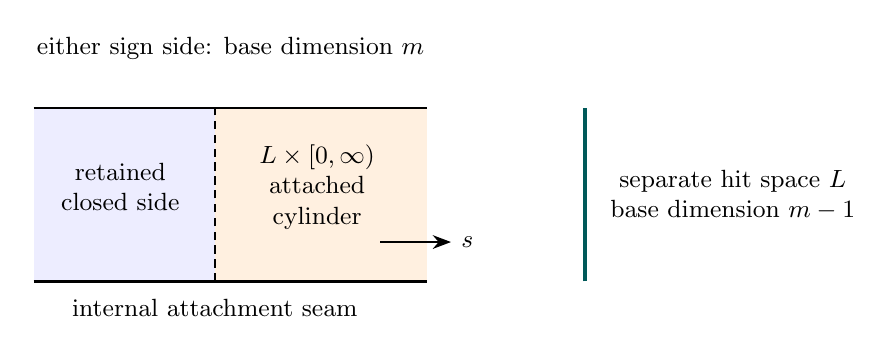
\begin{tikzpicture}[x=1cm,y=1cm,>=Stealth,font=\small]
  \fill[blue!7] (0,0) rectangle (2.3,2.2);
  \fill[orange!12] (2.3,0) rectangle (5,2.2);
  \draw[thick] (0,0) -- (5,0);
  \draw[thick] (0,2.2) -- (5,2.2);
  \draw[densely dashed,thick] (2.3,0) -- (2.3,2.2);
  \node[align=center] at (1.1,1.2) {retained\\closed side};
  \node[align=center] at (3.6,1.2) {$L\times[0,\infty)$\\attached\\cylinder};
  \draw[->,thick] (4.4,.5) -- (5.3,.5) node[right] {$s$};
  \node[align=center,below] at (2.3,-.1) {internal attachment seam};
  \draw[very thick,teal!70!black] (7,0) -- (7,2.2);
  \node[align=center,right] at (7.2,1.1) {separate hit space $L$\\base dimension $m-1$};
  \node[above] at (2.5,2.7) {either sign side: base dimension $m$};
\end{tikzpicture}
\caption{A regular cut retains each closed sign side with a full cylinder
attached, and also retains the wall as a separate hit space of one lower base
dimension. The attachment seam is internal to the extended side. In old
product ends this entire operation is a product. The raw metric and its
later smoothing are defined in Appendices~\ref{sec:cut} and~\ref{sec:regularization}.}
\label{fig:regular-packet-split}
\end{figure}


The label set and the status depth are finite in this section. The family
of connected packets may be countable; finiteness is required only for
the directed face and coface chains incident to each packet. The
downward diagram of a packet consists of that packet and all its further
faces. Numerical
requests are allocated downward through these chains before actual data
are constructed upward from faces. This does not require finite
components of the undirected incidence graph.

We now specify the analytic data that must survive each split.
For the finite-label statements in this section and the appendices we set $\sigma=1$
and use the following constants:
\begin{equation}\label{packet:constants}
\begin{gathered}
 \lambda_r=\frac14-\frac{r}{8N_*},\qquad
 b_r=1.12-\frac{.05r}{N_*},\qquad
 a_r=.60+\frac{.03r}{N_*}\quad(0\le r\le N_*),\\
 \pi_0=\frac{1}{10N_*},\qquad k=399,\qquad
 C=\frac{4k}{k+1}=3.99,\qquad
 e_0=\frac{\lambda_r-\lambda_{r+1}}{100}
     =\frac{1}{800N_*}\quad(r<N_*).
\end{gathered}
\end{equation}
Here $k$ is the number of circle factors added at each split; the initial
number may be different.  In particular $\lambda_r\ge1/8$, $a_r\le.63$,
and $1.07\le b_r\le1.12$.  The common floor $\pi_0$ and the equally
spaced stage parameters are bookkeeping for a finite list, not uniform
lower bounds for the countable construction.

\begin{definition}[Analytic invariant]\label{packet:invariant}
At stage $r$, write $J_r$ for the unprocessed labels.  On a packet $E$
of base dimension $m$, retain its base metric and all circle warps.
Write $R_E$ for the scalar curvature of that full warped metric and
$\omega_E$ for the product of its circle lengths, suppressing fixed
circle-volume constants.  Gradients of invariant functions are base
gradients; their integrals use $\omega_E\,\dd\vol_E$, and their
Laplacian is the corresponding weighted base Laplacian.
For every $j\in J_r$ the data comprise a compatible continuous profile
$\mu_j:E\to[-\infty,\infty]$ with locally Lipschitz finite truncations,
a compatible smooth potential $\Pi_j\ge\pi_0$, and compatible open
cores $U_j^+,U_j^-$ satisfying
\begin{equation}\label{packet:core-poles}
 \overline{U_j^\pm}\subset
 \operatorname{int}_E\{\mu_j=\pm\infty\}.
\end{equation}
On the open finite band the profile obeys, almost everywhere,
\begin{equation}\label{packet:profile}
 2|\grad\mu_j|\le a_r\mu_j^2+\Pi_j.
\end{equation}
Set
\begin{equation}\label{packet:required-set}
 G_j=E\setminus(U_j^+\cup U_j^-),\qquad
 D_E=\bigl\{x:\#\{j\in J_r:x\in G_j\}\ge m-1\bigr\}.
\end{equation}
The required scalar bound is
\begin{equation}\label{packet:curvature}
 R_E\ge\lambda_r+b_r\sum_{j\in J_r}\Pi_j
       \quad\hbox{on }D_E.
\end{equation}
For an unprocessed color $i$, the cores contain
$q_E^{-1}(A_i)\subset U_i^+$ and
$q_E^{-1}(B_i)\subset U_i^-$.  Enlarging cores must preserve these
conditions.  The sets $D_E$ are closed: they are finite unions of finite intersections
of the closed sets $G_j$ (and equal $E$ when the count threshold is
nonpositive).  All data are exact products
in the sense of \cref{packet:category}; at stage zero the single
space is $X$, with no product-end requirement.
\end{definition}

The threshold $m-1$ is preserved by the two kinds of output of a
split. A side keeps its dimension and loses one unprocessed label;
a hit loses both one dimension and that label. The lower threshold
$m-2$ defines a guard containing the projections of all new required
sets, even after the remaining cores have been enlarged.

\begin{lemma}[The two count inclusions]\label{packet:counts}
If $B$ is a $d$-fold further face of $E$, the product projection sends
$D_E$ in that tail into $D_B$.
At a split of label $j_0$ on a parent of dimension $m$, suppose the
remaining cores have been enlarged, giving $G'_j\subset G_j$ for
$j\ne j_0$, and define the closed guard
\begin{equation}\label{packet:guard}
 H_E^*=\bigl\{x:\#\{j\in J_r\setminus\{j_0\}:x\in G'_j\}
                      \ge m-2\bigr\}.
\end{equation}
Suppose a regular zero wall $L$ lies in $\operatorname{int}G_{j_0}$.
Pull the remaining cores to a new side or hit packet $A$ by bulk
inclusion, wall restriction, and projection of the attached cylinder.
Define $D_A$ using these cores, the remaining labels, and the dimension
of $A$, as in \eqref{packet:required-set}.
Then $D_A$ projects into both $H_E^*$ and the parent's old set $D_E$.
Guards likewise project into guards on further faces.
\end{lemma}

\begin{proof}
In an exact product tail all label memberships pull back unchanged,
whereas the face dimension is $m-d$.  A count at least $m-1$ is at
least $(m-d)-1$, proving the first assertion.  The same argument
with thresholds $m-2$ and $(m-d)-2$ proves the guard assertion.
On a new side, whose dimension is $m$, a point of $D_A$ has at least
$m-1$ remaining undecided labels.  This puts its projection in the
guard and, because $G'_j\subset G_j$, in the old required set.
On a hit packet, whose dimension is $m-1$, the required count is
$m-2$.  Its projection lies on $L\subset G_{j_0}$, so the processed
label contributes one further old undecided label.  The old count
is therefore at least $m-1$.  The cylinder projection has exactly
the same remaining memberships as its base, so the side argument
also covers all cylinder points.  These are pointwise count
statements and use no scalar estimate away from $D_E$.
\end{proof}

\begin{lemma}[Initialization and radial confinement]\label{packet:initialization}
Let the stage-zero stabilized scalar curvature be at least $.4$, and
suppose that every color pair has separation
\[
 \dist_h(A_i,B_i)>T_0+4,\qquad
 T_0=2\pi\sqrt{2/\pi_0}.
\]
Then the data of \cref{packet:invariant} exist at stage zero with
$\Pi_j=\pi_0$.  On a noncompact $X$ the radial cores can be chosen
as alternating separating subbands of a smooth proper function,
with compact smooth barrier domains around their closures lying in
the same pole plateaus.  Every regular radial partition respecting
these signs has locally finite compact wall components and compact
closed-side components before collar attachment.  On a compact $X$
a decided radial label with empty wall has the same properties.
\end{lemma}


\begin{theorem}[Finite compatible cutting]\label{finite:cut}
Fix a finite number $N_*$ of labels and the stage constants in
\eqref{packet:constants}. Suppose a stage-$r$ packet diagram is obtained by
the regular splitting construction of \cref{packet:split}, with compatible
smooth base metrics and a finite common list of positive circle warps,
and satisfies \cref{packet:invariant}. After the radial stage, require the
complete compact-part/product-end geometry of \cref{packet:category,packet:geometry}.
Let $j_0$ be the next label, and suppose every nonempty parent packet has
base dimension at least two. Then $j_0$ can be processed as follows.

On every parent there is a compatible smooth regular defining function
with the prescribed signs on the current forced core closures. Keep its
zero wall as the new hit space. To each closed sign side attach the full
product cylinder over its boundary. These pieces form a compatible smooth
stage-$(r+1)$ packet diagram with the continuous projections described
above. The wall on a parent $E$ lies in $\operatorname{int}G_{j_0}$.
The remaining profiles may first be modified, their cores enlarged,
and their potentials increased in the parents; these data are then carried to the new pieces by restriction and cylinder projection.
There are compatible smooth metrics and potentials, and exactly $399$
new positive circle factors on each new packet, for which the entire
stage-$(r+1)$ invariant holds. Earlier forced signs are preserved.
The new packets have complete compact-part/product-end geometry. This
assertion includes a possible one-dimensional output, on which its scalar
lower bound holds everywhere.

The operation fixes every old warp identically equal to $1$. For a
remaining label that is passive on the finite downward source diagrams
and the face copies used in their comparisons---constant pole profile, full corresponding core, and spatially
constant potential $c_j$ agreeing on compared faces---the construction
can preserve the pole and core and choose its new potential to be exactly
$(1+3\eta_r/2)c_j$, where $\eta_r=1/(200N_*)$.

At stage zero the single parent may instead be an arbitrary complete
smooth manifold with no product-end or bounded-geometry assumption. Subject to the same scalar and separation assumptions, if its
data are the radial initialization of \cref{packet:initialization}, the
same conclusion holds for the first split. Every resulting wall component and every closed-side component is compact before the cylinders are attached, and these components form locally finite
families.
\end{theorem}

\begin{proof}
Realize the processed profile by a smooth finite pressure and take a
local absolute minimizer of weighted perimeter minus its pressure-volume
term, as in \cref{cut:pressure,cut:bv-compactness}. The phase has the
forced signs of \cref{cut:barriers}; its boundary, called the true cut,
has the regular-part geometry of \cref{cut:gmt} but may still have
singularities. After the
radial cut, the generic pressure choice in
\cref{cut:generic-uniqueness} makes these true cuts converge to the
corresponding face products at packet ends
(\cref{cut:end-convergence}). On the initial radial parent use shift
zero and a phase from compactness; compact barriers replace this
post-radial growth and uniqueness argument.

The wall, and each retained side with its attached cylinder,
carry the quadratic-form lower bounds of \cref{cut:raw-domination}.
These bounds include a positive gradient reserve and, on a joined
side, the scalar contribution of its internal attachment seam.
They are not yet pointwise scalar bounds on smooth new packets.
Keep these true cuts and their pressures fixed. The constructions of
\Cref{local:anchors,local:sharp,shield:global} change only the remaining
profiles, enlarge their cores, and add nonnegative potentials. Their
form cost is paid by the gradient reserve and the gap
$\lambda_r-\lambda_{r+1}$, and the updated guard $H_E^*$ of
\eqref{packet:guard} misses the singular set. Thus the future required
regions can be controlled through regular portions of the true cut.
When the parent dimension is at most seven the
singular set is empty, and no singular forcing is needed; compactness on
the resulting smooth windows is the smooth case of
\cref{shield:compactness}. More generally this smooth-window case applies
whenever the limiting wall is smooth, including products of smooth faces
with Euclidean factors even when their total dimension is at least eight.
At the first radial split the same arguments
are applied on the locally finite compact transition blocks, as specified
in \cref{shield:global}.

The guarded approximation in \cref{regular:partition} now replaces
the true cut by a smooth regular wall. Its defining functions are
exact products in the old ends. The comparison with the true cut on
the guard, followed by the seam smoothing of \cref{regular:seam},
transfers the form bound to the smooth split. The positive
supersolutions of \cref{regular:correction,regular:solutions}
then supply $399$ compatible new circle factors; the scalar identity
in \cref{regular:step} converts that form bound into the pointwise
stage-$(r+1)$ scalar inequality. Throughout this transfer the parent
scalar inequality is used only over $D_E$: \cref{packet:counts}
places every new required region inside that old region as well as
inside the guard.

\Cref{packet:split,packet:geometry} give the
new geometry; \cref{packet:initialization} gives the radial confinement.
Unit entries are fixed by restriction, product extension, and seam
smoothing. For a remaining label passive in the sense stated above,
we omit its forcing updates, and
\cref{regular:constant-preservation,regular:profiles} reproduce its chosen
constant potential exactly. The choice of $\eta_r$ satisfies the strict
stage margins in \eqref{regular:eta}.
\end{proof}

This theorem is a finite-label statement. Its common positive floor and finite
list of warp factors do not provide a common floor or a global finite
list for the construction that follows. The next section proves the
stronger locality property actually needed there: on each whole packet
and each directed comparison diagram, only finitely many labels and warp
factors are nonconstant, and the remaining potential sum is a spatial
constant reproduced exactly by the construction.

\section{Countably many compatible partitions}\label{sec:countable}

The separation widths in \Cref{rounds:wide} may depend on the label.
We now use this freedom to construct the partitions. The analytic
construction is performed at finite stages. Its essential finiteness
property concerns each \emph{whole packet}, including all its infinite
product ends; local finiteness merely on compact subsets would not
suffice. The finite-label procedure is stated in \Cref{finite:cut}, and its detailed
proof is in \Cref{sec:packets,sec:cut,sec:local,sec:shield-global,sec:regularization}.
We adapt that proof using individual positive floors and finite
exceptional data on each whole packet.
This section establishes their hypotheses for the countable construction
and proves that those hypotheses persist.

\subsection{Initialization and the inductive data}

Let $D$, the centers $x_i$, and the pairs $(A_i,B_i)$ be as in
\Cref{rounds:wide}. We assume every $B_i$ is nonempty, since otherwise
$\diam_g M\le4D$. There is one label for each center, and an additional
label $0$ used first for radial confinement. The set of labels is finite
or countable; write it as $I=\{0,1,2,\ldots\}$, stopping the enumeration
if necessary. Choose
\begin{equation}\label{countable:floors}
 p_i^*>0,\qquad \sum_{i\in I}p_i^*=\frac1{20}.
\end{equation}
Use \Cref{rounds:wide} with
\begin{equation}\label{countable:widths}
 L_i=10+2\pi\sqrt{2/p_i^*}\qquad(i\ne0).
\end{equation}
We henceforth use the resulting complete metric $h\ge g$, its locally
finite list of log warps $p_\alpha$, and its stabilized scalar lower
bound $2/5$.

The initial weighted base measure is globally well defined:
\[
 \omega\,\dd\vol_h,\qquad
 \omega=\exp\Bigl(\sum_\alpha p_\alpha\Bigr)>0.
\]
The sum is locally finite. On a buffered compact set, only finitely many
nonunit factors $e^{p_\alpha}$ occur, so ordinary finite warped-product
formulas compute the stabilized scalar, weighted variations, and
invariant test forms there. These formulas agree on overlaps: adjoining
a unit factor changes none of them. In particular, the initial problem
is a weighted problem on the $n$-dimensional base $M$.

Fix numbers
\[
 0=t_0<t_1<t_2<\cdots<1,\qquad t_r\longrightarrow1,
\]
and use as many stages as there are labels. These are budget parameters,
unrelated to a spatial coordinate. Put
\begin{equation}\label{countable:constants}
 \begin{gathered}
 a_r=.60+.03t_r,\qquad b_r=1.12-.05t_r,
 \qquad \lambda_r=\frac14-\frac{t_r}{8},\\
 \Delta_r=t_{r+1}-t_r,\qquad
 e_r=\frac{\Delta_r}{800},\qquad
 \eta_r=\frac{\Delta_r}{200},\qquad k=399,
 \qquad C=\frac{4k}{k+1}=3.99.
 \end{gathered}
\end{equation}
Thus $\lambda_r\ge1/8$, $.60\le a_r<.63$, and
$1.07<b_r\le1.12$. No positive infimum of the $\Delta_r$ is required. In a stagewise
appendix lemma, its symbol $e_0$ denotes the current $e_r$.

We use the packet notation and regular splitting operation introduced in
\Cref{sec:finite-cuts}. The countable invariant below replaces the common
finite-label floor by the individual positive floors $p_j^*$.
At stage $r$, the processed labels are $0,\ldots,r-1$ and the remaining
set is $J_r$. A packet with $s$ hit entries has base dimension $m=n-s$.
Its continuous collapse map to $M$ is denoted by $q_E$. For each
$j\in J_r$ retain an extended-real continuous profile $\mu_j$ with
locally Lipschitz finite truncations, a smooth potential
$\Pi_j\ge p_j^*$, and disjoint open cores $U_j^+,U_j^-$ with
\begin{equation}\label{countable:profile-invariant}
 \overline{U_j^\pm}\subset\operatorname{int}\{\mu_j=\pm\infty\},
 \qquad 2|\grad\mu_j|\le a_r\mu_j^2+\Pi_j
 \quad\hbox{almost everywhere on the finite band}.
\end{equation}
For unprocessed center labels require
$q_E^{-1}(A_j)\subset U_j^+$ and $q_E^{-1}(B_j)\subset U_j^-$.
All data are compatible products in the packet ends. With
\begin{equation}\label{countable:required}
 G_j=E\setminus(U_j^+\cup U_j^-),\qquad
 D_E=\{x:\#\{j\in J_r:x\in G_j\}\ge m-1\},
\end{equation}
the scalar requirement is
\begin{equation}\label{countable:scalar-invariant}
 R_E\ge\lambda_r+b_r\sum_{j\in J_r}\Pi_j\quad\hbox{on }D_E.
\end{equation}
Here $R_E$ denotes the stabilized scalar expression, and integrals and
Laplacians use the product of the old warp lengths as weight. The
finiteness statement below makes these meanings unambiguous. A nonpositive
counting threshold means the whole packet.

\begin{lemma}[Initial profiles and radial blocks]\label{countable:initial}
The data in \eqref{countable:profile-invariant}--\eqref{countable:scalar-invariant}
exist at stage zero with $\Pi_i=p_i^*$. The radial forced signs can be
chosen so that every regular radial split preserving them has locally
finite compact wall and closed-side components before cylinder
attachment. On every compact radial block and buffer, only finitely
many center labels fail to be identically the negative pole with full
negative core, and only finitely many initial warps fail to be one.
\end{lemma}

\begin{proof}
For a positive number $p$, the decreasing crossing
\[
 2|y'|=.5y^2+p
\]
from $+\infty$ to $-\infty$ has length
\[
 T(p)=\int_{-\infty}^{\infty}\frac{2\,\dd y}{.5y^2+p}
      =2\pi\sqrt{2/p}.
\]
Extend it by its poles. For center $i$, begin this crossing at stretched
distance $2$ from $A_i$ and compose it with $\dist_h(A_i,\cdot)$.
The distance is $1$-Lipschitz, so the resulting profile obeys the
inequality with $.5$ in place of $a_0=.60$. Take cores
\[
 U_i^+=\{\dist_h(A_i,\cdot)<1\},\qquad
 U_i^-=\{\dist_h(A_i,\cdot)>T(p_i^*)+3\}.
\]
Their closures lie in the respective pole interiors. The stipulated
width puts $B_i$ strictly inside the negative core. In particular, on
the complement of the original closed ball $\overline B_g(x_i,2D)$,
the profile is the negative pole and the negative core is full.

There exists a smooth proper function $\rho:M\to\R$, bounded below,
with $|\rho-\dist_h(o,\cdot)|<1$ and $|\grad\rho|_h\le2$.
Here no uniform geometric assumption is necessary. To construct it,
use relatively compact coordinate balls in a locally finite cover,
convolve the distance on slightly larger balls, and blend with a
smooth partition of unity. The metric distortion and local convolution
errors can be made arbitrarily small on each ball. In differentiating
the blend, write each local approximation as the distance plus its
error; the terms involving derivatives of the partition sum to zero
on the common distance. Choose the value errors so that the remaining
partition-derivative terms have sum less than a fixed small number at
each point. A locally finite refinement and successively smaller
positive errors achieve this, while keeping the total value error
below one. Properness follows from the bounded value error and
properness of the complete metric $h$.

Choose alternating positive and negative plateaus in the $\rho$-axis,
with transition intervals wider than $2T(p_0^*)$. Rescale the preceding
crossing to these intervals, reversing its sign on alternate intervals.
The gradient bound for $\rho$ gives the profile inequality with
coefficient $.5$ and potential $p_0^*$. Choose the core closures
strictly inside the plateaus. Regular values in the remaining margins
give compact smooth barrier annuli, and a compact central barrier,
whose closures stay in the same pole plateaus. Their value bands tend
to infinity and are locally finite.

A wall respecting the signs cannot cross a separating plateau band;
each component is closed in one compact radius block and hence compact.
A component of either closed side is trapped between two separator
bands of the opposite sign, or in the initial compact block.
Regularity of the defining function gives manifold-with-boundary
charts for these sides. A compact block therefore contains only
finitely many components. The same charts prove local finiteness of
the component families. When $M$ is compact, use a radial label with
constant positive pole and full positive core; its split has no wall
and its only side is compact.

The scalar requirement initially holds everywhere because
\[
 \lambda_0+b_0\sum_i p_i^*=.25+1.12/20=.306<.4.
\]
Finally a compact block with a compact buffer meets only finitely many
original closed outer balls and finitely many initial warp supports.
Every other center label and warp has the asserted constant data there.
\end{proof}

\subsection{Finite exceptional data on entire packets}

A \emph{downward diagram} of a packet consists of it and all its further
faces. An \emph{upward diagram} consists of it and all its cofaces.
Each is finite at a fixed stage, by \Cref{packet:split}. A finite union
of either type is finite. The constructions below make finitely many
directed passes through such diagrams. They never ask for closure
under arbitrary alternating face and coface steps.

Radial confinement gives the geometric reason to expect finite data on
a whole packet. At the first split, a compact radial side or wall
component is prolonged by cylinders; its entire collapse image stays
in that original compact component. At every later split a child $A$
of $E$ has
\begin{equation}\label{countable:collapse-recursion}
 q_A=q_E\circ p_A,\qquad
 p_A=\begin{cases}
 \text{inclusion},&\text{on the wall or bulk},\\
 \text{projection to the wall},&\text{on a fresh cylinder}.
 \end{cases}
\end{equation}
Hence $q_A(A)\subset q_E(E)$, including in all simultaneous normal
directions. A finite incidence diagram therefore has image in a finite
union of compact original radial blocks. Only finitely many original
outer balls and initial nonunit warp supports meet that image.
Shielding changes no collapse map, and regularization chooses new
walls inside old parents, so both preserve this confinement.

This argument controls the initial supports. Later smooth data need
not factor through $q_A$: they also use data copied from faces. We
must therefore retain finite exceptional lists through those directed
dependencies, as well as preserve every other entry exactly.

\begin{definition}[Finite exceptional data]\label{countable:finite-data}
At stage $r\ge1$, on each whole packet $E$ there are finite sets
$I_E\subset J_r$ of label indices and $F_E$ of old warp indices such
that, for $j\notin I_E$,
\begin{equation}\label{countable:passive}
 \mu_j\equiv-\infty,\qquad U_j^-=E,\qquad U_j^+=\varnothing,
 \qquad \Pi_j\equiv c_rp_j^*.
\end{equation}
For every old warp index outside $F_E$, its length is identically one.
The number $c_r$ is the same on all packets and is prescribed by
\begin{equation}\label{countable:passive-multiplier}
 c_0=1,\qquad c_{r+1}=(1+3\eta_r/2)c_r.
\end{equation}
For any finite diagram used in a comparison, take the union of its
finite exceptional sets, adding the current label explicitly. This
one finite union then works simultaneously on all its whole packets.
At stage zero the analogous property is required on every compact
radial block and buffer, with $c_0=1$.
\end{definition}

The sets $I_E$ need not consist exactly of the nonconstant entries: an
entry may be retained in the exceptional list even if it happens to be
constant. This convention avoids any need to discard previous exceptions.
Only the existence of a finite list matters.

\begin{lemma}[Consequences and directed dependencies]\label{countable:locality}
Suppose the packet geometry and \Cref{countable:finite-data} hold at a
finite stage. Then the following assertions hold.
\begin{enumerate}[label=(\roman*),leftmargin=*]
\item The sum of potentials on a whole packet is a smooth function
with bounded derivatives of every fixed order. The undecided counts,
required sets, and guards use only a finite list and are closed.
\item On each whole packet and each finite comparison diagram, the old
weight, stabilized scalar, stability forms, and weighted Laplacian are
computed with one finite list of warps, after padding with unit factors.
The bounded geometry and polynomial weighted growth conclusions of
\Cref{packet:geometry} apply, including on any finite Euclidean product.
\item Compatible choices with positive packetwise tolerances can be
made in the following order: fix individual requests, propagate numerical
requests down the finite coface chains, and then construct data upward
from deeper faces. Enlarging a coface's exceptional list by the union
over its downward source diagram suffices for the last pass. No data
are propagated back from a newly constructed coface to an already
constructed face.
\end{enumerate}
\end{lemma}

\begin{proof}
On $E$, the sum of potentials is exactly
\begin{equation}\label{countable:potential-sum}
 \sum_{j\in J_r}\Pi_j
 =\sum_{j\in I_E}\Pi_j+c_r\sum_{j\in J_r\setminus I_E}p_j^*.
\end{equation}
The second term is a finite spatial constant. Indeed
\[
 1\le c_r\le\exp\Bigl(\frac32\sum_{s<r}\eta_s\Bigr)
 \le e^{3/400}.
\]
The first term is a finite sum; its derivative bounds follow from
compatible smoothness and the compact-part/product-end decomposition
in \Cref{packet:geometry}. On a finite comparison diagram choose common
product thresholds for its finite exceptional list. Every other entry is already a spatial
constant with the same value on each copy. The full sum is therefore
an exact face pullback beyond those thresholds; no supremum of
infinitely many thresholds is taken. Passive entries have empty
undecided set. Thus a set requiring at least $a\ge1$ undecided labels
is the finite union, over $a$-element subsets of $I_E$, of the intersections of
their closed $G_j$'s. This proves closedness, including for the guards
with threshold $m-2$. Threshold zero gives $E$.

For (ii), take the union of the finitely many relevant old warp
indices on the finite diagram and set every missing entry to one.
Writing $u_\alpha=\log f_\alpha$ and $U=\sum_\alpha u_\alpha$, the
scalar expression is
\[
 R_E=\Scal_{h_E}-2\Delta_{h_E}U-|\dd U|_{h_E}^2
                        -\sum_\alpha|\dd u_\alpha|_{h_E}^2.
\]
A padded logarithm is zero; the product weight is unchanged. The
weighted Laplacian is
$\Delta_{h_E}+\langle\dd U,\dd\,\cdot\,\rangle_{h_E}$ and is
unchanged as well. Weighted perimeter and its first and second
variations depend on the same weight. Equivalently, a flat unit
factor adds zero second fundamental form and zero curvature to the
invariant variation calculation. Thus the wall and seam forms also
agree. The finite-diagram geometric lemma now gives completeness,
bounded geometry, positive lower and finite upper bounds for the
weight, and center-uniform polynomial volume growth. It gives the
same statements after taking a finite Euclidean product. The
regularity problem for a minimizing phase remains on the base, with
singular dimension at most $m-8$ by \Cref{cut:gmt}; padding does not
alter that dimension.

For (iii), a particular face receives requests from only its finitely
many cofaces and coface chains. Allowing for the finitely many fixed
product and cutoff bounds, the minimum of the requested positive
errors is positive. Settle all these numbers before constructing the
approximations. A request only decreases an error tolerance: it does
not copy any coface value into the face. During the subsequent upward
pass, the inputs on a packet are its own data and already constructed
copies from its finite downward diagram. Their exceptional sets have
a finite union. Outside that union every copy in
\eqref{countable:passive} agrees with every other copy. A newly
constructed coface is not used to reconstruct its sources. The same
argument applies to finitely many successive directed passes, and
proves the stated dependency rule.
With these numerical tolerances fixed, at each upward pass the output
on $E$ depends only on its original data and the outputs on its strict
faces. Its source set for copied functions is therefore contained in
the finite downward diagram of $E$. The preceding downward pass changes only positive
numbers, not the input functions. In particular two packets sharing
a face do not copy one another's newly constructed data through that face.
\end{proof}

\subsection{One countable invariant step}

\begin{proposition}[Preservation of the invariant]\label{countable:step}
Suppose that all nonempty parents at stage $r$ have base dimension at
least two and satisfy \eqref{countable:profile-invariant}--\eqref{countable:scalar-invariant}.
At $r=0$ use the compact radial blocks of \Cref{countable:initial}; at
$r\ge1$ suppose also that the packet geometry and
\Cref{countable:finite-data} hold. Processing label $r$ produces the
compatible smooth split, preserves the forced signs, and gives the
same assertions at stage $r+1$. Exactly $399$ new warp factors, with
common indices, are appended at this stage. Each whole resulting
packet has a finite relevant old warp list.
\end{proposition}

\begin{proof}
We verify the choices in their order of dependence.

\emph{The current pressure and minimizing phases.}
The pressure construction of \Cref{cut:pressure} uses a positive floor
only for the label being processed. Replace its finite-family floor
by $p_r^*$. Compatible clipping heights can first be chosen above the
local barrier bounds, with a uniform extra barrier margin of one.
Then use local smoothing errors to obtain
\[
 2|\grad p_0|\le .65p_0^2+1.01\Pi_r.
\]
All smoothing requests involve only this one profile and finite
incidence diagrams. The elementary inequality
\[
 .67(y+c)^2-.65y^2\ge-21.775c^2
\]
shows that one common nonempty shift interval, for example
\begin{equation}\label{countable:shift}
 |c|<\min\{.01\sqrt{p_r^*},1/2\},
\end{equation}
preserves both $2|\grad(p_0+c)|\le .67(p_0+c)^2+1.02\Pi_r$ and
the barrier inequalities. Floors for other labels do not enter this
interval.

After the radial stage, \Cref{countable:locality} supplies all bounded
geometry and weighted polynomial-growth hypotheses of
\Cref{cut:generic-uniqueness}. There are countably many packets,
Euclidean product dimensions, and tests in that lemma's exhaustion.
Remove the countable exceptional shift sets and choose a single $c$
in \eqref{countable:shift}. The resulting true minimizers have the
common product limits of \Cref{cut:end-convergence}; choose them before
any shielding update. At the initial radial step no uniqueness or
polynomial growth at spatial infinity is used. The smooth global
positive weight and locally bounded smooth pressure give local BV
existence and strict compactness by \Cref{cut:bv-compactness}. The
relatively compact radial barriers force the phases by compact
comparisons. All variations and tests lie in buffered compact windows
with finite warp lists, so the formulas in \Cref{cut:raw-domination}
apply. The GMT and shielding dimensions are the base dimensions at
this first step as well.

\emph{Anchors, guards, and shielding.}
On each post-radial packet retain its finite exceptional list, enlarged
by its finite downward source diagram and by the current label.
Labels outside it are already forced everywhere and require no shell
addition. Choose compatible smooth clipped anchors as in
\Cref{local:anchors}, retaining the exact value $-1$ for a passive
profile. For each packet of dimension $m\ge8$ and each set of $m-7$
remaining labels, the image of its singular set under the corresponding
smooth anchor map has $(m-7)$-dimensional Lebesgue measure zero.
There are countably many such conditions, even if all finite subsets
of the countable label set are included. In the countable product of
uniform probability intervals $(-.3,.3)$, each bad cylinder has
measure zero by its finite-dimensional marginal. A threshold vector
outside their union therefore exists. At most $m-8$ anchors equal
their thresholds at any singular point. The sign exclusions at poles
follow from the $.1$ anchor approximation, exactly as in
\Cref{local:anchors}.

Process the finitely many face depths from deepest upward, keeping the
true cuts fixed. Suppose all strict faces of $E$ have been shielded.
Its remaining risky set
\[
 K_E=\Sigma_E\cap
 \{x:\#\{j\in J_r\setminus\{r\}:x\in G'_j\}\ge m-2\}
\]
is closed. It is compact: an escaping sequence would, by
\Cref{packet:escape}, have a product limit over a further face with
compact convergent base coordinates. The finite exceptional list and
closed core complements pass the undecided count to that limit.
The face has a smaller dimension, so the limit lies in its guard.
The product convergence of true cuts forces the limiting point to be
singular, since regular-point graphical convergence excludes nearby
singular points. This contradicts the completed shielding of that
face. This argument also treats escape in several normal coordinates.

Apply \Cref{local:flat-pieces,local:shell,local:sharp} on this compact
risky set, only for the finite list which can still be undecided.
Enumerate the signed compact flat pieces. Choose each shell scale by
\Cref{shield:maximum}, hold it fixed, and then send its coface fronts
far enough out by \Cref{shield:extension}. In the cap construction
of \Cref{shield:caps}, the crossing for label $j$ satisfies
\[
 2|w'|\le .58w^2+p_j^*.
\]
Its length is finite; the inequality is paid by $\Pi_j\ge p_j^*$.
The minimum-of-branches formula in that lemma adds no simultaneous
normal derivative cost. Its cutoff finishes before the cap crossing
starts, so whenever the shell branch is active the whole shell
potential is available. Opposite signs remain in disjoint strict
anchor regions, and cores only enlarge.

Only finitely many additions are required on $E$. Indeed, every point
of the initial compact $K_E$ eventually belongs to an open forced core
for each of its strict anchors among the finite exceptional list.
At most $m-8<m-2$ labels can then remain undecided there. The residual
risky subsets of the initial $K_E$ are nested and closed, and their
intersection is empty. Compactness gives a finite index at which the
residual is empty. Stop then. Each specified coface receives additions
from finitely many source faces through finitely many chains. Thus
only finitely many additions and finite minima or maxima affect any
whole packet. In particular no infinite limiting profile is taken on
that packet.

To control all the countably many packets at once, enumerate each
possible local addition and assign positive allowances with total less
than $.12$. Split each allowance between its shell-scale choice and
its simultaneous finite coface extension choices. Starting the
bookkeeping form bound at $.78$, the maximum estimate and the
extension estimate give one $\theta_*<.9$ such that
\begin{equation}\label{countable:shield-form}
 \int1.16\sum_{j\ne r}D_jv^2
 \le\theta_*\bigl(\mathcal N(v)+e_r\|v\|_2^2\bigr).
\end{equation}
Here $\mathcal N$ has coefficient $1.7$ on a wall and coefficient
$.8$ on bulk plus $1.7$ on its attached cylinder. These are the
same coefficients on every packet and product. Only a finite list of
additions occurs on each post-radial packet, so the bound persists
after a whole depth has been treated.

Initially, instead work in separated compact transition shells with
compact buffers between radial barriers. Each has finitely many
exceptional labels and warps. Its risky set is compact, and the same
finite termination applies; there is no coface extension yet. Choose
supports within the shell buffers. Their local finiteness makes all
updates locally finite on $M$, and a compact test meets only finitely
many of them. The summable allowances prove
\eqref{countable:shield-form} for every such test. Every compact radial
side block meets only finitely many shell buffers. This supplies the
whole-packet finite lists after the first attachment.

\emph{Counts and the quantitative transfer.}
Core enlargement gives $G'_j\subset G_j$. Only the finite exceptional
list can contribute to the counts on a post-radial packet; the analogous
statement holds on buffered compact blocks at the radial step.
Thus \Cref{packet:counts} places every new required set in both the old
required set and the shielded guard under projection, including along
attached cylinders. The finite lists and closed core complements also
pass these count inclusions to all further-face product limits.

The guarded tube and comparison constructions of
\Cref{regular:guards,regular:partition} use these closed guards,
regular graphical convergence on product limits, and finite
packetwise derivative bounds. All are now available. Numerical
errors are allocated down coface chains before the defining functions
are constructed upward.

Apply the quantitative transfer of \Cref{regular:transfer} with the
current $t_r$, $\Delta_r=t_{r+1}-t_r>0$, and $e_0=e_r=\Delta_r/800$.
Its stage margins \eqref{regular:eta} were proved for these general
adjacent parameters, so they do not require equally spaced stages.
The potential calculation also applies: on each finite comparison
diagram, \eqref{countable:potential-sum} expresses the old potential
sum as finitely many smooth functions plus one spatial constant.
Only finitely many shielding additions occur there. Thus, with
$\widetilde\Pi_j=\Pi_j+D_j$, the same raw form and comparison estimates
control
\begin{equation}\label{countable:raw-target}
 \lambda_{r+1}+(1+3\eta_r)b_{r+1}
                         \sum_{j\ne r}\widetilde\Pi_j
\end{equation}
near the new required set, with the positive mass and gradient reserves
proved there. The constant tail has no derivative error; potential
approximation errors concern only the finite exceptional list. At the
radial step these estimates are made on buffered compact blocks, as
in that proof.
The seam and potential smoothing can consequently retain an $e_r$
local mass gap. This positive number is fixed for the current stage;
all geometric tolerances may depend on the packet. No infimum over
future stages or over all packets is taken.

\emph{Exact passive constants in regularization.}
Restrictions, bulk inclusions, and cylinder projections preserve
identically constant functions. Seam smoothing of an old identically
unit warp leaves it one. For the remaining potentials, smooth
$(1+3\eta_r/2)\widetilde\Pi_j$ as in
\Cref{regular:profiles,regular:constant-preservation}, so that
\begin{equation}\label{countable:smooth-potentials}
 (1+\eta_r)\widetilde\Pi_j\le\Pi_j^{\rm new}
                     \le(1+2\eta_r)\widetilde\Pi_j.
\end{equation}
On a finite exceptional list, allocate the required relative errors
separately, using $p_j^*>0$ for its $j$th entry. If an aggregate error
is prescribed, subdivide it among that finite list. If an entry is
passive on the whole source diagram, set its output \emph{exactly} to
$c_{r+1}p_j^*$. This is compatible with the smoothing procedure:
local convolution of a constant is that constant, partition weights
sum to one, and every copied end value is the identical constant.
Equivalently this entry can simply be omitted from all smoothing and
restored as that constant afterward. We only impose this rule on
whole constant inputs and their agreeing copies, so it makes no claim
about preserving the edge of an arbitrary nonsmooth plateau.

Before blending on a coface, enlarge its exceptional list by the union
over its entire finite downward source diagram. Thus a face-active
entry is recorded even if the coface's individual input was passive.
The remaining copies agree identically. Coface requests merely adjust
numeric tolerances; they do not introduce new source values on faces.
This proves exact passive reproduction on the completed diagram and
precludes a cascade through infinitely many same-depth neighbors.
At the radial step choose a compact buffer for each compact radial
block, enlarged to contain the finitely many chart closures and shell
supports used by its approximations. Only finitely many original
outer balls and initial nonunit warp supports meet this buffer.
Enlarge the exceptional list by precisely these indices. Every other
entry is the same constant on every averaging neighborhood and is
therefore reproduced exactly before cylinder attachment.

The local-slope argument of \Cref{regular:profiles} justifies restriction
of profiles to the wall: an almost-everywhere gradient bound by a
continuous function gives the corresponding local Lipschitz slope
bound at every point of each finite band. Restriction and cylinder
projection then preserve it. The small metric change increases slopes
by at most $1+\eta_r$, and the first inequality in \eqref{regular:eta}
together with \eqref{countable:smooth-potentials} gives the next profile
inequality.
Continuous pullback and core enlargement preserve all pole-neighborhood
and forced-preimage conditions.

\emph{Corrections, supersolutions, and the new warp group.}
The sum in \eqref{countable:potential-sum} is now smooth, bounded, and
exactly compatible, as are its finite-order derivatives. On every
required finite diagram, pad the old warps by units. In a product end
over $B$ the operator of \Cref{regular:correction} therefore satisfies
exactly
\[
 L_A=L_B-C\Delta_{\rm normal},\qquad
 L_A=-C\Delta_{\rm old}+R_{\rm old}-V_A^*+K_A,
 \qquad
 V_A^*=\lambda_{r+1}+b_{r+1}\sum_{j\ne r}\Pi_j^{\rm new}.
\]
In particular the potential formula does not depend on the base
dimension or on how many unit factors were padded. The correction is
zero near the new required set and produces a positive form gap on
each whole packet. The proof of \Cref{regular:correction} uses finite
minima of the gaps on the packet's face diagram. Its bounded resolvent
and the compatible positive supersolutions in
\Cref{regular:resolvent,regular:solutions} apply with the packetwise
bounded geometry and polynomial weighted volume already proved.
Their tolerances are chosen after the operators and their individual
exact solutions are fixed, and before the final upward blending pass.
Thus their finite-dependency hypothesis is precisely (iii) of
\Cref{countable:locality}.

Let $v_A>0$ be the resulting supersolution with $L_Av_A\ge1/2$.
Append the common group of $k=399$ circle lengths
$f=v_A^{2/(k+1)}=v_A^{1/200}$. The scalar identity in
\Cref{regular:step} gives
\[
 R_{\rm new}=R_{\rm old}-C\frac{\Delta_{\rm old}v_A}{v_A}
           =V_A^*-K_A+\frac{L_Av_A}{v_A}
           \ge V_A^*\quad\hbox{on }D_A.
\]
Only the number of \emph{new} factors enters the coefficient $C$.
The old finite list may vary from packet to packet; unit padding has
no effect. Each stage adds just this one finite group, with the same
indices in every status. All its lengths are positive and bounded
above and away from zero on a whole packet, and exactly compatible.
The initial lists and their finite propagated exceptions remain finite,
so the complete old list at stage $r+1$ is still finite on each whole
packet and each finite comparison diagram.

Finally the regular split preserves compact truncations and finite
incidence by \Cref{packet:split}. Initially the radial separators make
all components compact before prolongation. Compatible smooth metrics
and finite relevant warps then give the complete packet geometry by
\Cref{packet:geometry}. The recursion
\eqref{countable:collapse-recursion} preserves confinement in original
radial blocks. All exceptional-list enlargements just described are
finite, and all passive constants have multiplier $c_{r+1}$.
This completes the induction step, including the first radial step.
\end{proof}

\subsection{Termination in dimension and finite-stage walls}

\begin{lemma}[The one-dimensional obstruction]\label{countable:dimension-one}
No nonempty one-dimensional packet can satisfy the invariant at a
finite stage of the construction.
\end{lemma}

\begin{proof}
Such a packet is complete by \Cref{packet:geometry} and has only
finitely many relevant positive smooth warps $f_1,\ldots,f_q$ on
its whole base. Its arclength universal cover is $\R$, including
when the packet itself is a circle. On this line put
$u_\alpha=\log f_\alpha$ and $P=\sum_{\alpha=1}^q u_\alpha$.
The warped-product scalar formula reduces to
\[
 R=-2P''-(P')^2-\sum_{\alpha=1}^q(u_\alpha')^2.
\]
The required count in dimension one is zero, so the invariant holds
everywhere and gives $R\ge\lambda_r>0$. Consequently
\[
 -2P''\ge\lambda_r+(P')^2,\qquad
 \frac{\dd}{\dd s}\arctan\frac{P'}{\sqrt{\lambda_r}}
 \le-\frac{\sqrt{\lambda_r}}2.
\]
Integration over a line interval longer than
$2\pi/\sqrt{\lambda_r}$ contradicts the range of the arctangent.
If $q=0$, the scalar formula is simply $R=0$. The argument takes
place at one finite stage and uses an ordinary finite sum.
\end{proof}

\begin{proposition}[The countable compatible construction]\label{countable:construction}
All labels can be processed successively. At every finite stage the
packet diagram has the invariant above and no nonempty packet of
dimension at most one. After the radial stage it has finite exceptional
data on whole packets; at stage zero this assertion holds on buffered
compact radial blocks.
Its finite reconstruction $X_r$ has a proper collapse $q_r:X_r\to M$
and closed signed sides $P_i^{(r)},N_i^{(r)}$ for each processed center
label, with
\[
 P_i^{(r)}\cup N_i^{(r)}=X_r,\qquad
 P_i^{(r)}\cap N_i^{(r)}=W_i^{(r)},
\]
where $W_i^{(r)}$ is its wall. The forced preimages satisfy
\[
 q_r^{-1}(A_i)\subset P_i^{(r)}\setminus W_i^{(r)},\qquad
 q_r^{-1}(B_i)\subset N_i^{(r)}\setminus W_i^{(r)}.
\]
These inclusions hold in open phases and persist at every subsequent
finite stage. No $n-1$ distinct walls, even including the radial wall,
have a common point. Each center wall lies over its original open
outer ball, and its components are compact and locally finite.

Old horizons can be enlarged by identifications preserving collapse,
all walls, and all signed statuses. For any prescribed sequence
$\eps_r>0$ with $\sum_r\eps_r<1$, the next finite collar compression
can be chosen with collapse displacement less than $\eps_r$, preserving
the previously decided wall strata and signed sides. These are
finite-stage conclusions; the limiting fixed-copy construction is
made in the next section.
\end{proposition}

\begin{proof}
Initialization is \Cref{countable:initial}. If the construction has
reached stage $r$, its parents have dimension at least two: a first
nonempty output of smaller dimension would have dimension exactly
one, since a hit decreases dimension by one and a sign preserves it.
\Cref{countable:step} produces the next invariant, and
\Cref{countable:dimension-one} excludes that first output. Thus the
induction continues through every finite stage. There is no passage
to an infinite-stage analytic metric, weight, or torus.

Apply \Cref{packet:reconstruction} to each finite initial segment.
Its hypotheses are the regular compatible splits and the compact
radial components already established. Its status pieces are exactly
the corresponding compact packet truncations. If $n-1$ walls met,
assign those labels hit status and choose a closed sign status for
each other processed label containing the point. The corresponding
nonempty truncation would have dimension one, a contradiction.
Forced signs persist under the continuous collapse recursion and
enlargement of the cores. In particular
\[
 q_r(W_i^{(r)})\subset M\setminus(A_i\cup B_i)
                         \subset B_g(x_i,2D).
\]
Properness of $q_r$ and compactness of the original closed outer ball
make each wall component compact; regular local wall charts give
local finiteness, as in \Cref{packet:reconstruction}.

The horizon identifications in \Cref{packet:reconstruction} preserve
collapse, walls, and signed statuses. Its collar compressions preserve
the old strata and their sides, and \Cref{packet:small-displacement}
allows their collapse oscillations to be bounded by the prescribed
$\eps_r$. These choices are made separately on the locally finite
compact component family; no uniform collar width or horizon at
infinity is required. The next section chooses these finite-stage
homeomorphisms coherently on one fixed copy of $M$.
\end{proof}

\section{Reconstruction and the map to a complex}\label{sec:reconstruction}

All distances in this section are measured in the original metric $g$;
write $d_0$ for that distance.  Put $D=WR_0$, as in
\cref{rounds:wide}.  The centers $x_i$ form a maximal $D$-separated set,
and the color pairs are
\[
 A_i=\overline B_0(x_i,D),\qquad
 B_i=M\setminus B_0(x_i,2D).
\]
The $A_i$ cover $M$.  Every family of balls with these centers and a
fixed finite radius is locally finite: a compact set has a compact
neighborhood of that radius by completeness, and a compact metric
space contains only finitely many $D$-separated points.  The family is
countable, since $M$ is second countable.  If some $B_i$ is empty,
$\diam_{g}M\le 4D$ and a constant map proves the theorem.  We therefore
assume that all $B_i$ are nonempty.

\subsection{A limit on the original manifold}

The analytic packets have infinite product ends.  Their finite
reconstructions in \cref{packet:reconstruction} are manifolds
homeomorphic to $M$; only finite intervals of the product ends are used
in these reconstructions.  We now choose those homeomorphisms
coherently.  This is the point at which local finiteness of the color
supports is essential.

\begin{proposition}[Reconstructed partitions]\label{topology:partitions}
The compatible cuts of \cref{countable:construction} give a continuous
proper map $q:M\to M$, and for every color $i$ closed sets $P_i,N_i,W_i$
such that
\begin{align}
 &d_0(q(x),x)<1,\label{topology:displacement}\\
 &P_i\cup N_i=M,\qquad P_i\cap N_i=W_i,
   \qquad W_i\subset q^{-1}\bigl(B_0(x_i,2D)\bigr),
   \label{topology:sides}\\
 &q^{-1}(A_i)\subset P_i\setminus W_i,
   \qquad q^{-1}(B_i)\subset N_i\setminus W_i.
   \label{topology:forced}
\end{align}
The wall family $(W_i)$ is locally finite, and no $n-1$ distinct walls
have a common point.
\end{proposition}

\begin{proof}
Choose positive numbers $\eps_0,\eps_1,\ldots$ with
$\sum_{r\ge0}\eps_r<1$.  Here $\eps_0$ is assigned to the single radial
stage; the other numbers are assigned to successive color stages.
In this proof only, index the post-radial reconstruction by $r=0$.
For a finite reconstruction write
\[
 q_r:X_r\longrightarrow M,\qquad
 H_r:X_r\longrightarrow M,\qquad
 Q_r=q_r\circ H_r^{-1}.
\]
The map $q_r$ is the proper collapse of
\cref{packet:reconstruction}, whereas $H_r$ is a homeomorphism to a
fixed copy of the original manifold.  We maintain
\begin{equation}\label{topology:finite-error}
 d_0(Q_r(x),x)\le E_r,
 \qquad E_r\le\sum_{j=0}^{r}\eps_j<1.
\end{equation}
Walls and their two closed sides will also be viewed on this fixed copy
using $H_r$.

For the radial stage, the cut has a locally finite family of compact
components.  Choose pairwise disjoint, locally finite collars of these
components on which the collapse varies by less than $\eps_0$ in each
normal segment.  Compactness of each component and continuity of the
collapse permit the collars to be this small, independently from one
component to another.  Compress the finite inserted cylinders into
these collars.  Since their supports are disjoint, the displacement
bound is $\eps_0$, rather than a sum over components.  This constructs
$H_0$ and proves \eqref{topology:finite-error} initially.  The finite
length of an inserted cylinder may be arbitrarily large; its length
does not impose a lower bound on the width of the collar into which it
is compressed.

We describe a subsequent color stage $i$.  First raise any old finite
horizons needed for the new compatible defining functions.  Denote the
resulting reconstruction by $\widehat X_r$.  The horizon
reparameterization
\[
 \Phi_r:\widehat X_r\longrightarrow X_r
\]
preserves collapse and every old wall and signed side.  Indeed, on an
old product end the collapse is independent of the normal coordinate,
and an increasing change of that coordinate preserves its sign and its
zero section.  Compatible products of these changes agree at corners.
Thus we may set
\begin{equation}\label{topology:horizon}
 \widehat q_r=q_r\circ \Phi_r,\qquad
 \widehat H_r=H_r\circ \Phi_r,
 \qquad
 \widehat q_r\circ\widehat H_r^{-1}=Q_r.
\end{equation}
In particular, increasing a horizon contributes no displacement on the
fixed copy.

The new wall lies over $B_0(x_i,2D)$.  Choose its collar strip $S_i$ in
$\widehat X_r$ so that
\begin{equation}\label{topology:strip}
 S_i\subset\widehat q_r^{-1}\bigl(B_0(x_i,2D+1)\bigr),
\end{equation}
and so that collapse oscillation along every segment used by the
compression is less than the error assigned to this stage.  These
choices are possible because the relevant wall components in a finite
reconstruction are compact and locally finite.  More specifically,
their union lies in the inverse image of the compact ball
$\overline B_0(x_i,2D)$ under the proper finite collapse; hence only
finitely many components are involved in this color stage.

The strips can be chosen to preserve every old stratum, including the
radial strata.  To check this assertion, work near a point of a new wall
on an old stratum, and denote the new defining function by $u$.
The horizons were chosen beyond the product thresholds, so the terminal
collars glued at each old hit wall lie in the product range.  In the
resulting product chart, $u$ is pulled back from the corresponding face
and is independent of the old signed normal coordinates.  Its restriction
to that face is regular at zero.  In the corresponding product chart choose a vector field
$V$ in the face directions with $V(u)=1$, and with zero component in
every old normal direction.  The chart may avoid the old walls not
passing through the point.  A partition of unity combines these fields:
the linear identity $V(u)=1$ and tangency to every old wall both survive.
Its short flow supplies a collar preserving the old walls and their
sides.  On a fresh cylinder, each old stratum is the product of its
intersection with the new wall and the cylinder interval.  The
compression uses the same increasing normal reparameterization on
all these products.  It consequently preserves every old signed side
as well as all their intersections.

Let
\[
 c_r:X_{r+1}\longrightarrow\widehat X_r
 \quad\hbox{and}\quad
 h_r:X_{r+1}\longrightarrow\widehat X_r
\]
be, respectively, the new cylinder collapse and the homeomorphism that
compresses those cylinders into the chosen strips.  They agree off
the inverse image of $S_i$. Figure~\ref{fig:topology-compression} shows
the two maps schematically in a normal coordinate: $c_r$ collapses the
inserted interval, while $h_r$ compresses it into the chosen old collar.
Define
\begin{equation}\label{topology:recursion}
 q_{r+1}=\widehat q_r\circ c_r,
 \qquad H_{r+1}=\widehat H_r\circ h_r,
 \qquad
 Q_{r+1}=\widehat q_r\circ c_r\circ h_r^{-1}
                         \circ\widehat H_r^{-1}.
\end{equation}
The oscillation choice gives
$d_0(Q_{r+1}(x),Q_r(x))<\eps_{r+1}$ wherever they differ, proving
\eqref{topology:finite-error} at the next stage.  Their difference is
supported in $\widehat H_r(S_i)$.  If
$x=\widehat H_r(z)$ belongs to this set, then
\eqref{topology:horizon}, \eqref{topology:strip}, and
\eqref{topology:finite-error} imply
\begin{equation}\label{topology:fixed-support}
 d_0(x,x_i)
 \le d_0(x,Q_r(x))+d_0(\widehat q_r(z),x_i)
 <1+(2D+1)=2D+2.
\end{equation}
This support radius is independent of the stage.

\begin{figure}[!b]
\centering
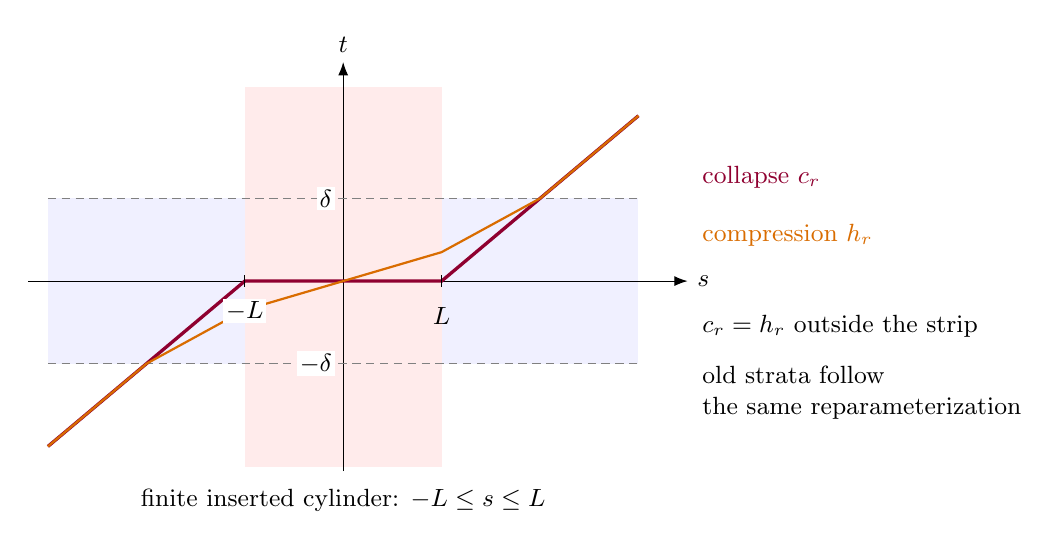
\begin{tikzpicture}[x=1.25cm,y=1.05cm,>=Latex,font=\small]
 \fill[blue!6] (-3,-1) rectangle (3,1);
 \fill[red!8] (-1,-2.25) rectangle (1,2.35);
 \draw[->] (-3.2,0)--(3.5,0) node[right] {$s$};
 \draw[->] (0,-2.3)--(0,2.65) node[above] {$t$};
 \draw[densely dashed,gray] (-3,1)--(3,1);
 \draw[densely dashed,gray] (-3,-1)--(3,-1);
 \draw[very thick,purple!75!black]
  (-3,-2)--(-1,0)--(1,0)--(3,2);
 \draw[thick,orange!85!black]
  (-3,-2)--(-2,-1)--(-1,-.35)--(0,0)--(1,.35)--(2,1)--(3,2);
 \draw (-1,.07)--(-1,-.07) node[below=4pt,fill=white,inner sep=1pt] {$-L$};
 \draw (1,.07)--(1,-.07) node[below=4pt] {$L$};
 \node[left,fill=white,inner sep=1pt] at (-.08,1) {$\delta$};
 \node[left,fill=white,inner sep=1pt] at (-.08,-1) {$-\delta$};
 \node[align=left,anchor=west,text=purple!75!black] at (3.55,1.25)
  {collapse $c_r$};
 \node[align=left,anchor=west,text=orange!85!black] at (3.55,.55)
  {compression $h_r$};
 \node[align=left,anchor=west] at (3.55,-.55)
  {$c_r=h_r$ outside the strip};
 \node[align=left,anchor=west] at (3.55,-1.35)
  {old strata follow\\the same reparameterization};
 \node[below,align=center] at (0,-2.4)
  {finite inserted cylinder: $-L\le s\le L$};
\end{tikzpicture}
\caption{The two maps used in a finite reconstruction, shown schematically
in local normal coordinates: $s$ on the reconstructed domain $X_{r+1}$
and $t$ on the old target $\widehat X_r$. The target strip $|t|<\delta$
represents the chosen collar $S_i$.
The collapse is constant on the inserted cylinder;
the homeomorphism squeezes it into an arbitrarily narrow old collar.
Where the maps differ, both images lie in the target strip.  Infinite analytic ends
are truncated before this topological operation.}
\label{fig:topology-compression}
\label{packet:collar-figure}
\end{figure}

The balls in \eqref{topology:fixed-support} form a locally finite
family.  Consequently, on every relatively compact neighborhood in
the fixed copy, the maps $Q_r$ are exactly unchanged after finitely
many stages.  Their locally stationary limit $q$ is continuous and
satisfies \eqref{topology:displacement}.  It is proper: the inverse
image of a compact set is a closed subset of its compact closed
$1$-neighborhood in $(M,d_0)$.

At each finite stage the signed sides are the closed reconstructed
sides, with their intersection equal to the central wall.  The
stratum-preserving identifications just constructed preserve every
previously installed side and wall exactly.  Newly installed color
walls are confined to the fixed balls in
\eqref{topology:fixed-support}.  Thus all the partition data are locally
eventually unchanged.  Their final closed sets satisfy
\eqref{topology:sides} and \eqref{topology:forced}, since these are the
finite-stage forced-sign properties of
\cref{countable:construction}, and both collapse and statuses are
stationary near each point.  The wall family is locally finite by the
same support bound.  Finally, a point on $n-1$ distinct final color
walls would, on a neighborhood where these data have stabilized, lie
on the same $n-1$ finite-stage walls.  This contradicts
\cref{countable:construction}.
\end{proof}

\subsection{Thickening the walls without increasing their multiplicity}

Put $k=n-2$.  We need open neighborhoods of the whole walls, rather
than independently chosen neighborhoods of their individual compact
pieces.

\begin{lemma}[Simultaneous wall neighborhoods]\label{topology:thicken}
There are locally finite open sets $T_i\supset W_i$ such that
\begin{equation}\label{topology:thickening}
 T_i\subset q^{-1}\bigl(B_0(x_i,2D)\bigr)
                  \setminus q^{-1}(A_i\cup B_i),
 \qquad
 \#\{i:x\in T_i\}\le k\quad(x\in M).
\end{equation}
\end{lemma}

\begin{proof}
Set $O_i=q^{-1}(B_0(x_i,2D))$ and
$F_i=q^{-1}(A_i\cup B_i)$.  By
\cref{topology:partitions}, $W_i$ is disjoint from the closed set $F_i$
and lies in the open set $O_i$.  At a point $x$, local finiteness and
closedness of the walls give an open neighborhood meeting only walls
that contain $x$.  Shrink it to a neighborhood $U_x$ contained in
$O_i\setminus F_i$ for every such wall.  Therefore $U_x$ meets at most
$k$ walls, and
\begin{equation}\label{topology:cover-property}
 U_x\cap W_i\ne\varnothing\quad\Longrightarrow\quad
 U_x\subset O_i\setminus F_i.
\end{equation}

Choose a locally finite open star refinement $\mathcal V$ of this
cover: the union of the members of $\mathcal V$ meeting any fixed
member is contained in some $U_x$.  For completeness, such a refinement
can be obtained directly with the metric $d_0$.  The function
\[
 \rho(x)=\sup_U\min\{1,d_0(x,M\setminus U)\},
 \qquad U\in\{U_x:x\in M\},
\]
is positive and $1$-Lipschitz, with distance to the empty set truncated
to $1$.  The balls $V_x=B_0(x,\rho(x)/8)$ star-refine the original
cover.  Indeed, if $V_y$ meets $V_x$, the Lipschitz inequality gives
$d_0(x,y)<2\rho(x)/7$, and hence
$V_y\subset B_0(x,25\rho(x)/56)$.  The latter ball is contained in
$B_0(x,\rho(x)/2)$, which lies in a member of the original cover.
Fix $o\in M$.  Obtain a locally finite open refinement of $(V_x)$ by covering each
compact annulus
$\overline B_0(o,m)\setminus B_0(o,m-1)$ with finitely many open subsets
of members of $(V_x)$ lying in
$\{m-2<d_0(o,\cdot)<m+1\}$, for $m\ge1$.
These sets cover $M$ and are locally finite.  A refinement of a star
refinement is still a star refinement of the original cover, which
proves the assertion about $\mathcal V$.

Define
\[
 T_i=\bigcup\{V\in\mathcal V:V\cap W_i\ne\varnothing\}.
\]
It contains $W_i$, and \eqref{topology:cover-property} implies the
containment in \eqref{topology:thickening}.  If $z$ belongs to several
$T_i$, choose $V_0\in\mathcal V$ containing $z$.  For each such $i$
there is a $V_i\in\mathcal V$ containing $z$ and meeting $W_i$.
All the $V_i$ meet $V_0$, so their union lies in a single $U_x$.
That $U_x$ meets each of these walls, and therefore there are at most
$k$ of them.  Finally, $(T_i)$ is locally finite because $T_i\subset O_i$
and the family $(O_i)$ is locally finite.
\end{proof}

\subsection{Coordinates, triangulation, and entire fibers}

For each $i$ the closed sets
\[
 C_i^+=P_i\setminus T_i,\qquad C_i^-=N_i\setminus T_i
\]
are disjoint and cover $M\setminus T_i$.  For a closed set $C$ write
$\delta_C(x)=\min\{1,d_0(x,C)\}$, with $\delta_\varnothing=1$, and put
\begin{equation}\label{topology:coordinates}
 t_i(x)=\frac{\delta_{C_i^-}(x)}
                    {\delta_{C_i^-}(x)+\delta_{C_i^+}(x)}.
\end{equation}
The denominator is positive because the two closed sets are disjoint.
These continuous coordinates have the following properties:
\begin{enumerate}[label=(\roman*)]
 \item $t_i=1$ on $q^{-1}(A_i)$ and $t_i=0$ on $q^{-1}(B_i)$;
 \item $0<t_i(x)<1$ implies $x\in T_i$;
 \item $\supp t_i\subset q^{-1}(\overline B_0(x_i,2D))$,
       so the coordinate supports are locally finite;
 \item at every point at least one coordinate equals $1$, and at most
       $k$ coordinates lie strictly between $0$ and $1$.
\end{enumerate}
Here the last assertion uses the inner-ball cover and
\cref{topology:thicken}.

Consider the cubical set of finitely supported coordinate vectors
described by these properties.  Its cubes are
\[
 Q(S,A)=\{t:t_i=1\ (i\in S),\ 0\le t_i\le1\ (i\in A),
                    \ t_i=0\ (i\notin S\cup A)\},
\]
where $S,A$ are disjoint finite sets of labels, $S\ne\varnothing$, and
$|A|\le k$.  Triangulate each cube by the staircase triangulation: for
every ordering $a_1,\ldots,a_j$ of $A$, take the simplex with vertices
\begin{equation}\label{topology:staircase}
 \mathbf1_S,\quad \mathbf1_{S\cup\{a_1\}},\quad\ldots,\quad
 \mathbf1_{S\cup A}.
\end{equation}
The triangulations agree on faces: setting a free coordinate to zero
removes it, while setting it to one moves it to $S$.  They therefore
define a simplicial complex $K$ of dimension at most $k$.

We use the usual polyhedral topology on $|K|$.  To verify continuity
without placing a product topology on the infinite coordinate space,
fix a point of $M$ and a neighborhood meeting only finitely many
coordinate supports.  On that neighborhood all other coordinates
are identically zero.  The vector $(t_i)$ thus takes values in the
finite cubical complex using this finite set of labels, and is a
continuous map to that complex.  Its staircase triangulation is a
finite geometric simplicial complex, whose inclusion in $|K|$ is
continuous.  The coordinate map consequently defines a continuous map
\begin{equation}\label{topology:final-map}
 F:M\longrightarrow |K|,\qquad \dim K\le n-2.
\end{equation}
The triangulation retains the entire coordinate vector: the affine
map from each simplex in \eqref{topology:staircase} to its coordinate
simplex agrees on faces and is injective on their union.  One can see
injectivity by restricting any two finite supports to their finite
union; there it is the usual triangulation of a cubical complex.
Thus $F(x)=F(y)$ implies $t_i(x)=t_i(y)$ for every $i$.

Choose, for any two points of the same fiber, a coordinate that equals
$1$ at the first point.  It also equals $1$ at the second.  By (i), both
collapse images lie in the same open outer ball, and hence
\[
 d_0(x,y)
 \le d_0(x,q(x))+d_0(q(x),x_i)
       +d_0(x_i,q(y))+d_0(q(y),y)
 <4D+2.
\]
This applies to every pair of points in the fiber, regardless of its
number of components.  Consequently
\begin{equation}\label{topology:fiber-bound}
 \sup_{z\in|K|}\diam_{g}F^{-1}(z)\le4D+2=4WR_0+2.
\end{equation}
Together with \cref{rounds:wide,countable:construction}, this proves
\cref{thm:main}.

\section{Universal covers and the uniform simplex metric}
\label{sec:closed-covers}

We use the continuous macroscopic dimension of a metric space $X$:
$\dim_{\mathrm{mc}}X\le d$ means that a continuous map from $X$ to a
simplicial complex of dimension at most $d$, with its uniform simplex
metric, has uniformly bounded entire fibers.  Here each simplex is a
standard Euclidean simplex with the same edge length.  This is the
continuous convention in \citet[Definitions~1.1--1.2]{dranishnikov2014}.
We first convert the map already constructed to this target metric.
We then supply the two lower dimensions using the classical geodesic
index argument and the width theorem of Liokumovich and Wang.

\begin{lemma}[Changing the simplex metric without changing fibers]
\label{cover:uniform}
Let $k\ge0$ be an integer.  Suppose continuous functions $t_i:Y\to[0,1]$ have locally finite
supports, at least one equals $1$ at each point, and at most $k$ are
strictly between $0$ and $1$.  Their coordinate map admits an injective
conversion to a simplicial complex of dimension at most $k$ with its
uniform simplex metric.  The converted map is continuous, and two of
its values agree if and only if all the original coordinates agree.
\end{lemma}
\begin{proof}
Use the cubes $Q(S,A)$ and staircase simplices of
\eqref{topology:staircase}, where $S,A$ are disjoint finite sets,
$S\ne\varnothing$, and $|A|\le k$.  Realize the abstract simplices
as standard simplices, and send each coordinate simplex to its new
realization with the same barycentric coordinates.  The rules agree
on common faces.  Equality of two images identifies their minimal
simplex and its positive barycentric coordinates; the affine
combination of the corresponding finite indicator vectors recovers
the same original coordinate vector.  Thus the conversion is injective.

For $k\ge1$, give each simplex edge length $1$ and define $d_K$
as the infimum of the total Euclidean lengths of finite piecewise
straight paths in the simplices.  This infimum is finite: vertices
$\mathbf1_S$ and $\mathbf1_T$ are joined by adding the coordinates
in $T\setminus S$ and then removing those in $S\setminus T$, always
retaining a nonempty set of coordinates equal to $1$.  Every point
is joined to a vertex in its simplex.  For a vertex $v$, its
barycentric coordinate $b_v$, set to zero on simplices not containing
$v$, agrees on faces and is $\sqrt2$-Lipschitz on each unit-edge
simplex.  Indeed such a simplex is realized by the vectors
$e_v/\sqrt2$ in a Euclidean coordinate space.  Hence
\[
 |b_v(x)-b_v(y)|\le\sqrt2\,d_K(x,y).
\]
The barycentric coordinates distinguish points, so $d_K$ is a genuine
finite metric.  For $k=0$ use the discrete vertex metric.

Near a point of $Y$, only a finite set $F$ of coordinates can be
nonzero.  The coordinate map there lands continuously in the finite
cubical subcomplex with all other coordinates zero.  The conversion
is continuous on each of its closed simplices and hence on the finite
complex.  Inclusion into the full uniform realization is continuous
on a simplex because distance there is at most the length of its
straight segment.  Finite pasting therefore proves continuity on
the entire finite subcomplex, and thus near every point of $Y$.
The same local finite argument applies for $k=0$.  No equality between two topologies on an arbitrary
infinite complex is required.
\end{proof}

\begin{lemma}[Level components of a proper Morse function]
\label{cover:reeb}
Let $u:N\to\R$ be a proper Morse function on a connected smooth
manifold without boundary.  There is a locally finite simplicial graph $K$ and a
continuous map $q:N\to K$, with $K$ carrying its uniform simplex
metric, whose point fibers are precisely the connected components
of the levels of $u$.
\end{lemma}
\begin{proof}
Choose an auxiliary smooth Riemannian metric on $N$ to define gradients.
The critical set is closed and its points are isolated.  Properness
therefore makes the number of critical points in any compact slab
$u^{-1}([a,b])$ finite.  Thus the critical values form a locally finite
subset of $\R$, even if several critical points have the same value.
Every level is compact and locally path connected: regular charts
give a hypersurface, while the Morse normal form at a critical point
gives the zero set of a nondegenerate quadratic form, which is a cone
or an isolated point.  A compact locally path connected space has finitely
many components, since its components are open and form an open cover.

Let $S$ consist of the critical values and the integers.  It is
locally finite.  At each $a\in S$ put a vertex for every component
of $u^{-1}(a)$.  Between consecutive values $a<b$ of $S$, the flow of
$\nabla u/|\nabla u|^2$ identifies $u^{-1}((a,b))$ with a regular
level times $(a,b)$.  The flow exists for each compact subinterval
because its trajectory stays in a compact slab.  Each of the finitely
many connected product components defines an open edge, parametrized
by its $u$-value.  The image of a proper map to $\R$ is closed;
any finite endpoint of $u(N)$ is an attained extremum and hence a
critical value.  Thus no further finite endpoints are missing.

An edge component $E$ has a unique attachment at each end.  At its
lower end, the nonempty compact connected sets
\[
 \overline{E\cap u^{-1}((a,a+\epsilon])},
 \qquad 0<\epsilon<b-a,
\]
are nested as $\epsilon\downarrow0$.  Their intersection equals
$\overline E\cap u^{-1}(a)$: a point of this latter set is approached
by points of $E$ whose heights tend to $a$, and therefore belongs
to every displayed closure.  The intersection is nonempty,
connected and contained in $u^{-1}(a)$, hence in exactly one of that
level's components.  Attach the edge to its vertex.  The same argument
applies at $b$.  There are finitely many edges in either adjacent slab,
so every vertex has finite valence.  The resulting graph is countable
and locally finite.  Its points correspond exactly to the connected
components of all levels, using full level components as vertices
when critical values coincide.

Define $q$ by this correspondence.  On an open edge it is continuous
by the product description.  At a vertex corresponding to a compact
level component $C\subset u^{-1}(a)$, an adjacent edge not attached
to $C$ has no sequence approaching $C$: such a sequence would put
a point of $C$ into its endpoint intersection, contrary to its unique
attachment.  The finitely many other components of $u^{-1}(a)$ are
disjoint compact sets.  A neighborhood of $C$ can therefore exclude
them and the finitely many nonincident edges.  Requiring also that
$|u-a|$ be sufficiently small places its remaining points in any
prescribed short tails of the finitely many incident edges.  This
proves continuity at the vertex and shows that its whole inverse
image is $C$. The graph is connected, since $q$ is a continuous
surjection and $N$ is connected.

Subdivide every edge once with a different midpoint vertex for each
edge.  This removes parallel edges from the abstract realization;
loops do not occur because the endpoint heights differ.  The result
is a simplicial graph.  Give each new edge the same length.  Finite
valence implies that its ordinary graph topology equals the topology
of this uniform simplex metric: vertex neighborhoods contain short
segments on each of finitely many incident edges.  The subdivision
and change of edge lengths preserve points and fibers.  Thus $q$
has the asserted continuity and exact fibers.
\end{proof}

\begin{proof}[Proof of \cref{cover:main}]
Put $s=\min_M\Scal_h>0$ and $X=\widetilde M$.  The lifted metric
is complete.  If $X$ is compact, use a constant map to a vertex,
whose only nonempty fiber has finite diameter.

For $n\ge4$, the complete metric $s\widetilde h$ has scalar
curvature at least $1$.  Apply \Cref{thm:main} using the coordinates
of \eqref{topology:coordinates}, then \Cref{cover:uniform}.  Local
finiteness of their supports was proved in
\Cref{sec:reconstruction}, and the conversion preserves their
entire fibers.  Scaling back gives the bound $C_n/\sqrt{s}$ in
the original metric.

For $n=2$, the Gaussian curvature of the cover is at least $s/2$.
If a unit-speed minimizing geodesic had length $L>\pi\sqrt{2/s}$,
take a parallel unit normal $E$ along it and the endpoint-zero
variation field $V(t)=\sin(\pi t/L)E(t)$.  Its index form obeys
\[
 I(V,V)=\int_0^L\bigl(|\nabla_tV|^2-K|V|^2\bigr)\,dt
 \le \frac{\pi^2}{2L}-\frac{sL}{4}<0,
\]
contradicting minimality.  Completeness supplies minimizing geodesics,
so the cover has diameter at most $\pi\sqrt{2/s}$ and is compact
by Hopf--Rinow.  The constant map therefore proves this case.

Finally let $n=3$ and $X$ be noncompact.  Apply
\citet[Theorem~1.1, arXiv version~1]{liokumovichWang2023} to the
complete metric $(s/6)\widetilde h$, whose scalar curvature is at
least $6$.  It gives a proper Morse function such that every
connected component of every level, including critical levels, has
ambient diameter less than $18\pi$ in that metric.  Apply
\Cref{cover:reeb}.  Each whole fiber of its graph map is one such
level component, so in the original lifted metric it has diameter
less than $18\pi\sqrt{6/s}$.  This is a continuous map to a
one-dimensional uniform simplicial complex, as required.
\end{proof}

The low-dimensional conclusions use their stated classical and public
inputs.  The quantitative theorem in dimensions at least four has
the separate proof given above.  All map statements here are continuous;
changing the simplex metric does not supply a Lipschitz bound.

\appendix
\section{Packets, finite horizons, and the induction invariant}\label[appendix]{sec:packets}

This appendix gives the geometry and bookkeeping for a finite number of
partitions.  The minimization, shielding, and regularization arguments
in the following appendices construct the regular cuts to which this
geometry applies.  The passage to countably many labels is proved in
\cref{countable:construction}.

The packet diagrams, finite stage constants, analytic invariant, and
radial initialization are stated in \Cref{sec:finite-cuts}. We prove here
their geometric properties and the compatibility of finite reconstructions.

\subsection{Product ends and regular splitting}

\begin{lemma}[Compatible splitting and finite truncations]\label{packet:split}
Suppose a packet diagram after the radial stage has the properties in
\cref{packet:category}.  On every packet let $g_E$ be a smooth compatible
function, with $0$ a regular value, including on every face.
Keep $L_E=g_E^{-1}(0)$ as the new hit space.  To each closed side
$\{\pm g_E\ge0\}$ attach $L_E\times[0,\infty)$ along its boundary.
Use smooth normal collars across the attachment, chosen as products
in all sufficiently far old tails.  Connected components of these
spaces, with the appended statuses, form a new packet diagram.

It has finite face and coface incidence, properly embedded closed tails,
and compact remainders.  Each packet admits a compact truncation which
is a smooth manifold with corners and is a strong deformation retract
of the full packet.  Truncations can be chosen simultaneously on every
finite downward diagram, with their faces equal to the corresponding
truncated packets.  If thresholds are in the product range of $g_E$,
the old retractions preserve its zero set and both closed sides.
These conclusions also hold at the first radial stage provided that,
before attachment, its wall and closed-side components are compact and
form a locally finite family in $X$.
\end{lemma}

\begin{proof}
First work in the finite downward diagram of one old packet.  Raise
all entry thresholds until every overlap is in a commuting quadrant,
and until all the functions in this diagram are products there.
For an elementary normal coordinate $t_i$ choose a larger horizon $h_i$.
On its tail use
$t_i\mapsto\min(t_i,h_i)$ and the homotopy
$t_i\mapsto(1-s)t_i+s\min(t_i,h_i)$; use the identity elsewhere.
The formulas agree continuously at $t_i=h_i$.  In an overlap the
other normal coordinates are unchanged and the formulas commute.
One may therefore perform these clamps in any order.  Their joint image
is compact: remove the far elementary tails, and then inductively
truncate each of the finitely many face tails.  This gives a finite
union of compact products.  Its boundary strata have precisely the
claimed product descriptions.  Each clamp fixes the cutting function,
since that function is a face pullback throughout the moving region.

The regular zero set in this compact manifold with corners is transverse
to every corner stratum.  Indeed on a far old face the derivative in
face directions is the derivative of the regular face function.
Consequently the compact zero set and the two compact closed sides are
manifolds with corners.  Each has finitely many components: every point
has a connected neighborhood in the relevant manifold with corners,
and compactness supplies a finite such cover.  Clamping shows that a
full zero or side component has a nonempty connected intersection with
the truncation.  Conversely a connection in the full set clamps to a
connection in the truncation.  Thus no additional components or
connections occur only at infinity.

On an old tail the whole operation is literally the same operation on
its face times the old normal intervals.  In particular the cylinder
attached to a face zero set is the same subset in every order of
passing to that face.  For the new sign-to-hit relation the tail is
exactly the newly attached cylinder.  These observations prove all
product and commutation rules, including the unique occurrence for
a prescribed coarser status: the outgoing product of a connected face
packet is connected and belongs to a unique coarser component.
A new packet has finitely many faces by the compact truncation just
constructed.  A face has at most one incident packet for each coarser
status, of which there are finitely many.  Applying these assertions
through the finite status depth proves finiteness in both directions.

For clarity, properness of tails is part of this argument, not an
inference from a metric completeness assertion.  Fresh closed cylinder
tails are proper by the attachment topology.  The continuous collapse
of a new space to its old parent sends a compact set to a compact set.
On an inherited tail, old properness then bounds its old parameters
in a compact subset of the old tail; the fresh cylinder length is
also bounded on the given compact set.  The remaining zero and side
conditions are closed.  Thus the inverse image of that compact set
in the inherited closed tail is compact.  Equivalently, it is contained
in the union of closed old pieces and bounded fresh cylinders over
compact zero pieces.  This also shows that the complement of all new
far tails is compact.  Clamp the fresh cylinder coordinate as well
to obtain the asserted new compact truncations and retractions.

At the radial stage there are initially no old tails.  The hypotheses
give compact wall and side pieces, with finite incidence on each
compact piece, and the fresh cylinders start the preceding induction.
All diagrams remain countable, because all manifolds involved are
second countable and the radial family is locally finite.

For later metric uses, normal collars can be obtained from any
compatible smooth parent metric.  In an old product tail, both the
regular defining function and the metric are pulled back from the
face, so the unit normal and its normal geodesics split off the old
normal coordinates.  On a compact truncation of the zero set choose
a positive tubular radius by finitely many normal-coordinate charts.
Induction through its finite face diagram extends this radius to a
positive uniform radius on that parent packet: any failure would
be in a product over a face where the radius was already chosen.
Thus these collars are products on all old ends; at the radial step
the same choice is made separately on each incident compact block.
\end{proof}

\subsection{Completeness, growth, and product limits}

\begin{lemma}[Metric geometry of a packet]\label{packet:geometry}
Equip a packet diagram after the radial stage with compatible smooth
base metrics and finitely many compatible smooth positive warp
functions.  Each connected packet $E$, separately, is complete and
has bounded geometry: positive injectivity radius and bounds on
curvature and every covariant derivative.  Every warp and all its
covariant derivatives are bounded on $E$, and every warp has a positive
lower bound.  For $\omega_E$ the product of the warps there are constants
$A_E<\infty$ and an integer $d_E\le\dim E$ such that
\begin{equation}\label{packet:growth}
 \int_{B_E(x,R)}\omega_E\,\dd\vol_E
       \le A_E(1+R)^{d_E}
       \qquad(x\in E,\ R\ge0).
\end{equation}
The constant is uniform over centers in this packet.  The same assertions
hold on $E\times\R^a$, with the product metric, pulled-back warps,
and growth exponent at most $d_E+a$, for every finite $a$.
\end{lemma}

\begin{proof}
Induct upward from packets with no faces, which are compact.
A full elementary product tail over a complete face has no finite-distance
exit through its face coordinate.  More precisely, a finite-length
curve in that product whose normal coordinate stays above the entry
level has Cauchy face and normal coordinates.  Completeness of the face
and properness of the closed tail keep its limit in the product.
It follows that, after fixing a closed-tail entry level $T_i$, the
function
\[
 \rho_i=\max(t_i-T_i,0)\quad\hbox{on that tail},\qquad
 \rho_i=0\quad\hbox{outside it}
\]
is continuous and globally $1$-Lipschitz.  The only exit is through
$t_i=T_i$, and its differential has norm at most one wherever defined.
A Cauchy sequence has all the finitely many $\rho_i$ bounded.
The compact-truncation assertion of \cref{packet:split} puts such a
sequence in a compact set.  Hence the packet is complete.

Recursively subdividing each coordinate into a bounded interval and
its far range gives a finite cover of $E$ by compact sets and sectors
\begin{equation}\label{packet:sector}
 K_B\times[T_1,\infty)\times\cdots\times[T_d,\infty),
\end{equation}
where $K_B$ is a compact subset of a further face and the metric and
warps are products.  The recursion terminates because a face decreases
base dimension.  On such a sector each displayed normal coordinate is
also the corresponding elementary coordinate on $E$, by commutation.
In an $R$-ball its range therefore has length at most $2R$, by the
Lipschitz functions $\rho_i$ (enlarge by a fixed bounded interval at
an entry if necessary).  The sector's weighted volume in that ball
is bounded by its compact base volume times a constant multiple of
$(1+R)^d$.  Summing the finitely many bounds proves
\cref{packet:growth}, for all centers, including centers outside the
sector.  Notice that $d\le\dim E$.

Bounds on smooth data follow from the same finite sector decomposition:
on compact pieces they are finite, and on a product they are precisely
face bounds.  For bounded geometry one can equivalently use uniform
charts.  Any failure of a uniform chart radius or of a fixed-order
chart bound has an escaping sequence; a subsequence lies in a far
product over a compact part of a further face, as detailed in
\cref{packet:escape}.  Fixed-radius neighborhoods there are product
neighborhoods with uniform smooth chart bounds and a positive
injectivity radius.  Compact remaining regions have the same
properties by a finite chart cover.  This proves bounded geometry
and all warp bounds.  The product assertions follow either by the
same proof or from
$B_{E\times\R^a}((x,z),R)\subset B_E(x,R)\times B_{\R^a}(z,R)$.
\end{proof}

\begin{lemma}[Escaping sequences and product windows]\label{packet:escape}
If a sequence escapes all compact sets of a fixed packet $E$, a
subsequence has coordinates $(x_\nu,t_{1,\nu},\ldots,t_{d,\nu})$
in one further-face product, where $d\ge1$, $x_\nu$ converges in a
compact subset of the face $B$, and every $t_{i,\nu}\to\infty$.
After translating these normal coordinates, the product charts contain
each fixed metric neighborhood of the sequence for all sufficiently
large $\nu$.  They exhaust $B\times\R^d$ locally.  All compatible
smooth data equal the corresponding product data on these windows.
\end{lemma}

\begin{proof}
Choose a sector from the finite cover in
\cref{packet:sector} containing a subsequence.  Pass to a subsequence
so each of its normal coordinates either converges finitely or tends
to infinity.  The compact base coordinate also converges.  Absorb the
bounded normal coordinates into the base of the intermediate face
specified by the remaining, unbounded coordinates.  Commutation
identifies this with the corresponding full product occurrence.
At least one unbounded coordinate remains, since otherwise the
sequence lies in a compact truncation.  A path of length at most $R$
changes each normal coordinate by at most $R$.  It cannot escape
through a face coordinate, by completeness of the face as in
\cref{packet:geometry}.  Thus a fixed-radius neighborhood lies in the
product once all its normal coordinates exceed the entry levels by
more than $R$.  Translating yields the stated exhaustion.  This
argument uses only the completeness part of \cref{packet:geometry},
which was established before its bounded-geometry conclusion.
\end{proof}

The initial metric and warps need not have bounded geometry on $X$.
At the radial split each bulk piece and each wall piece is compact
before cylinder attachment.  The smooth data have finite derivative
bounds there, the positive warps have positive minima, and the
cylinders freeze those data.  This initializes \cref{packet:geometry}.
For a locally finite initial warp list, a compact radial block and its
compact buffer meet only finitely many nonunit factors; the same
argument applies after omitting the unit factors.  Polynomial growth
is a conclusion for a single post-radial packet, never an assumption
on the original complete manifold.

\subsection{Compatible choices}

\begin{lemma}[Compatible choices and finite tolerance allocation]\label{packet:approximation}
On a packet diagram after the radial stage, choices of smooth cutoffs and approximations can
be made from deeper faces to cofaces, retaining exact products outside
finite thresholds.  More precisely, fix a finite derivative order and,
on each packet, positive error tolerances for any finite collection of
smooth data or approximations.  A datum on a face may additionally be
required to meet the tolerances of all its incident cofaces, including
through chains.  These requirements can be replaced in advance by
strictly positive face tolerances, and then met by compatible blending,
provided the individual local approximations and their required
convergence to the face data are available.
In particular there exist compatible smooth positive functions
arbitrarily small in any prescribed finite derivative norm on each
packet.  Also, if compatible closed sets $F_E$ and compatible open sets
$O_E$ satisfy $F_E\subset O_E$ on every packet, then
$\dist_E(F_E,E\setminus O_E)>0$ on each fixed packet whenever both
sets are nonempty.
\end{lemma}

\begin{proof}
There are only finitely many requests on a particular face, because
there are only finitely many coface chains.  Starting with the given
requests, propagate stricter tolerances down these chains, allowing
for the finitely many product, derivative, and cutoff constants.
Take finite minima; no minimum over an infinite adjacency component
is taken.  This finishes all tolerance choices before construction
begins.  A countable collection of packets causes no problem, since
each one has finitely many faces and cofaces and the depth is finite.

For the construction on one packet, enumerate its elementary tails.
Choose smooth cutoffs $f_i(t_i)$ rising from zero to one sufficiently
far out, with bounded derivatives through the chosen order, and
extend them by zero off their tails.  Write $u_0$ for an individual
approximation and $u_i$ for the already chosen face copy.  The weights
\begin{equation}\label{packet:blend}
 w_0=\prod_i(1-f_i),\qquad
 w_i=f_i\prod_{a<i}(1-f_a),\qquad
 w_0+\sum_iw_i=1
\end{equation}
produce $w_0u_0+\sum_iw_iu_i$.  Put the transitions beyond all relevant
intersection thresholds.  On an overlap the participating face copies
then agree by their own product rules.  In particular, wherever some
$f_i=1$, every nonzero term is the same face copy.  The result is an
exact copy there.  Leibniz' rule bounds the derivative error by a finite
multiple of the preassigned errors.  A perturbation on the remaining
compact region changes none of these end identities.
This proves the conditional approximation assertion.  It does not
assert convergence for a temporary nonproduct object; whenever such
an object is used below, its convergence is proved separately.

For positive small functions start with positive constants on the
compact deepest packets, take positive small individual choices on
compact parts, and use the positive weights above.  Decrease the
preassigned tolerances to cover all coface derivative requests.
This gives strict positivity at every point and any stipulated finite
norm bounds, including the $C^2$ bounds used for seam widths.
For the separation assertion, a sequence of distances tending to
zero either stays in a compact region, where closedness and inclusion
in the open set give a contradiction, or escapes.  In the latter case
\cref{packet:escape} supplies a common product window over a compact
part of a deeper face.  The two sequences project to the same limit
point, lying both in $F_B$ and in $B\setminus O_B$, a contradiction.
\end{proof}

\subsection{Finite reconstruction}

\begin{proposition}[Finite-horizon reconstruction]\label{packet:reconstruction}
Starting with $X$, perform finitely many compatible regular splits as
in \cref{packet:split}.  For the first split require locally finite
compact radial wall and side components.  At the later split for
color $i$, require the defining functions to be positive on the inverse
image of $A_i$ and negative on the inverse image of $B_i$, with those
inverse images contained in open regions of the stipulated signs.
After any $r\ge1$ of these splits, the diagram has a reconstruction
$X_r$, obtained by finite collar truncations and gluing at hit faces,
with the following properties:
\begin{enumerate}[label=(\roman*),leftmargin=*]
\item $X_r$ is a smooth manifold homeomorphic to $X$.  Its $r$ labelled
walls are closed smooth hypersurfaces with simultaneous transverse
intersection charts.  Each wall component is compact, the component
families are locally finite, and the closed sign/hit pieces are exactly
the compact cornered truncations of the analytic packets, by components.
\item The packet maps glue to a proper continuous map $q_r:X_r\to X$.
There is a homeomorphism $H_r:X_r\to X$ such that
\begin{equation}\label{packet:displacement}
 d_0\bigl(H_r(z),q_r(z)\bigr)\le r\qquad(z\in X_r).
\end{equation}
\item Horizons can be enlarged to exceed any already specified
compatible product thresholds on the full analytic packets.  A horizon
is constant for all occurrences of a normal coordinate belonging to
one connected global wall component.  Such enlargement has an
identification with the previous reconstruction which preserves
$q_r$, every old wall, and every old side status.
\item Once color $i$ has been processed, $q_r^{-1}(A_i)$ remains in its
open positive phase and $q_r^{-1}(B_i)$ remains in its open negative
phase at every subsequent stage.  In particular its wall misses
$q_r^{-1}(A_i\cup B_i)$.
\end{enumerate}
\end{proposition}

\begin{proof}
We prove the assertions in their order of dependence.  At stage zero
use $X_0=X$ and $q_0=H_0=\Id$.  At the radial split, the assumed compact
pieces give the first finite reconstruction by inserting cylinders
of finite length on the two sides of each wall component.  The
properness and homeomorphism argument below applies to this locally
finite compact family.  Its compact pieces also initialize the
analytic diagram by \cref{packet:split}.

Suppose the reconstruction through stage $r$ has been made.  Fix all
product thresholds for the next cutting functions and their collar
metrics in the \emph{full analytic coordinates} first.  Consider a
connected component $W$ of an existing global wall.  A packet with
the corresponding hit status has a nonempty connected truncation,
by the commuting retractions of \cref{packet:split}; it therefore lies
in a single such $W$.  The same assignment holds at all incidences
through further faces, since the corresponding truncations glue along
those faces.  Compactness of $W$ and local finiteness of the reconstructed
pieces imply that only finitely many such pieces meet $W$.  Thus there
are only finitely many threshold requests for its normal coordinate.
Choose one horizon exceeding all of them, with a positive buffer.
Do this for each existing wall component and coordinate.

This is a direct choice from previously fixed finite lists.  Increasing
a horizon cannot introduce a new analytic threshold: the functions
and the incidence diagram were fixed on the full infinite tails.
On a tail where topology and $q_r$ are already products, choose an
increasing smooth reparameterization from the enlarged finite normal
interval to the old one, equal to the identity before the old product
range and sending the new endpoint to the old endpoint.  Choose the
same reparameterization at all occurrences of $W$, on both sides of
its central hit wall.  It preserves those sides and the hit wall.
At corners the separately labelled normal reparameterizations commute.
Their product gives an identification
$\Phi_r:\widehat X_r\to X_r$ preserving every wall and sign status.
The glued position maps satisfy
\[
 \widehat q_r=q_r\circ\Phi_r,
 \qquad \widehat H_r=H_r\circ\Phi_r,
 \qquad
 d_0(\widehat H_r,\widehat q_r)\le r,
\]
because each position map is independent of the moved normal
variables.  Properness is preserved by this homeomorphism.  Thus
horizon enlargement introduces no error or change of position data.
For the rest of the step, relabel these enlarged representatives as
$X_r,q_r,H_r$.

The compatible cutting functions now glue to a single smooth function
on this enlarged $X_r$.  Near any old wall stratum the function is a
pullback from the hit piece, independent of all its signed normal
coordinates.  Its zero set $L$ is therefore regular and transverse
to every old wall stratum.  More explicitly, in a chart
$(b,s_1,\ldots,s_d)$ at an old stratum, the old walls are $s_j=0$
and the new function is $g_B(b)$.  The face hypothesis says
$\dd g_B\ne0$ at its zeros.  Hence the old normal covectors
$\dd s_1,\ldots,\dd s_d$ together with $\dd g_B$ are independent.
This also covers a stratum involving the radial wall.  At this point
$L$ has been formed without choosing a new horizon.  For a color split its forced signs give
\[
 q_r(L)\subset X\setminus(A_i\cup B_i).
\]
In the present one-ball-per-label setup,
$L\subset q_r^{-1}(B_{d_0}(x_i,2D))$.  The latter set has compact
closure because $q_r$ is proper and the original closed outer ball
is compact.  Since $L$ is closed in $X_r$, the whole color wall $L$
is compact.  In particular each component is compact, and there are
only finitely many components.  More generally, a closed regular
hypersurface with compact components has a locally finite component
family: a regular hypersurface chart meets only its own component,
and compact subsets of the hypersurface have finite such covers.
The first radial wall need not be compact as a whole; its stated
locally finite compact-component hypothesis gives exactly what is
needed for the same construction.

Only now assign a finite new horizon to each component of $L$.
Cut along $L$, attach a cylinder on each side, and identify the two
outer cylinder boundaries as the new central hit wall.  Near an old
wall this is the product of the operation on its hit face with the
old signed normal coordinate.  The same statement holds at multiple
old intersections.  Thus old walls extend smoothly through the new
cylinders, and all walls have transverse intersection charts.
The resulting pieces are exactly the truncations of the newly
appended statuses: the old clamps preserve $L$ and its signs and
extend across fresh cylinders keeping their new coordinate fixed;
the fresh-coordinate clamp commutes with all of them.  In particular
every full new packet retracts onto one nonempty connected piece
in the reconstruction.  This verifies the component assertion
needed to assign its coordinate at the next stage.

Let $c:X_{r+1}\to X_r$ collapse the inserted cylinders to $L$ and be
the identity on the bulk.  This map is proper.  A compact subset of
$X_r$ meets only finitely many new wall components; its inverse image
is contained in its compact bulk copy together with finitely many
finite cylinders over compact subsets of these compact components.
The glued map is $q_{r+1}=q_r\circ c$, and so is proper.
Every old compact wall meets finitely many new components, and its
transverse intersection with them is compact.  Its extension adds
only finitely many compact finite cylinders; the old wall therefore
remains compact.  Local finiteness of all pieces follows locally
from the finite collection of transverse wall charts, together with
the compact truncation descriptions.  This proves (i) and the
properness assertion without using any later wall.

We next choose collars that preserve all old strata.  The compatible
packet metrics glue on the enlarged reconstruction: near an old hit
stratum they have the form $h_B+\sum_j\dd s_j^2$.  On a neighborhood
of $L$, write $u$ for the glued cutting function and use the transverse
field
\[
 V=\frac{\grad u}{|\grad u|^2},\qquad V(u)=1.
\]
In each old product chart, $u=g_B(b)$ and this field has no old normal
component.  Thus it is tangent to every old wall meeting that chart
and is the pullback of the corresponding face field.  Equivalently,
one can patch such local fields with a compatible partition of unity:
$V(u)=1$ and tangency are linear conditions, so they survive patching.
The flow supplies product collars at old intersections.  It preserves
every old wall and each side, by uniqueness of the flow and continuity
from the identity.  This explains why a transverse ordinary collar
chosen without the product condition would not suffice here.

Choose pairwise disjoint locally finite strips around the compact
components of $L$ using this flow.  A positive strip width exists on
each component by compactness; it may be decreased to keep strips
disjoint.  For each component, continuity of $q_r$ and compactness
permit the width to be so small that $q_r$-images of any two points
on the same flow segment have $d_0$-distance less than one.  A monotone normal
reparameterization compresses the two finite inserted intervals and
the old strip into that old strip, fixing its outer boundary.  It
produces a homeomorphism $h:X_{r+1}\to X_r$, equal to the identity
off the strips, with
\[
 d_0\bigl(q_r(h(z)),q_r(c(z))\bigr)<1.
\]
Different strip widths and cylinder lengths are allowed on different
components.  Local finiteness makes these definitions a global
homeomorphism.  Set $H_{r+1}=H_r\circ h$.  The triangle inequality
and \cref{packet:displacement} give the new bound $r+1$.
The compression follows the stratum-preserving collar, so it also
preserves every old wall and its two side statuses.  The old signs
are pulled back under $c$, including across the cylinders, and the
newly imposed signs hold on the prescribed inverse images.  Pullbacks
of their open phases stay open.  This
proves (iv) and finishes the induction.
\end{proof}

\begin{remark}[Prescribed reconstruction errors]\label{packet:small-displacement}
The number $1$ in the last collar comparison can be replaced at stage
$r$ by any prescribed $\varepsilon_r>0$.  Each compact wall component
has its strip chosen separately, with the same error bound
$\varepsilon_r$ on every component.  Disjoint strips give a supremum
bound, rather than a sum over components.  The resulting error after
finitely many stages is at most $\sum_{j<r}\varepsilon_j$.
This freedom concerns the original position map and is independent
of the analytic lengths of the inserted finite collars.  The spatial
localization and limit of such reconstructions are treated in the
main reconstruction argument.
\end{remark}

\subsection{Initialization}

\begin{proof}[Proof of \cref{packet:initialization}]
The decreasing solution of
$2|y'|=.5y^2+\pi_0$, from $+\infty$ to $-\infty$, has finite
crossing length
\[
 \int_{-\infty}^{\infty}\frac{2\,\dd y}{.5y^2+\pi_0}
       =2\pi\sqrt{2/\pi_0}=T_0.
\]
Extend it by $+\infty$ before the crossing and by $-\infty$ after
it.  This is continuous as an extended-real-valued function, and
all its finite truncations are locally Lipschitz.  Composing the
transition, begun at distance $2$ from $A_i$, with the $1$-Lipschitz
function $d_h(A_i,\cdot)$ gives
\[
 2|\grad_h\mu_i|\le .5\mu_i^2+\pi_0
                    \le a_0\mu_i^2+\pi_0
\]
almost everywhere on the finite band.  Take
\[
 U_i^+=\{d_h(A_i,\cdot)<1\},\qquad
 U_i^-=\{d_h(A_i,\cdot)>T_0+3\}.
\]
Their closures lie strictly inside the respective pole interiors;
they contain $A_i$ and $B_i$.  The requested finite separations are
available from \cref{rounds:wide} after $N_*$, and hence $T_0$, are
fixed.  Their size does not change the original radius $D$.

We give the radial construction without a bounded-geometry
hypothesis.  Assume first that $X$ is noncompact, fix $o\in X$, and
put $d(x)=d_h(o,x)$.  Choose a countable locally finite cover by
relatively compact coordinate neighborhoods on which the metric
oscillation is small, and a subordinate smooth partition of unity
$\{\chi_j\}_{j\ge1}$ whose supports are compact in those neighborhoods.
Convolution in a slightly larger coordinate neighborhood gives
smooth $d_j$ with
\[
 |d_j-d|<\epsilon_j,\qquad |\dd d_j|_h\le\tfrac32
       \quad\hbox{near }\supp\chi_j.
\]
The derivative estimate follows from the local Lipschitz bound for
$d$ and the small metric oscillation; the convolution radius can
then be reduced to make its value error arbitrarily small.
Let $C_j=\sup|\dd\chi_j|_h<\infty$, and choose
$0<\epsilon_j<\min\{1/2,2^{-j-2}/(1+C_j)\}$.
The locally finite sum $\rho=2+\sum_j\chi_jd_j$ is smooth and
$|\rho-(2+d)|<1/2$.  Moreover, since $\sum_j\dd\chi_j=0$,
\[
 \dd\rho=\sum_j\chi_j\dd d_j
             +\sum_j(d_j-d)\dd\chi_j,
 \qquad |\dd\rho|_h\le\tfrac32+\sum_j2^{-j-2}<2.
\]
Completeness makes $d$ proper, so $\rho$ is proper and bounded below.
Thus a smooth proper radius with bounded gradient has been constructed
using only local smoothness and completeness.

Choose successive plateau intervals of the values of $\rho$, with
alternating signs and positive-width cores strictly inside each
plateau.  Separate successive plateaus by transition intervals of
width greater than $2T_0$.  On such an interval, a copy of the crossing
$y$, parametrized by $(\rho-a)/L$ with $L>2$ and with sign reversed
on alternate intervals, obeys the same profile inequality because
$|\dd\rho|_h/L\le1$.  Include an initial plateau extending below the
minimum of $\rho$.  Core closures have positive value margins to
both ends of their plateaus, except at the harmless lower end of the
initial plateau.  Sard's theorem supplies regular values in those
margins.  The sublevel domain at the initial plateau, and the domains
between two such regular levels at later plateaus, are compact smooth
barriers enclosing the corresponding core closures and lying in the
same pole interiors.  These barriers and the transition blocks form
locally finite families, since their value intervals tend to infinity.
Connectedness and properness imply that the image of $\rho$ contains
all sufficiently large values, so the separating subbands are nonempty.

A zero wall respecting the signs misses every separating core
subband.  On any connected wall component, the continuous function
$\rho$ therefore takes values in one bounded intervening block.
The component is closed in $X$, and properness of $\rho$ makes it
compact.  For a fixed sign, successive core subbands of the opposite
sign bound the $\rho$-values of every connected component of the
closed side; the central component is bounded by the first opposite
separator.  These closed-side components are compact as well.
In a compact block, regularity gives a finite cover by charts in
which the wall is a single sheet and each closed side is a half-space
or the full chart.  Only finitely many components can meet that block.
The blocks are locally finite, which proves the required local
finiteness of wall and side components.

If $X$ is compact, set the radial profile identically $+\infty$, with
$U_{\mathrm{rad}}^+=X$ and $U_{\mathrm{rad}}^-=\varnothing$.
The constant positive defining function realizes its empty wall;
the single nonempty closed side is $X$, which is compact.  All radial
profile and confinement assertions then hold directly.

Finally, the initial scalar requirement holds everywhere, since
\[
 \lambda_0+b_0\sum_{j\in J_0}\Pi_j
 =\frac14+1.12N_*\frac{1}{10N_*}
 =.362<.4\le R_X.
\]
The profile, core, and forced-preimage conditions have already been
verified.  This proves the invariant at stage zero.
\end{proof}

The geometric lemmas require compatible regular defining functions.
The minimizing boundaries used to obtain them may initially be
singular.  The remaining appendices first construct these minimizing
partitions, enlarge the remaining cores until the required guards
avoid the singular sets, and then produce the regular compatible functions to which
\cref{packet:split} applies.  The curvature restriction to the required
sets is respected precisely by \cref{packet:counts}.

\section{Weighted minimizing cuts and the forms on retained sides}\label[appendix]{sec:cut}

Prescribed-curvature perimeter minimization and convergence of its
boundaries have classical precedents in Massari and Massari--Pepe
\citep{massari1975,massariPepe1975}. For scalar-curvature applications,
prescribed-mean-curvature minimization is the $\mu$-bubble method
described by \citet[\S\(5\frac56\)]{gromov1996}.
We prove here the weighted,
varying-metric and product-end versions required by the cutting
construction, including the forms on both retained sides.

Fix a finite stage $r$ and the label $j_0$ to be processed.  The
packet and profile hypotheses are those of \cref{packet:category,packet:invariant}.
For the finite-horizon formulation in this appendix, only finitely many
labels and finitely many nonunit old warps occur in each incident diagram
under consideration.  The processed potential has a positive lower bound
\[
                         \Pi_{j_0}\ge\pi_{\rm cut}>0.
\]
A common lower bound for all labels at all stages is not required.
The constants satisfy $a_r\le .63$, $b_r\ge1.07$, and
$\lambda_r>\lambda_{r+1}$.  The extension to a countable collection of
labels is proved in the main text; every argument below uses only the
current pressure and the indicated finite lists.

Throughout, $E$ denotes a parent packet of base dimension $m\ge2$.
After the radial split it has the compact truncations, finite incidence,
and exact product ends of \cref{packet:category}.  At the initial split
we instead work on the complete original base, and use the locally finite
compact radial barriers of \cref{packet:initialization}.  We assume no
volume growth or bounded geometry on that initial base.

On a finite incident diagram, insert unit warps where necessary so that
the old warp lists agree.  Their metric is
\[
 \widehat g=g+\sum_{i=1}^q f_i^2\,\dd\theta_i^2,
 \qquad \omega=\prod_{i=1}^q f_i,
 \qquad \dd\mu=\omega\,\dd\vol_g.
\]
Empty products are one.  Fiber volume constants are suppressed throughout.
Adding a unit warp changes neither $\omega$ nor any formula below.
At the initial radial stage the list need only be finite on each compact
window; the compatible local expressions then agree on overlaps.  No
infinite-dimensional torus is used.  In particular all minimizing sets,
BV compactness, tangent cones, and singular-dimension bounds concern the
$m$-dimensional base, regardless of the length of the warp list.
Write $R=\Scal_{\widehat g}$ and
$\Div_\omega Y=\omega^{-1}\Div_g(\omega Y)$.
For a set $A$ of locally finite perimeter define its weighted perimeter by
\[
 P_\omega(A;U)=\int_{U\cap\partial^*A}\omega\,\dd\mathcal H_g^{m-1}.
\]
The reduced-boundary representation is the framework developed by
De Giorgi \citep{deGiorgi1954,deGiorgi1955}; the current formulation
and slicing originate in Federer and Fleming \citep{federerFleming1960}.
We use the precise representation and slicing statements in
\citet[Chapter~3, Section~4, and Chapter~6, Section~4]{simonGMT}.
All set equalities and inclusions involving measurable phases are understood
up to $\mu$-null sets.  The phase representative used for geometry will be
specified below.  Constants in local estimates may depend on a compact
window; after the radial split they can be chosen uniformly on each fixed
packet, without any uniformity between packets.  No scalar-curvature lower bound
is used to construct the cuts or to prove their local regularity.  The
parent scalar bound enters only at the end of this appendix, and only on
the required region $D_E$ of \cref{packet:required-set}.

\subsection{Smooth finite pressures and absolute minimizers}

\begin{lemma}[Realizing the processed profile]\label{cut:pressure}
There is a smooth finite compatible function $p_0$ and a number $c_*>0$
such that every $p=p_0+c$, $|c|<c_*$, satisfies
\begin{equation}\label{cut:pressure-gradient}
             2|\grad p|\le .67p^2+1.02\Pi_{j_0}.
\end{equation}
There are compatible smooth barrier domains $D^+,D^-$ whose interiors
contain the corresponding forced-core closures and whose closures lie in
the respective pole interiors.  Each admits a smooth vector field $Y^\pm$
with $|Y^\pm|\le1$, equal to the outward unit normal on its boundary, such
that, for all these shifts,
\begin{equation}\label{cut:barrier-pressure}
 p\ge1+\Div_\omega Y^+\quad\hbox{on }D^+,
 \qquad
 -p\ge1+\Div_\omega Y^-\quad\hbox{on }D^-.
\end{equation}
After the radial split all this data has bounded derivatives on each packet.
At the initial radial split the barriers are the separate relatively
compact domains in the radial pole bands, and the choices are locally
finite with locally prescribed bounds.
\end{lemma}

\begin{proof}
The nesting of the core closures inside the pole interiors and the
compatible approximation construction of \cref{packet:approximation}
give smooth separating cutoff functions.  A level which is regular on
every packet gives the required domains: there are only countably many
packets, so Sard's theorem permits a common level.  Their far collars
are exact copies of the face domains.  On a fixed packet, compact parts
and the finite face diagram give a positive tubular radius and bounded
geometry for the resulting boundary.  Extend its outward normal in a
smaller tube and multiply by a cutoff of absolute value at most one.
This supplies $Y^\pm$ and a bound for its weighted divergence.  The radial
case uses the relatively compact pole barriers individually.

Fix the barriers and their vector fields first.  By
\cref{packet:approximation}, choose a compatible positive smooth function
$h$ with sufficiently small value and first derivative, and put $M=h^{-1}$.
Require
\[
 M\ge3+|\Div_\omega Y^\pm|\quad\hbox{on }D^\pm,
 \qquad 2|\grad h|\le a_r.
\]
Only finitely many coface requests reach a given packet; at the radial
step the requests are locally finite on compact sets.  The choices
therefore have the stated compatibility.  The derivative inequality implies
$2|\grad M|\le a_rM^2$.  The clipped function
\[
                  z=\max(-M,\min(\mu_{j_0},M))
\]
is finite and locally Lipschitz.  At almost every point its derivative is
that of one active branch, and consequently
\[
                    2|\grad z|\le a_r z^2+\Pi_{j_0}.
\]
This assertion also holds near the original poles, since the clipping
levels are locally bounded and finite truncations of $\mu_{j_0}$ are
locally Lipschitz.  On $D^\pm$ one has $z=\pm M$.

Here is the quantitative smoothing fact being used.  If a locally
Lipschitz function $z$ obeys $|\grad z|\le F$ almost everywhere for a
continuous positive $F$, then, for arbitrary positive continuous error
targets, local convolution in sufficiently small metric charts followed
by a partition of unity gives a smooth $z_1$ with prescribed value error
and $|\grad z_1|\le F$ plus the prescribed error.  Indeed convolution
averages the gradient inequality, the oscillation of $F$ and the metric
on its support tends to zero, and differentiating the partition of unity
produces only the value errors times its fixed derivatives.  A locally
finite cover permits the errors to be assigned summably at each point.
For compatible smoothing, start on deepest faces.  On overlaps in far
collars the clipped functions and all face copies agree.  Blend with the
cutoffs in \cref{packet:approximation}; the same value-error estimate
pays the additional cutoff derivatives.  Preallocate smaller errors on
faces to meet their finitely many coface requests.  Thus the gradient
estimate is always compared with the single continuous function
$(a_rz^2+\Pi_{j_0})/2$, rather than with unrelated bounds for the pieces.

Choose the value error at most
$\min\{1/4,10^{-3}\sqrt{\Pi_{j_0}}\}$ and the gradient error so that
\[
 2|\grad p_0|\le a_rz^2+1.005\Pi_{j_0}.
\]
These are positive continuous error targets.  For $e=p_0-z$,
\[
 .65(z+e)^2-.63z^2\ge-20.475e^2,
\]
so $a_r\le .63$ gives
\[
             2|\grad p_0|\le .65p_0^2+1.01\Pi_{j_0}.
\]
On $D^\pm$ the value error and the earlier choice of $M$ give
$\pm p_0\ge 11/4+|\Div_\omega Y^\pm|$.  Finally set
\[
           c_* =\min\{1/2,.01\sqrt{\pi_{\rm cut}}\}.
\]
The elementary identity
\[
 .67(y+c)^2-.65y^2\ge-21.775c^2\qquad(y,c\in\R)
\]
and $\Pi_{j_0}\ge\pi_{\rm cut}$ prove
\eqref{cut:pressure-gradient} for every $|c|<c_*$; the barrier margin
also persists.  Thus the domains, clipping height, smoothing, and open
shift interval have all been fixed before selecting a minimizing phase.
On a post-radial packet every smooth datum just constructed has bounded
derivatives, by its compact parts and exact products.  At the radial
step the construction gives the corresponding bounds on each compact
window, which is all that is used.
\end{proof}

\begin{definition}[Local absolute minimizer]\label{cut:minimizer-definition}
For smooth $p$ a phase $A$ is a local absolute minimizer if for every
relatively compact open $U\subset E$ and every locally finite-perimeter
set $B$ with $A\mathbin\triangle B\Subset U$,
\begin{equation}\label{cut:local-minimality}
 P_\omega(A;U)-\int_{A\cap U}p\,\dd\mu
 \le P_\omega(B;U)-\int_{B\cap U}p\,\dd\mu.
\end{equation}
The notation $A\mathbin\triangle B\Subset U$ means that the discrepancy
is contained, modulo null sets, in a compact subset of $U$.
\end{definition}

\begin{lemma}[Existence and strict local compactness]\label{cut:bv-compactness}
Every smooth positive weight and smooth locally bounded pressure on a
smooth manifold admit a local absolute minimizer.  Suppose on exhausting
coordinate windows that metrics and positive weights converge smoothly
and pressures converge locally uniformly.  Any sequence of corresponding
local absolute minimizers has a subsequence whose indicators converge in
$L^1_{\rm loc}$ to a local absolute minimizer of the limit data.  Along
that subsequence the weighted perimeter measures converge weakly locally,
as do the unweighted perimeter measures and their associated unoriented
perimeter varifolds.  The assertion includes smooth pointed rescalings
when the rescaled data have the stated convergence.
\end{lemma}

\begin{proof}
We first establish the comparison formulas that will show both
minimality of a limiting phase and absence of perimeter loss. We then
construct exhaustion minimizers and apply these formulas to locally
convergent sequences.

\emph{Comparison formulas.}
Local $L^1$ compactness under local perimeter bounds and lower
semicontinuity are \citet[Chapter~2, Theorem~2.6]{simonGMT}; positive
smooth weights and smooth metrics on a relatively compact chart give
equivalent variation norms. The further BV inputs are the perimeter
lattice inequality and the trace and gluing formulas, both across a
fixed smooth face and across almost every admissible level of a
Lipschitz slicing function. The lattice inequality is
\begin{equation}\label{cut:lattice}
 P_\omega(A\cap B;U)+P_\omega(A\cup B;U)
          \le P_\omega(A;U)+P_\omega(B;U).
\end{equation}
For smooth functions $u,v$, the gradients of $\min(u,v)$
and $\max(u,v)$ are the two original gradients, possibly interchanged,
almost everywhere.  Strictly approximate the two characteristic
functions, apply this identity, and use lower semicontinuity on the
minimum and maximum.  This gives \eqref{cut:lattice}, with its smooth
metric and weight.

We record the trace argument for a fixed smooth comparison face, since
such a face need not be an almost-everywhere selected level.
Work first in a flattened coordinate collar
$Q\times(-a,a)\subset\mathbb R^{m-1}\times\mathbb R$, with the face
$T=Q\times\{0\}$ and the plus side given by $t>0$.
All collars used here are buffered inside a relatively compact ambient
chart.  The functions under consideration are integrable and have
finite total variation on each smaller collar reaching $T$; for the
restrictions of our finite-perimeter phases this follows from local
finite perimeter in the ambient chart.  Local BV regularity only on
sets bounded away from $T$ would not suffice.

Let $w$ be such a BV function on the plus half-collar, and let $D_t w$
denote its distributional derivative in the $t$ direction.
Choose a compact tangential box $K$ and an open box $K'$ with
$K\Subset K'\Subset Q$, and fix $a_0<a$.
Mollify on the open half-collar, using kernels small enough to remain
inside it on each fixed strip.  Fix a countable exhaustion by buffered
tangential boxes and compact height intervals contained in $(0,a)$.
Choose one subsequence whose local $L^1$ errors are summable on every
member of this exhaustion, by making its $k$th error at most $2^{-k}$
on each of the first $k$ members.  Fubini then gives convergence in
$L^1$ on horizontal slices for all heights in one common set of full
measure, simultaneously on the exhaustion boxes.  Restriction gives
the same convergence on $K'$.
For a smooth mollification the fundamental
theorem of calculus, followed by integration over $K$, bounds the
difference of two slices by the integral of the absolute vertical
derivative on the intervening strip.  Convolution bounds this integral
by the variation of $D_t w$ on a slightly enlarged strip; the
tangential enlargement lies in $K'$ when the kernel is small enough.
In the limit the enlarged tangential box lies in $K'$ and the height
interval is contained in $[s,t]$; thus the limiting bound is at most
$|D_t w|(K'\times[s,t])$.
Excluding heights at which
$|D_t w|(K'\times\{t\})>0$, gives
\begin{equation}\label{cut:fixed-face-slices}
 \int_K |w(y,t)-w(y,s)|\,\dd y
 \le |D_t w|\bigl(K'\times(s,t)\bigr),
 \qquad 0<s<t<a_0,
\end{equation}
for all $s,t$ in a common set of full measure.
There are at most countably many excluded atom heights, since the
variation on the buffered collar is finite.

The right-hand side of \eqref{cut:fixed-face-slices} tends to zero
uniformly for good heights $s,t\downarrow0$: the sets
$K'\times(0,\delta)$ decrease to the empty set inside the open
half-collar and have finite variation measure.  The good slices are
therefore Cauchy in $L^1(K)$ and have a limit, denoted
$\operatorname{Tr}_+w$.
Traces obtained on nested tangential boxes agree by uniqueness of the
$L^1$ limit, giving a locally integrable trace on $T$.
Reflection gives the analogous trace $\operatorname{Tr}_-w$ from the
minus side.  For characteristic functions these traces are themselves
characteristic functions almost everywhere, since an $L^1$ limit of
characteristic functions has an almost-everywhere convergent
subsequence.  In particular the phase traces take values in $\{0,1\}$.

The trace also gives the required integration-by-parts formula.
On the plus side, multiply a smooth vector field, compactly supported
in the tangential directions and away from the outer end of the
collar, by a cutoff which is zero for $t\le\varepsilon$ and one for
$t\ge2\varepsilon$.
Apply the distributional derivative identity inside the open
half-collar and let $\varepsilon\downarrow0$.
The cutoff derivative term tends to the pairing of
$\operatorname{Tr}_+w$ with the vector field's $t$ component at $T$:
its derivative has integral one, and the good slices converge in
$L^1$ uniformly as their heights approach zero.
The other terms converge by integrability and finite variation.
This gives the boundary term with outward normal $-\partial_t$ on
the plus side; on the minus side the outward normal is $\partial_t$.
Undoing the smooth coordinate change gives the corresponding
Riemannian formula.  More explicitly, the smooth coordinate volume
density is included in the divergence test; its boundary flux is
exactly $\langle X,\nu\rangle\,\dd\mathcal H_g^{m-1}$.
Thus, if $D_g w$ denotes the intrinsic distributional gradient measure,
with convention
$\int w\Div_g X\,\dd\vol_g=-\int\langle X,\dd D_g w\rangle$
for tests supported in the open side, then
\[
 \int_{U_\pm}w\Div_g X\,\dd\vol_g
 =-\int_{U_\pm}\langle X,\dd D_g w\rangle
   +\int_T\operatorname{Tr}_\pm w\,
                   \langle X,\nu_{\mathrm{out},\pm}\rangle
                         \,\dd\mathcal H_g^{m-1}.
\]
The vector field here has compact support in the collar, so no other
boundary contribution occurs.

Now orient $\nu_T$ from the minus side to the plus side, and glue a BV
function $u$ on the minus side to a BV function $v$ on the plus side.
Adding their integration-by-parts identities shows that the gradient
measure of the glued function is
\[
 (D_g u)\lfloor U_-+(D_g v)\lfloor U_+
 +\bigl(\operatorname{Tr}_+v-\operatorname{Tr}_-u\bigr)
                  \nu_T\,\mathcal H_g^{m-1}\lfloor T.
\]
These three vector measures are concentrated on the disjoint
measurable sets $U_-$, $U_+$, and $T$.  Their variations therefore
add.  Multiplying the variation measures by the smooth positive
weight $\omega$ gives the weighted formula, whose extra interface
cost is precisely
\[
 \int_T\omega\,
       |\operatorname{Tr}_+v-\operatorname{Tr}_-u|
                         \,\dd\mathcal H_g^{m-1}.
\]
We are weighting the variation, not differentiating $\omega$ times
the glued function.  For phases the last integrand is the indicator
of the trace-disagreement set, multiplied by $\omega$.

We will also glue across almost every level of a locally Lipschitz
slicing function $f$, whose level sets need not be smooth.
For this distinct use, the reduced-boundary representation identifies
a phase locally with its integer-multiplicity integration current and
identifies boundary mass with perimeter
\citep[Chapter~3, Section~4, Equation~(4.1) and Theorem~4.3]{simonGMT}.
In a locally oriented chart the phase current has locally finite mass
and locally finite boundary mass.  Lipschitz coarea and the current
slicing and restriction formulas therefore apply
\citep[Chapter~3, Section~2, Equations~(2.8)--(2.9);
Chapter~6, Section~4, Lemmas~4.1 and~4.5 and
Definition~4.4]{simonGMT}.
In particular, writing $J$ for either phase current, for almost every
level $\tau$ one has
\[
 \langle J,f,\tau\rangle
   =\partial\bigl(J\lfloor\{f<\tau\}\bigr)
             -(\partial J)\lfloor\{f<\tau\}.
\]
Apply this identity to both phases, excluding also the null set of
levels charged by their local volume or perimeter measures.
For a top-dimensional phase current the slice has multiplicity one
on the sliced phase and zero elsewhere.  Indeed the slicing
definition restricts its phase indicator to the noncritical part of
the level; coarea shows that critical points and any changes of the
ambient almost-everywhere representative affect almost no level in
positive hypersurface measure.  The two phase slices have the same
orientation induced by $f$ in the locally oriented chart, so their
difference has multiplicity equal to the difference of the two sliced
indicators.
The boundary of their gluing has the two restricted boundary currents
and the difference of their level slices as its interface term.
Its extra weighted mass is bounded by the weighted hypersurface
measure of the set where the sliced phase values differ.
This is the almost-everywhere interface-cost bound used in the
annular comparisons, distance-ball comparisons, and level-set
deletions below.  A countable collection of phases, including a
converging sequence and its limit, can use one common set of
admissible levels by intersecting their full-measure sets.
If the phase indicators converge locally in $L^1$, coarea on a fixed
buffered slicing annulus makes the integrated sliced disagreement
tend to zero.  Pass to a subsequence for which these integrals are
summable.  Fubini then makes the disagreement tend to zero at almost
every level, still within the common admissible set.
This supplies a fixed gluing level with vanishing interface cost in
the compactness argument below.  All orientations in this argument
are local; global orientability is not required.

\emph{Exhaustion minimizers and local compactness.}
Choose a smooth relatively compact exhaustion $U_k\Subset E$.
Minimize over phases vanishing outside $\overline U_k$, taking the total
perimeter, including the interface on $\partial U_k$, and the pressure
integral inside $U_k$.  The empty phase is admissible.  Because the
pressure is bounded on $\overline U_k$, an energy bound gives a perimeter
bound.  The class is closed under $L^1$ convergence, the volume term is
continuous, and perimeter is lower semicontinuous.  The direct method
thus gives a minimizer, locally absolute minimizing in $U_k$.

The same local bound applies to arbitrary local absolute minimizers.
In a coordinate ball $B_t$ compactly contained in their comparison
domain, comparison with the phase cleared inside $B_t$ gives, for almost
every $t$,
\[
 P_\omega(A;B_t)\le\int_{\partial B_t}\omega\,\dd\mathcal H_g^{m-1}
                         +\int_{B_t}|p|\,\dd\mu.
\]
Choose $t$ in a fixed annulus around the smaller window to be bounded.
Coarea bounds the first term for a suitable slice.  Smoothly convergent
metrics and positive weights and locally uniformly bounded pressures
make this a uniform local bound.  Diagonal BV compactness therefore
produces a locally $L^1$ convergent subsequence, both for the exhaustion
minimizers and for any sequence in the statement.

\emph{Minimality and perimeter convergence.}
The gluing formulas now apply to the locally convergent subsequence.
Choose nested relatively compact windows $U\Subset V$
with a Lipschitz foliation of the intervening annulus.  The integral over
slicing parameters of the trace discrepancy between $A_i$ and $A$ tends
to zero by $L^1$ convergence and coarea.  One can therefore choose a
slicing hypersurface between $U$ and $V$ whose discrepancy tends to zero
along a subsequence.  Glue $A$ inside this surface to $A_i$ outside.
Minimality of $A_i$ bounds its interior perimeter from above by that of
$A$, the vanishing trace cost, and a vanishing difference of volume
terms.  The last difference vanishes by the convergence of the data and
indicators.  First use windows whose limiting perimeter gives zero mass
to their boundaries; then shrink the annulus.  Together with lower
semicontinuity this proves weak local convergence of the perimeter
measures.  Replacing the interior copy of $A$ by any compact competitor
$B$ gives the same upper comparison with $B$, since $B=A$ on the gluing
annulus.  Lower semicontinuity on the left proves
\eqref{cut:local-minimality} for $A$.  Smooth metric and weight changes
make only errors tending uniformly to zero on each fixed window, so the
same argument proves the convergent-data assertion.

\emph{Changing metrics and varifold convergence.}
For the varifold assertion, account explicitly for the changing metric.
In a coordinate chart let $D_0\chi_{A_i}$ be the
Euclidean distributional derivative and let $(g_i)$ denote the positive
metric matrices.  The vector measures
\[
      \mathbf v_i=\sqrt{\det g_i}\,g_i^{-1/2}D_0\chi_{A_i}
\]
have Euclidean total variation equal to the $g_i$-perimeter measures.
The matrices and their derivatives converge smoothly, so distributional
convergence and the local mass bounds give $\mathbf v_i\rightharpoonup
\mathbf v$.  The perimeter conclusion gives
$|\mathbf v_i|\rightharpoonup|\mathbf v|$ as well.

This strict convergence also controls the unit polar vectors.  To see
this, on a compact window approximate the limiting polar vector in
$L^2(|\mathbf v|)$ by a continuous bounded vector field $e$.
Expand
\[
 \int|\mathbf v_i/|\mathbf v_i|-e|^2\,\dd|\mathbf v_i|
 =\int(1+|e|^2)\,\dd|\mathbf v_i|-2\int e\cdot\dd\mathbf v_i.
\]
Weak convergence gives its limit, and then the approximation makes that
limit arbitrarily small.  Uniform continuity consequently gives
convergence for every continuous compactly supported integrand of
position and polar vector.  The unoriented $g_i$-orthogonal tangent
hyperplane is a continuous function of this vector and $g_i$.
This proves varifold convergence.  Multiplication or division by the
smooth positive weight on a fixed compact window gives the asserted
weighted and unweighted versions.
\end{proof}

\subsection{Barriers, ordering, and exact product limits}

\begin{lemma}[Barriers hold for every minimizer]\label{cut:barriers}
Every local absolute minimizer for a pressure of
\cref{cut:pressure} contains $D^+$ and excludes $D^-$.  Its boundary
support consequently misses a neighborhood of each current core closure.
After the radial split this neighborhood can be chosen with a positive
uniform radius on each packet.  At the radial split the assertion is
local on the corresponding compact radial blocks.
\end{lemma}

\begin{proof}
We first prove the positive assertion.  Put $D=D^+$, $Y=Y^+$ and
$G=D\setminus A$.  For almost every distance radius $R$ about a fixed
point, $U=B_R$ is a finite-perimeter set, its boundary has zero mass for
the relevant perimeter measures, and BV traces are available.  Write
\[
 V(R)=\mu(G\cap B_R),\qquad
 S_R=\int_{\partial^*B_R}\operatorname{Tr}(\chi_G)\omega\,
                  \dd\mathcal H^{m-1}.
\]
Distance coarea, with $|\grad d|=1$ almost everywhere off the center,
gives local absolute continuity and $V'(R)=S_R$ for almost every $R$.
Weighted Gauss--Green, $Y=\nu_D$ on $\partial D$, and $|Y|\le1$ give
\begin{align*}
 P_\omega(D;U)-P_\omega(A\cap D;U)
 &\le\int_{G\cap U}\Div_\omega Y\,\dd\mu\\
 &\quad-\int_{\partial^*U}
             \operatorname{Tr}(\chi_G)\,Y\cdot\nu_U\,
                         \omega\,\dd\mathcal H^{m-1}.
\end{align*}
By \eqref{cut:lattice} this bounds the interior perimeter increase on
replacing $A$ by $A\cup D$ in $U$.  Glue back to $A$ outside $U$; the
extra perimeter is at most $S_R$.  This is a compact comparison in a
slightly larger relatively compact open set.  By
\eqref{cut:barrier-pressure} and minimality,
\begin{equation}\label{cut:barrier-volume}
                         V(R)\le2S_R=2V'(R).
\end{equation}
The weighted ball volume is at most polynomial by
\cref{packet:geometry}, since $\omega$ is bounded on the packet.
If $V(R_0)>0$, \eqref{cut:barrier-volume} would imply
$V(R)\ge V(R_0)e^{(R-R_0)/2}$, a contradiction.  Thus $G$ is null.
For a relatively compact radial barrier, simply add all of $D$; no
slicing terms occur, and the same comparison gives $\mu(G)=0$ directly.
The complement of $A$ minimizes pressure $-p$, proving the negative
assertion.  The domains contain the core closures in their interiors;
the packetwise positive separation follows from exact products and the
compact-part property.  A phase equal to one or zero on an open set has
no perimeter support there.
\end{proof}

\begin{proposition}[Generic uniqueness on all required products]
\label{cut:generic-uniqueness}
After the radial split one common shift $c$, with $|c|<c_*$, can be chosen
such that there is exactly one local absolute minimizer, modulo null
sets, on every packet $E$ and every product $E\times\R^d$, $d\ge0$, for
the pulled-back weight and pressure $p_0+c$.  The unique product phase
is exactly $A_E\times\R^d$ modulo null sets, where $A_E$ is the unique
phase on $E$.
\end{proposition}

\begin{proof}
On any one such space, consider \emph{arbitrary} minimizers $A$ for
$p_0+c_1$ and $B$ for $p_0+c_2$, with $c_1<c_2$.  Put
$G=A\setminus B$, $\delta=c_2-c_1$, and use the same distance-ball
slicing as in the preceding proof.  Replace $A$ by $A\cap B$ inside the
ball and $B$ by $A\cup B$ there, gluing each to its own exterior phase.
The two gluing costs total at most $2S_R$.  Their interior perimeter
increments have nonpositive sum by \eqref{cut:lattice}; their pressure
increments sum to precisely $-\delta\mu(G\cap B_R)$.  Adding the two
minimality inequalities gives
\begin{equation}\label{cut:ordering-volume}
                 \delta V(R)\le2V'(R).
\end{equation}
Polynomial weighted growth, also on $E\times\R^d$, forces $V=0$.
Thus \emph{every} minimizer at the smaller shift is contained in
\emph{every} minimizer at the larger shift.

Choose countably many nonnegative compactly supported continuous test
functions $\varphi_a$ which separate locally integrable functions.
For each $a$ and shift $c$, let
\[
 I_a(c)=\left(\inf_{A\text{ minimizes at }c}
                 \int\varphi_a\chi_A\,\dd\mu,
              \ \sup_{A\text{ minimizes at }c}
                 \int\varphi_a\chi_A\,\dd\mu\right).
\]
Existence is supplied by \cref{cut:bv-compactness}.  The preceding
ordering says that the nonempty open intervals $I_a(c)$ for distinct
$c$ are disjoint.  Each contains a rational number, so only countably
many can be nonempty.  If minimizers differ, some $\varphi_a$ distinguishes
them and $I_a(c)$ is nonempty.  There are therefore at most countably
many exceptional shifts on this space.  The packet collection and the
set of integers $d$ are countable, so their exceptional shifts have a
countable union.  Choose $c$ in the remaining part of $(-c_*,c_*)$.

A Euclidean translation of the unique minimizer on $E\times\R^d$ is
again a minimizer.  Uniqueness implies translation invariance of its
indicator.  It suffices to impose the countable dense group of rational
translations: continuity of translations in $L^1_{\rm loc}$ then gives
all translations, so its Euclidean distributional derivatives vanish.
The indicator is therefore $\chi_F(x)$ for a base phase $F$.
BV slicing shows that $F$ has locally finite perimeter.  If a compact
base competitor improved its energy by $\eta>0$, use that competitor
over $(-L,L)^d$ and the phase $F$ outside, retaining the original phase
outside the compact base discrepancy.  The energy gain is
$\eta(2L)^d$.  The interfaces at the Euclidean box boundary cost at most
$O(L^{d-1})$ times the weighted volume of that compact discrepancy.
For large $L$ this contradicts minimality.  Thus $F$ minimizes on $E$,
and base uniqueness identifies it with $A_E$.  The case $d=0$ needs
no product argument.
\end{proof}

At the radial split set $c=0$ and choose any minimizer supplied by
\cref{cut:bv-compactness}.  Its compact barriers confine its boundary to
the locally finite compact transition shells.  No uniqueness or
polynomial-growth assertion on the initial manifold is used.  We call
the selected minimizing boundary a \emph{true cut}; it will later be
replaced by a compatible regular wall near the required region.

\subsection{The precise local regularity input}

\begin{theorem}[Local GMT properties used here]\label{cut:gmt}
Let $A$ satisfy \eqref{cut:local-minimality} on a smooth $m$-manifold,
$m\ge2$, with smooth positive $\omega$ and smooth $p$.  Put
$S=\supp|D\chi_A|$.  Then $S=S_{\rm reg}\cup\Sigma$, where $S_{\rm reg}$
is a smooth embedded hypersurface, $\Sigma$ is relatively closed, and
\begin{equation}\label{cut:singular-dimension}
                         \dim_{\mathcal H}\Sigma\le m-8.
\end{equation}
A negative dimension bound means that $\Sigma$ is empty.  The outward
measure-theoretic normal extends smoothly on $S_{\rm reg}$.  With
$B(u,v)=\langle\nabla_u\nu,v\rangle$, its base mean curvature satisfies
\begin{equation}\label{cut:base-mean-curvature}
                    H_g=p-\partial_\nu\log\omega.
\end{equation}
The unweighted multiplicity-one perimeter varifold has locally bounded
generalized mean curvature.  Its density exists at every support point;
monotonicity gives local uniform area upper bounds and positive area
lower bounds at support points.  Under the convergences of
\cref{cut:bv-compactness}, densities are upper semicontinuous at
converging points, provided the local generalized-mean-curvature bounds
are uniform.  The supports converge locally, and on every compact
subset of the regular limiting hypersurface convergence is smooth and
single-sheeted when the data converge smoothly.  On compact subsets of
the interiors of the limiting phases there is eventually no boundary.

Every tangent at a point of $S$ is a multiplicity-one locally
perimeter-minimizing boundary cone in the Euclidean tangent space.
A flat tangent implies regularity.  A tangent at a singular point is
therefore nonflat, and its translation-invariance spine has dimension
at most $m-8$.
\end{theorem}

\begin{proof}[Proof by first variation, strict blowups, and regularity]
Put $d=m-1$.  The classical inputs are the bounded-mean-curvature
monotonicity theorem and Allard's graphical theorem
\citep[Chapter~4, Theorem~3.17; Chapter~5, hypotheses~5.1 and
Theorem~5.2]{simonGMT}, and the singular-dimension theorem for
\emph{exactly} minimizing boundary currents
\citep[Chapter~7, Theorem~5.8]{simonGMT}.  The minimizing-boundary dimension bound follows from the work of
Simons and Federer \citep{simons1968,federer1970}. The last theorem will be applied
only to constant-metric blowup limits.  We verify the transfer to the
present smooth weighted problem, including the singular-set compactness
needed for the Hausdorff-dimension conclusion.

\emph{First variation and local area bounds.}
First variation is available before any regularity conclusion.  The
flow of a compactly supported smooth field $Z$ is an admissible
comparison in \eqref{cut:local-minimality}, so
\[
 \int_{\partial^*A}\omega
   \bigl(\Div_S Z+\langle\grad\log\omega,Z\rangle\bigr)
       \,\dd\mathcal H_g^d
 =\int_{\partial^*A}p\omega\langle Z,\nu\rangle
       \,\dd\mathcal H_g^d.
\]
Here tangent planes and $\nu$ are the measure-theoretic ones.  Substituting
$Z=W/\omega$ cancels the tangential weight derivatives and gives
\[
 \int_{\partial^*A}\Div_S W\,\dd\mathcal H_g^d
  =\int_{\partial^*A}
       (p-\partial_\nu\log\omega)\langle W,\nu\rangle
          \,\dd\mathcal H_g^d.
\]
Thus the unweighted perimeter varifold has intrinsic generalized
mean-curvature vector
$-(p-\partial_\nu\log\omega)\nu$, locally bounded by
$|p|+|\grad\log\omega|$.  Its multiplicity is one almost everywhere.

On a relatively compact coordinate patch, first pass to a smaller
patch and extend its metric to a closed manifold.  Explicitly, place
its coordinate closure inside a coordinate ball of a flat torus and
blend the given positive definite metric with the flat metric outside
the smaller patch; the convex combination stays positive definite.
The resulting metric is smooth and the ambient manifold is compact,
so the smooth isometric embedding theorem applies
\citep[Theorem~2]{nash1956}.  The preceding intrinsic first variation then gives
Euclidean generalized mean curvature with the additional bounded term
$\tr_{TS}\mathrm{II}$, where $\mathrm{II}$ is the second fundamental
form of this fixed embedding.  Indeed decompose a Euclidean test field
into its ambient-manifold tangent and normal parts and differentiate
that decomposition along $TS$.  Its normal contribution is exactly the
trace of $\mathrm{II}$.  Consequently Euclidean monotonicity applies
locally.  Intrinsic and embedded density limits agree, since the
embedding is isometric to first order.  Monotonicity gives density
existence and upper semicontinuity, including at nonreduced support
points; their densities are at least one, by approximation by reduced
points.  Together with the clearing-ball upper bound from
\cref{cut:bv-compactness}, it gives uniform upper and positive lower
area bounds on compact patches.

\emph{A common ambient model for varying metrics.}
We record carefully the uniform version when the metric changes.
Suppose $g_i\to g$ smoothly on a fixed patch, and all other data have
the local bounds in the theorem.  Any claimed failure of regular-point
persistence or support convergence has a subsequence on which the
failure persists.  Pass further so that, on a slightly larger compact
patch,
\[
                  \|g_i-g\|_{C^i}\le 2^{-i^2}.
\]
Set $t_i=2^{-i}$ and take disjoint smooth bump functions $\beta_i(t)$,
equal to one on a neighborhood of $t_i$, supported in intervals of
width comparable to $t_i$, and satisfying
$|\beta_i^{(b)}|\le C_b t_i^{-b}$.  After omitting finitely many terms,
\[
 g_t=g+\sum_i\beta_i(t)(g_i-g),\qquad G=\dd t^2+g_t
\]
is a smooth positive metric on a product neighborhood, with $g_0=g$
and $g_{t_i}=g_i$.  For each pair of fixed orders $a,b$, the summands
after $a$ spatial and $b$ temporal derivatives are bounded by
$C_b2^{ib-i^2}$ for all sufficiently large $i$.  These bounds, divided
by any fixed power of $t_i$, still tend to zero.  Thus all mixed
derivatives extend at $t=0$.  The plateaus also give
$\partial_tg_t=0$ at $t_i$, so the slices carrying $g_i$ are totally
geodesic in $G$.

Extend this \emph{one} smooth metric $G$ across the edge of a smaller
product patch to a closed manifold and isometrically embed it once.
The images of the slices $t=t_i$ converge smoothly to the slice
$t=0$, and the second fundamental form of this single embedding is
bounded on their common compact neighborhood.  The preceding
first-variation calculation therefore gives one Euclidean
mean-curvature bound for all the embedded perimeter varifolds.
Strict perimeter convergence from \cref{cut:bv-compactness} becomes
varifold convergence in this same Euclidean space.  This construction
proves the needed sequential uniformity; it does not assume that
independently chosen isometric embeddings have uniform bounds.

\emph{Exact minimizing tangent cones.}
Next consider a blowup of one phase at $x\in S$.  In smooth coordinates,
at scale $\rho$, the normalized data are
\[
 A_{x,\rho}=\rho^{-1}(A-x),\quad
 g_{x,\rho}(y)=g(x+\rho y),\quad
 \omega_{x,\rho}(y)=\omega(x+\rho y),\quad
 p_{x,\rho}(y)=\rho p(x+\rho y).
\]
The metric here has been divided by the square of the physical scale:
perimeter scales by $\rho^d$, volume by $\rho^{d+1}$, and this accounts
for the factor $\rho$ in the pressure.  On every fixed window the data
converge smoothly to $g(x),\omega(x),0$.  The strict compactness lemma
therefore identifies every subsequential tangent varifold with the
unit-multiplicity perimeter varifold of a phase minimizing perimeter
in the constant metric $g(x)$.  A constant weight can be divided out.
After one linear isometry this is an ordinary Euclidean
perimeter-minimizing phase.  It is also a minimizing boundary current.
Indeed, orient this Euclidean chart.  A compactly supported integral
current filling a boundary competitor has top dimension and is given
by an integer-valued BV function $q$.  The competitor is the boundary
of $\chi_A+q$.  Clipping that integer-valued function to $[0,1]$ leaves
it unchanged outside the compact discrepancy and gives a characteristic
function without increasing variation.  Any current competitor with
smaller mass would therefore give a smaller-perimeter set competitor.
This verifies the precise minimizing-boundary hypothesis of
\citet[Chapter~7, Theorem~5.8]{simonGMT}.  All orientations in this
argument are local.

The support lower bound makes this limit nonzero at the origin.
Monotonicity based at $x$ makes its mass ratio constant on all radii;
the equality case, or the stationary radial identity in
\citet[Chapter~4, Equation~(3.6)]{simonGMT}, makes it conical.
Equivalently, after a fixed local isometric embedding, dilations of
the embedded ambient manifold converge smoothly to its tangent
space, its second fundamental form is multiplied by $\rho$, and
the same blowups give this cone.  Its multiplicity is one as a
perimeter varifold, although its density at the vertex need not
be one.

\emph{Regularity and persistence under convergence.}
We now apply Allard's graphical regularity theorem \citep{allard1972}.  In its Euclidean form used here,
fix an exponent $q>d$.  For a rectifiable $d$-varifold of multiplicity
at least one, on a ball centered at a support point and contained in
the first-variation domain, sufficiently small excess of the normalized
mass above one and sufficiently small
\[
       \rho^{\,1-d/q}
       \left(\int_{B_\rho}|\mathbf H|^q\,\dd\mu_V\right)^{1/q}
\]
give a single $C^{1,1-d/q}$ graph on a smaller ball
\citep[Chapter~5, Theorem~5.2]{simonGMT}.  A unit flat tangent supplies
the small mass excess.  The bounded mean curvature supplies the other
small quantity, since it is $O(\rho)$ under the local area bound.
Thus a flat tangent makes the original point regular as a
$C^{1,\alpha}$ graph.  The graph satisfies the weak prescribed-curvature
equation
$H_g=p-\partial_\nu\log\omega$; its coefficients and right-hand side
are smooth functions of position, graph height, and graph gradient.
The bounded slope gives uniform ellipticity.  We spell out the passage
from a weak graph to a smooth one.  In a relatively compact chart write
the equation as
\[
 \partial_i A^i(x,u,Du)=B(x,u,Du).
\]
Here $A$ is the gradient, in the slope variables, of the smooth
positive weighted graph-area integrand.  Thus $A_p$ is symmetric and
uniformly positive on the bounded slope range; $B$ is smooth in its
arguments.  For a compactly supported cutoff $\eta$, test translated
differences with $\eta^2\delta_hu$.  The difference of $A$ has the form
$a_hD\delta_hu+c_h\delta_hu+b_h$, where $a_h$ is uniformly elliptic
and all three coefficients are uniformly bounded.  Since $u$ is
Lipschitz, $\delta_hu$ is bounded.  On the right move the difference
quotient from $B$ to the test function, using
$\|\delta_{-h}\phi\|_2\le\|D\phi\|_2$.
Ellipticity and Cauchy's inequality then give
\[
 \int\eta^2|D\delta_hu|^2\le C_\eta
\]
independently of small $h$.  Hence $u\in H^2_{\mathrm{loc}}$.
For $v=\partial_ku$, weak differentiation now gives
\[
 \partial_i(a^{ij}\partial_jv)=\partial_iF^i,\qquad
 a^{ij}=A^i_{p_j},\qquad
 F^i=\delta_{ik}B-A^i_{x_k}-A^i_uv,
\]
with coefficients evaluated at $(x,u,Du)$.  Both $a$ and $F$ are
$C^{0,\alpha}$ because $u$ is $C^{1,\alpha}$.

To justify the divergence Schauder estimate for this weak $H^1$
solution, mollify $a,F$ on a slightly larger ball and solve the
coercive linear Dirichlet problems on the ball with the same trace as
$v$.  Their solutions $v_\epsilon$ satisfy
\[
 \lambda\|D(v_\epsilon-v)\|_2
 \le \|F_\epsilon-F\|_2
       +\|a_\epsilon-a\|_\infty\|Dv\|_2,
\]
where $\lambda>0$ is a common ellipticity constant.  Thus they converge
in $H^1$.  Smooth-coefficient Sobolev regularity makes each approximant
smooth in the interior; the local $L^2$--$L^\infty$ estimate and then
the a priori divergence Schauder estimate give uniform interior
$C^{1,\alpha}$ bounds
\citep[Lecture~6, Theorem~1 and Corollary~1; Lecture~18, Theorem~2;
Lecture~12, Theorem~1]{simonPDE}.
These bounds use only the common ellipticity and H\"older bounds,
not higher derivatives of the mollified coefficients.  Passing to
the limit gives $v\in C^{1,\alpha}_{\mathrm{loc}}$, hence
$u\in C^{2,\alpha}_{\mathrm{loc}}$.  Repeating the difference-quotient
and weak Schauder argument for differentiated equations makes the
graph smooth.  The estimates are uniform for families with common
$C^{1,\alpha}$ graph bounds and uniformly smooth geometric data.

Likewise, near a regular point of a limiting phase choose a sufficiently
small ball with mass ratio as close to one as needed, with strict slack
in the Allard threshold, and with small scaled mean-curvature bound.
Choose its radius also so that its sphere has zero limiting perimeter
measure; almost every sufficiently small radius has this property.
For smoothly convergent data, use the single ambient embedding
construction above.  Weak perimeter-measure convergence now passes the
mass bound on this ball to the approximating phases.  To center at a
nearby approximating support point, decrease the radius by a fixed
arbitrarily small factor: the recentered ball lies in the chosen ball
for all large indices, and the strict slack pays the change in the
normalizing power of the radius.  Allard therefore gives one graph in
each smaller ball for all sufficiently large indices.  The graph equation and smooth data convergence then give
smooth convergence on smaller compact patches.  This also proves
\[
 x_i\in\Sigma_i,\quad x_i\longrightarrow x
                    \quad\Longrightarrow\quad x\in\Sigma
\]
for interior limits: a regular limiting point has just been excluded,
and a point outside the limiting support is excluded by the uniform
support lower bound and perimeter convergence.  The same lower bound
and weak convergence prove local support convergence; they also exclude
stray support in compact subsets of phase interiors.  The regular set
is open in the support, so its complement $\Sigma$ is relatively closed.

\emph{Transfer of the singular-dimension bound.}
For the singular-dimension transfer we use the content argument in
\citet[Chapter~1, Theorem~3.26(2), and Appendix~A, proof of Theorem~A.4,
step~(1)]{simonGMT}.
Its hypotheses in the present application have all been established:
on every compact coordinate patch and at every center, each vanishing
scale sequence has a strict tangent subsequence; these tangents are
homogeneous minimizing boundaries; singular sets commute exactly with
translations and dilations; and, on compact windows of every such
convergent sequence, singular sets eventually lie in every open
neighborhood of the limiting singular set.  For the last assertion,
a contrary sequence of points has a convergent subsequence, contradicting
regular-point persistence or support convergence.  The data on the
rescaled windows have uniform local derivative bounds, with derivatives
of order $j$ acquiring factors $\rho^j$ and pressure derivatives acquiring
$\rho^{j+1}$.  Thus the compactness and regularity argument applies to
all these sequences.  We use only the cited content-transfer step, and
spell it out next; no identification with the scalar-function family
of Appendix~A is needed.

Suppose $m\ge8$ and, for some
$s>m-8$, the singular set in an interior window had positive
$\mathcal H^s$ measure.  Let $\mathcal H^s_\infty$ denote Hausdorff
content, defined by covering with balls and summing their radii to
the power $s$; normalization constants are immaterial.
The Hausdorff-content density selection in the proof of Theorem~A.4
provides an interior $x\in\Sigma$, scales $\rho_i\downarrow0$, and
$c>0$ such that
\[
       \rho_i^{-s}\mathcal H^s_\infty
               (\Sigma\cap\overline B_{\rho_i}(x))\ge c.
\]
Pass to a strict tangent limit $C$ along these scales.  The exact
minimizing-boundary theorem gives
$\mathcal H^s(\Sigma_C)=0$, because its hypersurface dimension is
$d=m-1$ and its bound is $d-7=m-8$.
Cover $\Sigma_C\cap\overline B_{3/2}$ by finitely many open balls
whose sum of $s$th powers of radii is less than $c/2$; the cover can
first be chosen countable with this bound and then reduced to a finite
subcover by compactness.  Singular-set persistence puts every
$\rho_i^{-1}(\Sigma-x)\cap\overline B_1$ in that same union for large
$i$: otherwise a convergent sequence in its compact complement would
give a singular limiting point outside the cover.  Scaling of
Hausdorff content now contradicts the preceding lower bound.
This proves $\mathcal H^s(\Sigma)=0$ for every $s>m-8$.
It is the density selection and this finite-cover passage, in addition
to tangent information, that transfer the dimension bound.

If $m\le7$, the exact minimizing-boundary theorem says that every tangent
cone is regular at its vertex and hence is a hyperplane.  Flat-tangent
regularity then makes $\Sigma$ empty.  Finally a nonflat minimizing
cone is singular at its vertex, and translation invariance carries
that vertex to each point of its spine.  The spine is therefore
contained in its singular set, giving the asserted spine bound.
The preceding monotonicity argument, applied in the common embeddings
for convergent data, also gives upper semicontinuity of densities at
moving points by first passing to the limit at a fixed radius and then
letting the radius decrease to zero.  The smooth graph's coorientation
comes from the phase, and its first-variation equation is
\eqref{cut:base-mean-curvature}.  All constructions are local in the
base and require no ambient orientability or torus-dimensional
regularity theorem.
\end{proof}


\begin{corollary}[True cuts converge at packet ends]
\label{cut:end-convergence}
For the common generic shift, let $A_E$ be the true phase on each packet
and let $A_B$ be that on a face.  On translated windows escaping in a
product collar over a compact part of $B$, the phases $A_E$ converge to
$A_B\times\R^d$ in $L^1_{\rm loc}$, their perimeter measures and
varifolds converge, and their regular boundaries converge smoothly on
compact sets off the limiting singular set.  Their boundary supports
converge locally as well.  The same conclusions hold after passage to
any deeper product furnished by \cref{packet:escape}.
\end{corollary}

\begin{proof}
The metric, weights, and shifted pressure in the translated expanding
windows are exactly the data pulled from $B$.  Local compactness
produces a subsequential limiting phase on $B\times\R^d$, and it is
an absolute minimizer by \cref{cut:bv-compactness}.  The uniqueness and
factorization of \cref{cut:generic-uniqueness} identify it with
$A_B\times\R^d$.  Every subsequence has this same possible limit, which
proves convergence of the full sequence.  Apply \cref{cut:gmt} for the
support and smooth assertions.  The deeper-face statement follows by
using the commuting product coordinates in \cref{packet:escape}.
\end{proof}

\subsection{Stability on a wall and the retained-side estimate}

We now choose the representative of each phase which is open away from
$S$ and agrees near $S_{\rm reg}$ with the corresponding smooth closed
side when a trace is required.  Write $S=S_{\rm reg}$ in integrals below.
Every test has compact support away from $\Sigma$; joined-side tests
also avoid the cylinder over $\Sigma$.  The old torus variables remain
invariant, and $\dd\mu_S=\omega\,\dd\mathcal H_g^{m-1}$ is the wall
measure.  The intrinsic scalar curvature $R_S$ and the second
fundamental form $B$ refer to $S\times\T^q$ with its induced old
stabilized metric.  Its torus principal curvature in direction $i$ is
$\partial_\nu\log f_i$, so \eqref{cut:base-mean-curvature} gives
\[
          H=\tr B=H_g+\partial_\nu\log\omega=p
\]
for the outward normal of the plus phase.  The invariant wall Laplacian
is $\omega^{-1}\Div_S(\omega\grad_S\,\cdot\,)$, so its integration by
parts uses precisely $\dd\mu_S$.

\begin{lemma}[The wall stability form]\label{cut:wall-stability}
For every compactly supported smooth invariant test $v$ on $S$,
\begin{equation}\label{cut:wall-form}
 \int_S\bigl(2|\grad v|^2+R_Sv^2\bigr)\,\dd\mu_S
 \ge\int_S\bigl(R+p^2+|B|^2+2\partial_\nu p\bigr)v^2\,\dd\mu_S.
\end{equation}
In particular its right side is at least
$\int_S(R-1.02\Pi_{j_0})v^2\,\dd\mu_S$.
\end{lemma}

\begin{proof}
Weighted perimeter is the area of the old torus product for invariant
phases.  The invariant normal variation with speed $v$ is compactly
supported in the smooth regular part and comes from an admissible base
variation.  Thus its energy has a minimum at parameter zero.
For completeness the variation identities hold in every dimension:
differentiating the induced metric gives $\dot g_{ab}=2vB_{ab}$,
differentiating the unit normal gives $\dot\nu=-\grad_Sv$, and
commuting the two ambient covariant derivatives in the derivative of
$B_{ab}$ gives, after tracing and differentiating the inverse metric,
\[
 \dot H=-\lap_S v-(\Ric_{\widehat g}(\nu,\nu)+|B|^2)v.
\]
The area derivative is $Hv\,\dd\mu_S$, while the pressure-volume
variation is $pv\,\dd\mu_S$.  The first energy derivative is therefore
$\int_S(H-p)v\,\dd\mu_S$.  At $H=p$ the derivatives of the area
measure and of the chosen speed multiply zero, and
$\dot p=v\partial_\nu p$.  Hence the nonnegative second derivative is
\[
 \int_S\left[-v\lap_Sv-
 (\Ric_{\widehat g}(\nu,\nu)+|B|^2+\partial_\nu p)v^2\right]
                         \,\dd\mu_S.
\]
Weighted integration by parts gives
\[
 \int_S|\grad v|^2\,\dd\mu_S
 \ge\int_S(\Ric_{\widehat g}(\nu,\nu)+|B|^2+
                           \partial_\nu p)v^2\,\dd\mu_S.
\]
Compare the first variation in \citet[Lemma~13]{chodoshLi} and the
second-variation calculation in the proof of its Lemma~14. The displayed
calculation proves the identity in the present stabilized setting; the
stability and Gauss-equation mechanism is that of
\citet[Section~1]{schoenYau1979Structure}.
The derivation here uses neither Chodosh and Li's dimension restriction
for smooth existence nor a regularity assertion for the torus product.
Only the already smooth base patch and its invariant variations enter.
The Gauss identity
\[
 R_S=R-2\Ric_{\widehat g}(\nu,\nu)+H^2-|B|^2
\]
gives \eqref{cut:wall-form}.  By \eqref{cut:pressure-gradient},
\[
 p^2+2\partial_\nu p
       \ge p^2-2|\grad p|
       \ge .33p^2-1.02\Pi_{j_0},
\]
which proves the final statement.
\end{proof}

For either phase side $\Omega$, put $p_s=p$ on the plus side and
$p_s=-p$ on the minus side.  The side is itself an absolute minimizing
phase for the signed pressure $p_s$, and its outward stabilized mean
curvature is $H_{\rm out}=p_s$.

\begin{lemma}[Deletion and the seam estimate]\label{cut:side-estimate}
Every nonnegative compactly supported smooth function $f$ on the
closed regular side, with support avoiding the singular set, satisfies
\begin{equation}\label{cut:deletion}
       \int_S f\,\dd\mu_S
       \le\int_\Omega\bigl(|\grad f|+p_sf\bigr)\,\dd\mu.
\end{equation}
For every smooth real test $v$ of the same type,
\begin{equation}\label{cut:side-form}
 3.05\int_\Omega|\grad v|^2\,\dd\mu
       +2\int_S H_{\rm out}v^2\,\dd\mu_S
       \ge-1.02\int_\Omega\Pi_{j_0}v^2\,\dd\mu.
\end{equation}
Both statements extend to compactly supported Lipschitz tests by
approximation.
\end{lemma}

\begin{proof}
For almost every $t>0$, delete $\Omega\cap\{f>t\}$ from the minimizing
phase.  The removed boundary area is the area on $S\cap\{f>t\}$;
the newly introduced boundary is the level surface of $f$ in the
interior of $\Omega$.  The pressure-volume term increases by
$\int_{\Omega\cap\{f>t\}}p_s\,\dd\mu$.  Minimality gives the
corresponding perimeter inequality.  Integrating in $t$, the layer-cake
formula and weighted coarea give \eqref{cut:deletion}.  All comparisons
are compact and occur on regular patches; the perimeter slicing formula
justifies the same argument at exceptional critical levels by discarding
a null set of levels.

Apply \eqref{cut:deletion} to $f=2(-p_s)_+v^2$, initially by Lipschitz
approximation.  Its right side is bounded above by
\[
 \int_{\Omega\cap\{p_s<0\}}
       \bigl[(2|\grad p_s|-2p_s^2)v^2
                         +4|p_s|\,|v|\,|\grad v|\bigr]\,\dd\mu.
\]
Young's inequality gives
\[
 4|p_s|\,|v|\,|\grad v|
        \le3.05|\grad v|^2+\frac4{3.05}p_s^2v^2.
\]
The pressure estimate holds unchanged for $p_s$, and
\begin{equation}\label{cut:young-margin}
                2-\frac4{3.05}-.67=\frac{113}{6100}>0.
\end{equation}
Discard the resulting nonpositive multiple of $p_s^2v^2$.  Thus
\[
 2\int_S(-p_s)_+v^2\,\dd\mu_S
 \le3.05\int_\Omega|\grad v|^2\,\dd\mu
                  +1.02\int_\Omega\Pi_{j_0}v^2\,\dd\mu.
\]
Since $2p_s\ge-2(-p_s)_+$ on the boundary and
$H_{\rm out}=p_s$, this is \eqref{cut:side-form}.
\end{proof}

\subsection{Raw joined forms and the numerical reserve}

Attach $S\times[0,\infty)_t$ to the regular boundary of either side,
freezing all induced metric and old warp data on the cylinder.  This
is a raw joined space: it is smooth on its two pieces, and the seam
retains its scalar corner contribution.  An admissible test is a pair
$v=(v_b,v_c)$, smooth separately up to regular seam patches, compactly
supported away from singularities and their cylinders, satisfying
$v_b|_S=v_c|_{t=0}$.  Compact Lipschitz versions are allowed by local
approximation in regular seam charts.  For the wall alone the tests are
compact smooth functions on $S$ away from $\Sigma$.

Set $C=3.99$.  On a wall define
\[
 Q_S(v)=\int_S(C|\grad v|^2+R_Sv^2)\,\dd\mu_S.
\]
On a joined side define
\begin{align}\label{cut:raw-form}
 Q_\Omega(v)
  ={}&\int_\Omega(C|\grad v_b|^2+Rv_b^2)\,\dd\mu
       +2\int_S H_{\rm out}v_b^2\,\dd\mu_S\notag\\
    &+\int_0^\infty\!\int_S
        \bigl(C(|\grad_Sv_c|^2+|\partial_tv_c|^2)
                         +R_Sv_c^2\bigr)\,\dd\mu_S\,\dd t.
\end{align}
The sign in the seam term can also be checked directly: in outward
arclength $s$ the mean curvature changes from $H_{\rm out}$ on the
bulk side to zero on the frozen cylinder, and the scalar expression
contains $-2\partial_sH$.  Its distributional contribution is
$+2H_{\rm out}$ at the seam.  The smooth realization and its form
convergence will be established in \cref{sec:regularization}.

\begin{proposition}[Raw scalar domination]\label{cut:raw-domination}
Let $V=R-1.02\Pi_{j_0}$, restricted to the wall and pulled back to the
cylinder when necessary.  Then
\begin{align}\label{cut:wall-domination}
 Q_S(v)&\ge\int_S Vv^2\,\dd\mu_S
                    +1.99\int_S|\grad v|^2\,\dd\mu_S,\\
 Q_\Omega(v)&\ge\int_\Omega Vv_b^2\,\dd\mu
       +\int_0^\infty\!\int_S Vv_c^2\,\dd\mu_S\,\dd t\notag\\
 &\quad+.94\int_\Omega|\grad v_b|^2\,\dd\mu
       +1.99\int_0^\infty\!\int_S|\grad v_c|^2
                                      \,\dd\mu_S\,\dd t.
                                      \label{cut:side-domination}
\end{align}
Here $|\grad v_c|^2=|\grad_Sv_c|^2+|\partial_tv_c|^2$.
\end{proposition}

\begin{proof}
The wall assertion follows by adding $(C-2)|\grad v|^2$ to
\cref{cut:wall-stability}.  For the bulk use
\cref{cut:side-estimate}; the remaining gradient coefficient is
$C-3.05=.94$.  Apply the wall assertion to every cylinder slice and
integrate in $t$.  The horizontal coefficient is $C-2=1.99$, while the
vertical coefficient is still $C=3.99$, so lowering the latter to $1.99$
gives \eqref{cut:side-domination}.  The seam trace in the bulk estimate
is precisely the matching trace in \eqref{cut:raw-form}.
\end{proof}

\begin{definition}[Reserved form and test completion]\label{cut:reserve}
For the wall or a joined side define, respectively,
\begin{align*}
 \mathcal N_S(v)&=1.7\int_S|\grad v|^2\,\dd\mu_S,\\
 \mathcal N_\Omega(v)
   &=.8\int_\Omega|\grad v_b|^2\,\dd\mu
       +1.7\int_0^\infty\!\int_S|\grad v_c|^2
                                            \,\dd\mu_S\,\dd t.
\end{align*}
We write $\mathcal N$ when the tested space is understood.  The squared norm
$\|v\|_2^2$ is the sum of the corresponding piecewise weighted integrals.
With
\[
                  e_0=(\lambda_r-\lambda_{r+1})/100>0,
 \qquad \mathfrak h(v)=\mathcal N(v)+e_0\|v\|_2^2,
\]
the test completion means completion of the admissible compact tests
just specified in the norm $\mathfrak h^{1/2}$.  In particular its seam
condition is matching traces, with no zero trace imposed there.
\end{definition}

The coefficients have a reserve even after the later shielding charge
$.9\mathfrak h$.  Specifically,
\begin{equation}\label{cut:remaining-gradient}
                       .94-.9(.8)=.22,
             \qquad 1.99-.9(1.7)=.46.
\end{equation}
The potential term in \cref{cut:raw-domination}, combined with the
parent inequality, satisfies
\begin{equation}\label{cut:localized-potential}
 R-1.02\Pi_{j_0}
 \ge\lambda_r+b_r\sum_{j\ne j_0}\Pi_j
                         +(b_r-1.02)\Pi_{j_0}
                       \qquad\hbox{on }D_E.
\end{equation}
Here $b_r\ge1.07>1.02$.  The raw form inequalities themselves hold for
all admissible compact tests; the replacement of their potential by
the right side of \eqref{cut:localized-potential} is permitted only
where the test is supported over the old required region.
The count inclusions of \cref{packet:counts} supply exactly this
localization for the later required regions.  These are the forms and
constants used in shielding and regularization.  The minimizing cut,
its pressure, and the old weight remain fixed while the other profiles
and their cores are changed.

\section{Local shielding of singular sets}\label[appendix]{sec:local}

Shielding makes each singular point irrelevant to the next curvature
requirement by enlarging enough remaining pole cores near that point.
The forcing costs a potential concentrated in a thin annulus.  We
first pay for this potential from the reserved gradient form; the
next appendix makes the choices compatible throughout the diagram.

We work at one fixed stage with a finite set of remaining labels.
The countable extension is proved in \cref{countable:step}.  The local
estimates use only $.60\le a_r\le .63$ and the positive reserve of
\cref{cut:reserve}.  Smooth geometric bounds are taken on the specified
compact windows, so no bounded-geometry assumption on the original
manifold is involved.

Fix a true cut in a parent packet $E$ of base dimension $m$, as in
\cref{cut:gmt}.  Its boundary support is $S$, its singular set is $\Sigma$,
and its regular part is $S_{\rm reg}$.  The old torus volume factor is
$\omega$.  All measures below include this factor; on a cylinder it is
pulled back from $S_{\rm reg}$.  For either phase $\Omega$, write
\[
 J_\Omega=\overline\Omega_{\rm reg}\mathbin{\cup}_{S_{\rm reg}}
             (S_{\rm reg}\times[0,\infty)).
\]
Here the notation retains only regular boundary points when forming the
join.  Tests on $J_\Omega$ are compactly supported, piecewise smooth
functions with matching values at the seam, whose supports avoid
$\Sigma$ and the cylinders above it.  Lipschitz tests with the same
properties follow by approximation in regular charts.  Tests on the
wall have the analogous meaning.  Use the reserved energy from
\cref{cut:reserve}, namely
\begin{equation}\label{local:norm}
 \mathcal N(v)=
 \begin{cases}
  1.7\displaystyle\int_{S_{\rm reg}}|\nabla v|^2,&\text{on the wall},\\[3pt]
  .8\displaystyle\int_\Omega|\nabla v|^2+
  1.7\displaystyle\int_{S_{\rm reg}\times[0,\infty)}|\nabla v|^2,
       &\text{on a joined side}.
 \end{cases}
\end{equation}
The notation $\|v\|_2^2$ denotes the sum of the corresponding weighted
$L^2$ integrals.  An ambient function is restricted to the wall and
frozen in the cylinder coordinate.  In particular, these conventions
specify every potential integral in this section.  The true cut remains
fixed throughout: only profiles of labels other than the processed
label $j_0$ will change.

\begin{lemma}[Choice of anchors]\label{local:anchors}
There are compatible smooth functions $h_j$, for the remaining labels,
within $.1$ of $\max(-1,\min(1,\mu_j))$, and common numbers
$t_j\in(-.3,.3)$ such that, on the singular set in each parent of
dimension $m$, at most $m-8$ of the equalities $h_j=t_j$ hold.
The assertion is vacuous in dimensions below eight.  Moreover
\[
 \{h_j>t_j\}\cap\{\mu_j=-\infty\}=\varnothing,
 \qquad
 \{h_j<t_j\}\cap\{\mu_j=+\infty\}=\varnothing.
\]
\end{lemma}
\begin{proof}
Compatible smoothing by \cref{packet:approximation} gives the stated
approximations: smooth the continuous clipped functions on compact
parts and blend with their already prepared exact face copies.
Allocate the error $.1$ beforehand over the finitely many requests
on each face, and reproduce constants exactly on passive copies.
For a packet of dimension $m\ge8$ and a set $I$ of $m-7$
remaining labels, the smooth map $h_I=(h_j)_{j\in I}$ is locally
Lipschitz.  Since $\dim_{\rm H}\Sigma\le m-8$, its image of $\Sigma$
has zero $(m-7)$-dimensional Lebesgue measure.  This follows on each
relatively compact chart from the defining Hausdorff covers and then
on the packet by a countable union.  The set of threshold vectors for
which $t_I\in h_I(\Sigma)$ is null by Fubini.  For measurability,
intersect $\Sigma$ with a compact exhaustion first: each image is compact,
and their countable union is measurable.  Give each interval $(-.3,.3)$
its normalized Lebesgue measure.  There are countably many packets and
finitely many relevant subsets per packet, so choose a threshold vector
outside the union of all exclusions.  The same argument also works in
a countable product of the threshold intervals: each exclusion is a
null cylinder set depending on only $m-7$ coordinates.  If fewer
than $m-7$ labels remain, the asserted count holds without a condition.
At a negative pole $h_j\le-.9<t_j$, and at a positive pole
$h_j\ge.9>t_j$, proving the last assertions.
\end{proof}

The guard $H_E^*$ in \eqref{packet:guard} requires at least $m-2$
remaining undecided labels.  At $x\in\Sigma$, enlarging the positive
core for every label with $h_j(x)>t_j$ and the negative core for every
label with $h_j(x)<t_j$ to contain $x$ would leave at most
$m-8<m-2$ labels undecided.  These pointwise decisions would therefore
remove $x$ from the guard.

We need quantitative pieces of $\Sigma$, rather than just its
Hausdorff dimension.  A coordinate chart in the following lemma is
chosen with compact buffer and with its metric as close to Euclidean
as required.  Such charts can be chosen around every point.  The plane
condition is expressed in Euclidean chart coordinates.  Replacing
Euclidean balls by metric balls changes only fixed factors, which can
be absorbed by requesting a smaller flatness constant.

\begin{lemma}[Compact pieces with one-sided flatness]\label{local:flat-pieces}
Let $O$ be an open subset of a parent packet and let $\eta>0$.
The set $\Sigma\cap O$ is covered by countably many compact sets
$F\subset\Sigma\cap O$, each contained in a buffered coordinate chart,
with the following property.  There is $r_F>0$ such that, for every
$x\in F$ and $0<r<r_F$, some affine $(m-8)$-plane $L_{x,r}$ satisfies
\begin{equation}\label{local:flatness}
 F\cap B_r(x)\subset\{z:\dist_{\rm Eucl}(z,L_{x,r})<\eta r\}.
\end{equation}
The plane may depend on both the center and the radius.
\end{lemma}
\begin{proof}
Write $\Theta(x)$ for the unweighted boundary density.  First consider
a tangent minimizing boundary cone $C$ at a singular point.  It is
nonflat, since a flat tangent gives regularity.  For any $z\in C$, the
density ratio centered at $z$ has limit $\Theta_C(0)$ as its radius
tends to infinity: balls centered at $z$ are sandwiched between balls
centered at zero whose radii differ by $|z|$.  Consequently
\[
 \Theta_C(z)\ge\Theta_C(0)
 \quad\Longrightarrow\quad
 \text{every density ratio centered at $z$ equals $\Theta_C(0)$}.
\]
Equality in monotonicity says that $C$ is also a cone centered at $z$.
Composing a dilation about $z$ with the inverse dilation about zero
shows translation invariance along $z$.  Conversely, translation
invariance along $z$ gives equality of the two densities.  The
translation invariance directions form a vector subspace, the spine.
Every spine point is singular: otherwise translation gives regularity
at the vertex, and the cone is a plane.  The minimizing-cone singular
dimension estimate therefore bounds the spine dimension by $m-8$.
These tangent-cone and regularity inputs are precisely those in
\cref{cut:gmt}.

Fix a singular point $x$ and a small number $\eta'>0$.  There are
$d_x>0$ and $r_x>0$ such that, at every radius $r<r_x$, the points
\begin{equation}\label{local:high-density}
 \{z\in\Sigma\cap B_r(x):\Theta(z)\ge\Theta(x)-d_x\}
\end{equation}
lie within $\eta'r$ of some $(m-8)$-plane through $x$.  If not, choose
failing radii $r_i\downarrow0$ with density tolerances tending to zero.
Rescale at $x$ and pass to a tangent cone $C$.  Fix a plane containing
its spine.  Failure for this particular plane gives points $z_i$ in
the rescaled unit ball a fixed positive distance from it.  A convergent
subsequence has limit $z$.  Upper semicontinuity of densities under
these convergent blowups gives
$\Theta_C(z)\ge\Theta(x)=\Theta_C(0)$.  The preceding paragraph puts
$z$ in the spine, a contradiction.  Smooth metric errors and bounded
mean-curvature errors vanish in this rescaling.

Here is the countable decomposition, including its closure step.
Group singular points according to lower bounds
$r_x\ge1/a$ and $d_x\ge1/b$, with positive integers $a,b$, and according
to a density interval of length less than $1/(2b)$.  Any two points
$x,z$ in the same group satisfy $\Theta(z)>\Theta(x)-d_x$.
Thus the group itself has the plane containment at every one of its
centers and every radius less than $1/a$.  Work within one buffered chart at a time.  Intersect these groups
with a countable family of compact subpatches $Q\Subset O$ exhausting
that chart's portion of $O$, and take
$F=\overline{Q\cap\text{group}}$.  Relative closedness of $\Sigma$
and the compact buffer ensure $F\subset\Sigma\cap O$.
These compact sets still cover $\Sigma\cap O$.

To check the geometric condition at a closure center $x$, let
$x_i$ be group points tending to $x$ and fix $r<1/(3a)$.  Apply the
group estimate in $B_{2r}(x_i)$.  The planes pass through $x_i$, so a
subsequence converges to a plane through $x$.  Every group point in
$B_r(x)$ is in these larger balls eventually.  Passing first to the
limit of the planes and then to closure points gives containment with
width $2\eta'r$.  Taking, for example, $\eta'<\eta/3$ proves
\eqref{local:flatness}; choose $r_F$ below $1/(3a)$ and the buffered
chart radius.  This argument transfers the containment
itself; no density continuity at a closure point is required.
\end{proof}

The next construction fixes the pressure and potential to be estimated.
Distances denoted by $\delta$ from now on are ambient base distances.

\begin{lemma}[A shell forcing profile]\label{local:shell}
Let $F$ be a compact subset of $\Sigma\cap\{h_j>t_j\}$.
For every sufficiently small $\varepsilon>0$ there is an extended-real
profile $u_\varepsilon$, equal to $+\infty$ for $\delta\le\varepsilon$
and $-\infty$ for $\delta\ge R_\varepsilon$, where
\[
 \delta(x)=\dist(x,F),\qquad R_\varepsilon=e^{5\pi}\varepsilon,
\]
whose finite truncations are locally Lipschitz and which satisfies
\begin{equation}\label{local:shell-gradient}
 2|\nabla u_\varepsilon|
       \le .58u_\varepsilon^2+2\delta^{-2}
       \quad (\varepsilon<\delta<R_\varepsilon).
\end{equation}
There is a smooth nonnegative ambient function $D_\varepsilon$ with
\begin{equation}\label{local:shell-potential}
 \begin{aligned}
 D_\varepsilon&\ge2\delta^{-2}
       &&\text{on }\{\varepsilon\le\delta\le R_\varepsilon\},\\
 D_\varepsilon&\le2.12\delta^{-2}
       &&\text{everywhere off }F,\\
 \supp D_\varepsilon&\subset
       \{\varepsilon/2<\delta<2R_\varepsilon\}
       \Subset\{h_j>t_j\}.
 \end{aligned}
\end{equation}
Replacing $\mu_j$ by $\max(\mu_j,u_\varepsilon)$, adding
$D_\varepsilon$ to $\Pi_j$, and adding
$\{\delta<\varepsilon/2\}$ to $U_j^+$ preserves the profile inequality
with coefficient $a_r$.  There is an identical negative construction
in $\{h_j<t_j\}$, using $\min(\mu_j,-u_\varepsilon)$ and enlarging
$U_j^-$.  All supports and newly forced regions are compactly
contained in the stated strict anchor region.
\end{lemma}
\begin{proof}
The polynomial
$q(y)=.29y^2-y+1$ is strictly positive, and
\[
 \int_{-\infty}^{\infty}\frac{dy}{q(y)}=5\pi.
\]
Let $y:(0,5\pi)\longrightarrow\R$ solve $y'=q(y)$, with the two
infinite endpoint limits, and put
\[
 u_\varepsilon(x)=\frac{y(\log(R_\varepsilon/\delta(x)))}{\delta(x)}.
\]
At differentiability points of $\delta$, its gradient has norm at
most one.  Differentiating in $\delta$ gives
\[
 \left|\frac{d}{d\delta}\frac{y(\log(R_\varepsilon/\delta))}{\delta}\right|
   =\frac{y'+y}{\delta^2}
   =.29u_\varepsilon^2+\delta^{-2},
\]
which proves \eqref{local:shell-gradient}.  Extending by the stated
poles is continuous in the extended real line.  Each finite clipping
has a finite Lipschitz constant locally, including across either
clipping interface.

Choose a continuous cutoff of $\delta$, equal to one on
$[\varepsilon,R_\varepsilon]$ and supported strictly in
$(\varepsilon/2,2R_\varepsilon)$.  Multiplying it by
$2.06\delta^{-2}$ gives a continuous nonnegative function supported
away from $F$.  Smooth it by nonnegative local convolutions and a
partition of unity, with sufficiently small value error on this
compact annulus and with support retained in a slightly larger
annulus of the indicated size.  The positive margins $.06$ on the
central annulus and $.06$ below the upper bound give
\eqref{local:shell-potential}.  The annuli lie in the strict anchor
region for all small $\varepsilon$, by compactness of $F$.

At almost every point where the new maximum is finite, its gradient
is the gradient of an active branch.  The old branch obeys the old
inequality.  The new one obeys it because $.58<a_r$ and
$D_\varepsilon\ge2\delta^{-2}$ wherever that branch is finite.
The same reasoning applies at branch equality, using the elementary
weak derivative rule for maxima of locally Lipschitz functions.
The new core has closure inside the open positive pole region
$\{\delta<\varepsilon\}$.  By \cref{local:anchors} no old negative
pole occurs in the support of the positive forcing.  Positive and
negative additions for the same label have disjoint strict anchor
regions, so repetitions introduce no conflict.  Indeed any opposite
pole introduced later lies in the opposite strict anchor region and
therefore cannot meet this support.  Original poles and previously
introduced opposite cores consequently remain protected throughout.
Replacing the profile by its negative proves the other assertion.
\end{proof}

We now prove a Hardy estimate with a positive, dimension-dependent
coefficient.  Its coefficient must be chosen before the more accurate
flatness used later.

\begin{lemma}[Uniform rough Hardy coefficient]\label{local:rough}
For each $m\ge8$ there are numbers $\eta_0>0$ and $c_0>0$ with the
following property.  Suppose $F$ satisfies \eqref{local:flatness}
with $\eta\le\eta_0$ in a sufficiently accurate buffered chart.
There are $d_F>0$ and $C_F<\infty$ such that, on the wall and on
either joined side,
\begin{equation}\label{local:rough-estimate}
 c_0\int_{\delta<d_F}\delta^{-2}v^2
             \le\mathcal N(v)+C_F\|v\|_2^2.
\end{equation}
The constants $\eta_0,c_0$ depend only on $m$ and a fixed permitted
chart distortion.  The constants $d_F,C_F$ may depend on the compact
piece, its scale threshold, and the local smooth metric, weight,
and pressure.  No principal-curvature bound for the wall is assumed.
\end{lemma}
\begin{proof}
Put $s=m-8$.  At scale $r$, the one-sided plane condition covers
$F\cap B_r(x)$ by at most $C_m\lambda^{-s}$ balls of radius
$\lambda r$, with centers in $F$, where $\lambda=8\eta_0$ can be
made as small as desired.  To see the bound, take a maximal
$\lambda r$-separated family in the set.  Projection to the
approximating $s$-plane changes pairwise distances by at most
$2\eta_0r$; the projections are separated by a fixed multiple of
$\lambda r$ in an $s$-ball of radius $2r$.  Its elementary Euclidean
packing bound gives the claim, with harmless changes in $C_m$ and
the covering radius.  Absorb these fixed changes into the initial
choice of $\lambda$.  Choose $\eta_0$ so small that the resulting
covering number is at most $\lambda^{-(s+1/2)}$.

Iterating the same covering at centers in $F$ gives, for $0<t\le d$
below a fixed fraction of $r_F$, a covering by at most
$C(d/t)^{m-7.5}$ balls of radius $t$ of the part of $F$ controlling a
ball of radius $d$.  Here one first centers a ball of radius a fixed
multiple of $d$ at a nearby point of $F$ and then iterates; the
constants use only the fixed rough choice.  Enlarging the final
balls by a fixed factor proves the tubular-volume estimate
\begin{equation}\label{local:tube-volume}
 |B_d(x)\cap\{\delta<t\}|
       \le C d^{m-7.5}t^{7.5},\qquad 0<t\le d,
\end{equation}
whenever $\dist(x,F)\le d$ and the slightly enlarged ball is in the
chart at allowed scales.  Metric and Euclidean distances are
uniformly comparable here.  Dyadically splitting the regions
$2^{-k-1}d<\delta\le2^{-k}d$, and treating $\delta>d$ separately,
gives
\begin{equation}\label{local:density-integral}
 \int_{B_d(x)}\delta^{-5.5}\,dx\le C d^{m-5.5}.
\end{equation}
Indeed the sum of the bounds is a geometric series with ratio
$2^{-2}$.  In particular this density is locally integrable.

Choose a nonnegative smooth chart cutoff $\chi$, equal to one on a
neighborhood of $F$, and, using Euclidean coordinates, define
\begin{equation}\label{local:rough-potential}
 U(x)=1+\int\chi(y)\delta(y)^{-5.5}|x-y|^{-(m-4)}\,dy.
\end{equation}
For small $\delta(x)>0$, the part $|x-y|<c\delta(x)$ has
$\delta(y)$ comparable to $\delta(x)$; it supplies the lower bound
for $U$.  The same region supplies the upper bounds for $U$ and its
first derivatives.  On the successive larger annuli use
\eqref{local:density-integral}; their contributions have orders
$(2^k\delta)^{-1.5}$ and $(2^k\delta)^{-2.5}$ respectively.
The parts above the allowed local scale are bounded constants
depending on $F$.  Shrinking the final distance threshold absorbs
them, and gives dimension-dependent constants $c,C>0$ such that
\begin{equation}\label{local:rough-U-bounds}
 c\delta^{-1.5}\le U\le C\delta^{-1.5},
 \qquad |\nabla U|\le C\delta^{-2.5}.
\end{equation}

Set $a=m-4$ temporarily.  For any Euclidean $d'$-plane $T$, direct
differentiation of $K(z)=|z|^{-a}$ gives
\[
 -\tr_T D^2K(z)
 =a|z|^{-a-2}\left(d'-(a+2)|\operatorname{proj}_T(z/|z|)|^2\right)
 \ge a(d'-a-2)|z|^{-a-2}.
\]
For $d'=m$ or $m-1$ the last coefficient is positive.  A sufficiently
small, dimension-dependent metric distortion preserves a fixed
positive fraction of it for traces in metric orthonormal frames.
The connection and weight terms in the weighted Laplacian involve
only first derivatives of $U$.  On $S_{\rm reg}$ the restriction
formula adds its mean-curvature vector paired with $\nabla U$.
This vector is locally bounded, since
$H_{\rm base}=p-\partial_\nu\log\omega$ by \cref{cut:gmt}.
There is no dependence here on individual principal curvatures.
Integrating the positive second-derivative kernel over
$|x-y|<c\delta(x)$ gives $c\delta^{-3.5}$.  Equations
\eqref{local:rough-U-bounds}, followed by another reduction of the
distance threshold, therefore imply, in the ambient space and on
the regular wall,
\begin{equation}\label{local:U-superharmonic}
 -\frac{\Delta_\omega U}{U}\ge c\delta^{-2},
 \qquad |\nabla\log U|\le C\delta^{-1}.
\end{equation}
The leading constants again depend only on the fixed rough data.
For example the first-order errors before division have size at
most $C_F\delta^{-2.5}$, one power lower than the positive term.
The differentiated kernels through order two are locally integrable
off $F$: their strongest singularity is $|x-y|^{-(m-2)}$.
Since the density is bounded near any such $x$ and integrable
elsewhere on its compact support, ordinary differentiation under
the integral, with a vanishing small diagonal ball, proves that
$U$ is $C^2$ off $F$.  No diagonal distributional term is present.

For a weighted domain $Q$, completing a square and integrating by
parts gives the vector-field identity in inequality form
\begin{equation}\label{local:vector-hardy}
 \int_Q|\nabla v|^2\ge
 \int_Q(\Div_\omega A-|A|^2)v^2
       -\int_{\partial Q}(A\cdot\nu_Q)v^2.
\end{equation}
Choose a smooth cutoff $\rho$, equal to one near $F$ and supported
in the chart, and set $A_b=-b\rho\nabla\log U$ in the bulk.  On the
wall use $A_h=-b\rho\nabla_S\log U$.  For $0<b\le1$, where $\rho=1$,
\[
 \Div_\omega(-b\nabla\log U)-b^2|\nabla\log U|^2
 =-b\Delta_\omega U/U+b(1-b)|\nabla\log U|^2
 \ge bc\delta^{-2}.
\]
Outside a smaller neighborhood of $F$ all errors from these fields
are bounded by a piece-dependent constant.

On the cylinder take the horizontal field $A_h$ and add the vertical
component $a(x)\partial_t$, where
\[
 a(x)=\frac{.8}{1.7}\,b\rho(x)
               \bigl(1+|\nabla\log U|_g^2\bigr)^{1/2}
                 \big|_{S_{\rm reg}}.
\]
It has zero divergence in the vertical direction and satisfies
$1.7a\ge .8|A_b|$ at the seam.  The outward cylinder normal there is
$-\partial_t$.  Applying \eqref{local:vector-hardy} with coefficients
$.8$ and $1.7$ on the two pieces, their boundary terms sum to
\[
 \int_{S_{\rm reg}}
       \bigl[-.8 A_b\cdot\nu_\Omega+1.7a\bigr]v(0)^2\ge0.
\]
This explicitly permits arbitrary matching seam values.  The
vertical square costs at most $C b^2\delta^{-2}+C_F$ in the
cylinder interior.  Choose $b>0$ sufficiently small, using the
universal constants in \eqref{local:U-superharmonic}, so that this
is absorbed by half the positive term of order $b\delta^{-2}$.
All remaining localization terms cost $C_F\|v\|_2^2$.
This proves \eqref{local:rough-estimate} on a joined side.  The
wall proof is the same calculation without the seam or the vertical
field.  Taking the smaller leading coefficient makes one $c_0$
valid for the wall and both sides.
\end{proof}

\begin{proposition}[The local shielding estimate]\label{local:sharp}
There is a sufficiently small flatness number $\eta>0$, depending
only on $m$ and the fixed numerical coefficients, with the following
property.  Let $F$ be any piece from \cref{local:flat-pieces} for this
flatness number, in a sufficiently accurate chart.  For the potential
of \cref{local:shell}, there are $\varepsilon_F>0$ and $C_F<\infty$
such that, for every $0<\varepsilon<\varepsilon_F$,
\begin{equation}\label{local:sharp-estimate}
 1.16\int D_\varepsilon v^2
           \le .78\mathcal N(v)+C_F\|v\|_2^2.
\end{equation}
This holds on the true wall and either joined side, and hence on
translated compact tests in a pure wall cylinder.  The constants
$\varepsilon_F,C_F$ may depend on the local smooth data and $F$,
but are independent of $\varepsilon$.  No vanishing trace condition
is imposed at a joined seam.
\end{proposition}
\begin{proof}
We give the parameter order first.  Fix the rough number $\eta_0$
and coefficient $c_0$ from \cref{local:rough}.  Below, constants in
partition gradient bounds depend only on dimension and the fixed
chart distortion.  Choose $\xi>0$ so small that the rough estimate
pays their total squared-gradient error with at most $.04$ of
$\mathcal N$.  Next choose a large fixed $K$, then a small fixed
$\alpha>0$, and finally a strong flatness $\eta\le\eta_0$, as
specified below.  Only after the piece $F$ has been selected for
this $\eta$ do we choose its small distance threshold and then
$\varepsilon_F$.  In particular $C_F$ is never used to choose
$\xi$, $K$, or $\eta$.

Put $a_-=1/2$, $a_+=2e^{5\pi}$ and $R_1=K\varepsilon$.
The shell supporting $D_\varepsilon$ lies in
$a_-\varepsilon<\delta<a_+\varepsilon$.
Choose a smooth angle $\vartheta(\delta)$ equal to zero for
$\delta\le a_+\varepsilon$ and equal to $\pi/2$ for
$\delta\ge\xi R_1$, with
\[
 |\nabla\vartheta|\le\xi/\delta.
\]
Such a function is obtained by a smooth transition in
$\log(\delta/(a_+\varepsilon))$ of length at least a fixed multiple
of $1/\xi$.  Thus it suffices to choose
$K\ge (a_+/\xi)\exp(C/\xi)$, independently of the piece.  Set
$q=\cos\vartheta$ and $q_\infty=\sin\vartheta$.
They extend as constants across $F$, and
$|\nabla q|^2+|\nabla q_\infty|^2\le\xi^2\delta^{-2}$.

Take a smooth normalized squared partition $\sum_i\phi_i^2=1$
on chart boxes of scale $R_1$, with uniformly bounded overlap and
$\sum_i|\nabla\phi_i|^2\le C_mR_1^{-2}$.
One construction translates a fixed compactly supported bump on a
Euclidean lattice and divides each bump by the square root of the
sum of their squares.  Restrict the same ambient functions to the
wall and freeze them on the cylinder.  Only finitely many boxes
meet $\supp q$, which is compact in the chart at the scales in use.
The family $q\phi_i,q_\infty$ is a squared partition, and its total
gradient square is at most $C_m\xi^2\delta^{-2}$ on
$\{\delta<\xi R_1\}$ and zero elsewhere.  The estimate follows
from $\delta<\xi R_1$ wherever $q\ne0$.

For a squared partition $\sum_i\chi_i^2=1$, direct expansion gives
\begin{equation}\label{local:IMS}
 \sum_i\mathcal N(\chi_iv)
 =\mathcal N(v)+
   \int a(x)\sum_i|\nabla\chi_i|^2v^2,
\end{equation}
where $a(x)$ is $.8$ on bulk and $1.7$ on wall or cylinder.
The mixed terms vanish because $\sum_i\chi_i\nabla\chi_i=0$.
Choose $\varepsilon_F$ small enough that $\xi R_1<d_F$.
Equation \eqref{local:rough-estimate} and the choice of $\xi$ now
give
\begin{equation}\label{local:localization}
 \sum_i\mathcal N(q\phi_iv)
 \le1.04\mathcal N(v)+C_F\|v\|_2^2.
\end{equation}
For example it is enough to impose
$1.7C_m\xi^2/c_0\le.04$; the other partition term is nonnegative
and has been discarded.  Lipschitz distance cutoffs are allowed by
approximation on the regular test supports.

Consider one box meeting the support of $q$.  Choose a nearby point
of $F$ and apply \eqref{local:flatness} at a radius $L_mR_1$,
where a fixed $L_m$ includes the box and every nearest point of
$F$ needed in it.  Taking $\varepsilon_F$ smaller ensures this is
below $r_F$.  Let $L$ be the resulting $(m-8)$-plane and define
\[
 \zeta^2=\dist_{\rm Eucl}(x,L)^2+\alpha^2\varepsilon^2,
 \qquad P=\tfrac12\zeta^2.
\]
The Euclidean Hessian of $P$ is an orthogonal projection of rank
eight.  Its trace on every $(m-1)$-dimensional subspace is at least
seven.  Its gradient has size at most $\zeta$, and throughout the
box $\zeta\le C_mR_1$ (after fixing $\alpha$ and $K$).

For either the ambient or the tangential weighted derivatives,
the vector field $A=d_1\nabla\log\zeta$ has potential
\begin{equation}\label{local:plane-potential}
 (\Div_\omega A-|A|^2)\zeta^2
 =d_1\Delta_\omega P
       -(2d_1+d_1^2)|\nabla P|^2/\zeta^2.
\end{equation}
Let $\tau$ bound the chart's metric distortion.  The rank traces
have error at most $C_m\tau$, and
$|\nabla P|^2/\zeta^2\le1+C_m\tau$.  The connection, weight, and
wall mean-curvature contributions to $\Delta_\omega P$ have size
at most $C_FR_1$.  Thus one may arrange
$C_m\tau\le .005$ and $C_FR_1\le .025$, uniformly in the box and
its plane.  Equation \eqref{local:plane-potential} then gives
\[
 \begin{array}{ll}
 d_1=1\text{ in bulk}:&
       \Div_\omega A-|A|^2\ge4.9\zeta^{-2},\\
 d_1=2\text{ on wall}:&
       \Div_\omega A-|A|^2\ge5.9\zeta^{-2}.
 \end{array}
\]
Indeed the respective Euclidean lower bounds are $8-3=5$ and
$2\cdot7-8=6$.  Only the mean curvature of the wall enters this
calculation, so these bounds remain valid arbitrarily near its
singular set on the regular test supports.  The positive term
$\alpha^2\varepsilon^2$ also makes the fields nonsingular along
$L$; the estimates hold inside the inner shell as well.

In the bulk use $A_b=\nabla\log\zeta$.  On a joined cylinder use
$A_c=2\nabla_S\log\zeta+\beta\zeta^{-1}\partial_t$, where
$\beta=(.8/1.7)\sqrt{1+C_m\tau}$ is chosen so that
$\beta/\zeta\ge(.8/1.7)|A_b|$ at the seam.
The metric distortion determines this fixed upper factor.
The vertical component has zero divergence and is orthogonal to
the horizontal component.  Its only interior cost is
$\beta^2\zeta^{-2}$.  The boundary terms in
\eqref{local:vector-hardy} are nonnegative after summing, by exactly
the cancellation used in \cref{local:rough}.  After multiplication
by the coefficients in \eqref{local:norm}, the limiting interior
coefficients are
\[
 .8\cdot5=4\quad\text{in bulk},\qquad
 1.7\cdot6-.8^2/1.7>9.8\quad\text{in the cylinder},
\]
and $1.7\cdot6=10.2$ on the wall alone.  With the explicit error
bounds just imposed, the coefficients are at least $.8\cdot4.9=3.92$
in bulk, $1.7\cdot5.9-(.8^2/1.7)1.005>9.6$ in the cylinder,
and $1.7\cdot5.9>10$ on the wall.  In particular all exceed $3.8$.
Applying the vector inequality to $q\phi_iv$ gives
\begin{equation}\label{local:box-bound}
 \mathcal N(q\phi_iv)\ge
       3.8\int\zeta^{-2}(q\phi_iv)^2.
\end{equation}
This is a bound throughout the localized support; its nonnegative
right side may therefore be restricted to the shell.

We finally compare $\zeta$ with $\delta$ on that shell.  A nearest
point $z\in F$ lies in the ball used for the plane condition, so
\[
 \zeta(x)\le 1.005\delta(x)+L_m\eta K\varepsilon
                                  +\alpha\varepsilon.
\]
The first factor is ensured by the fixed chart accuracy and its
buffer, after shrinking the scale so that a minimizing short path
to $F$ stays in the chart.  Since $\delta\ge a_-\varepsilon$ there,
choose $\alpha/a_-\le .005$ and then
$L_m\eta K/a_-\le .015$.  These choices give
$\zeta\le1.03\delta$.  Notice that $K$ was already fixed using the
rough coefficient, and that the strong flatness was chosen before
selecting $F$.  Since $3.8/(1.03)^2>3.5$, \eqref{local:box-bound}
controls $3.5\delta^{-2}$ on the shell.  Summing over boxes uses
$q=1$ there and $\sum_i\phi_i^2=1$, and then
\eqref{local:localization} gives
\[
 3.5\int_{\supp D_\varepsilon}\delta^{-2}v^2
                  \le1.04\mathcal N(v)+C_F\|v\|_2^2.
\]
Together with \eqref{local:shell-potential}, this proves the stronger
coefficient bound
\[
 1.16\int D_\varepsilon v^2
 \le\frac{1.16\cdot2.12\cdot1.04}{3.5}\mathcal N(v)
                   +C_F\|v\|_2^2,
 \qquad
 \frac{1.16\cdot2.12\cdot1.04}{3.5}<.731<.78.
\]
This yields \eqref{local:sharp-estimate}.  A compact test on a pure
cylinder can be translated to positive height in a joined cylinder
and extended by zero onto the bulk, so it obeys the same estimate.
\end{proof}

\begin{remark}\label{local:choice-order}
The choices can be summarized without a hidden dependence on the
compact piece: dimension and chart distortion; rough flatness
$\eta_0$ and coefficient $c_0$; localization parameter $\xi$;
logarithmic taper and $K$; $\alpha$ and the stronger flatness $\eta$;
the compact pieces supplied for that $\eta$; finally their individual
distance thresholds and shell scales.  Shrinking a threshold absorbs
large-scale kernel tails and smooth geometric errors.  It never
changes the leading coefficient used to select the stronger
flatness.  All estimates are weighted base estimates, so the number
of previously appended circle factors does not replace $m$ in any
dimension or rank count.
\end{remark}

\section{Global shielding and extension to cofaces}\label[appendix]{sec:shield-global}

The local annular cost does not add once for every singular piece:
a concentration argument bounds a new shrinking cost by the maximum
of the old and local form coefficients.  We prove that assertion first,
then transport each chosen addition to cofaces, and finally show that
only finitely many additions are needed on a whole packet.
The finite-label hypotheses in this appendix are extended in
\cref{countable:finite-data,countable:step}.  Each label may already
have its own positive potential floor $p_j^*$; none of the estimates
uses a positive lower bound common to all countably many labels.

We keep the true cuts fixed throughout this section.  Only profiles of
remaining labels, their cores, and their potentials are changed.  In
particular, none of the convergence assertions below concerns minimizers
for a changing pressure.

\begin{definition}[The matching form domain]\label{shield:domain}
Let $E$ be a parent packet of dimension $m$, with true wall $S$ and singular
set $\Sigma$.  A raw piece $Z$ means either $S_{\rm reg}$ or one of the two
joined spaces
\[
 Z=\Omega\mathbin{\cup}_{S_{\rm reg}}
                 (S_{\rm reg}\times[0,\infty)).
\]
The tests on a joined space are compactly supported, piecewise smooth
functions whose two traces agree at the regular seam and whose support
avoids $\Sigma$ and the cylinders over $\Sigma$.  The wall has the
corresponding compact tests away from $\Sigma$.  All measures include the
old warp weight.  Put
\begin{equation}\label{shield:hilbert}
 \mathfrak h_Z(v)=\mathcal N_Z(v)+e_0\norm{v}_{L^2(Z)}^2,
 \qquad e_0=\frac{\lambda_r-\lambda_{r+1}}{100}>0,
\end{equation}
where $\mathcal N$ is the reserved gradient form in \cref{cut:reserve}:
its gradient coefficients are $.8$ on the bulk and $1.7$ on the wall or
cylinder.  Write $\mathcal H_Z$ for the completion of these tests in
$\mathfrak h_Z^{1/2}$.  Pure cylinders $S_{\rm reg}\times\R$ use the
coefficient $1.7$ throughout.  The definitions also apply after adjoining
finitely many Euclidean product coordinates, with the same coefficients
and $e_0$.  Such products are used only to identify limits on translated
windows; they do not append further circle warps or change the weight.
A compact window means a fixed compact ambient base window together with
a bounded cylinder interval, when a cylinder is present.
\end{definition}

The trace matching in this definition is essential.  There is no
Dirichlet condition at the seam.  A pure-cylinder test can be translated
into the cylindrical part of a joined space, with zero bulk part.
Consequently every form inequality on that joined space for potentials
pulled back from its base also holds on the pure cylinder.

\begin{lemma}[Compactness on joined windows]\label{shield:compactness}
Assume $m\ge8$.  On any fixed compact window, a bounded sequence in
$\mathcal H_Z$ has a strongly convergent $L^2$ subsequence.  The following
moving version also holds.  Work in fixed smooth ambient geometry on each expanding window,
as is the case after translation in an exact product end.  Suppose
positive weights and pressures converge smoothly there, and the true
phases and walls converge as in \cref{cut:gmt,cut:end-convergence}.
Consider normalized tests on the corresponding raw pieces $Z_i$, all
supported in a fixed compact window strictly inside a larger window of
convergence.  After passage to a subsequence there is a function $v$ on
the limiting raw piece $Z_\infty$ such that:
\begin{enumerate}[label=\textup{(\roman*)}]
\item On every regular compact subwindow, the tests converge weakly in
$H^1$ and strongly in $L^2$ in the smooth graphical identifications.  At
a limiting regular seam the two traces agree.
\item No $L^2$ mass is lost in neighborhoods of the limiting singular
set.  In particular, integrals of $v_i^2$ converge to those of $v^2$,
including integrals against any fixed bounded continuous ambient
potential and its pullback to the wall and cylinder.
\item The limit belongs to $\mathcal H_{Z_\infty}$ and
\begin{equation}\label{shield:liminf}
 \mathfrak h_{Z_\infty}(v)
       \le\liminf_i\mathfrak h_{Z_i}(v_i).
\end{equation}
\end{enumerate}
These assertions include pure cylinders, translated cylinder intervals,
and Euclidean product limits.  Constants are local to the enlarged
window; no uniform bound among all packets is asserted.
If the limiting wall is smooth on the enlarged window, the same
conclusions follow from ordinary Rellich compactness and the bounded
trace maps in the smooth graphical charts, in every base dimension.
\end{lemma}

\begin{proof}
We give the estimates for tests first; they extend to the completions by
density.  On the enlarged window the weights are uniformly comparable
to a positive constant, the ambient geometry is uniformly smooth, and
the unweighted base mean curvature of the regular walls is bounded.
The latter bound follows from the prescribed weighted mean curvature
and the bounded first derivative of the logarithm of the weight.
The perimeter varifolds have density at least one and no additional
boundary term on this interior window, by \cref{cut:gmt}.  They therefore
meet the hypotheses of the Sobolev inequality used below.
No bound on the individual principal curvatures is needed.

We use the submanifold Sobolev inequality in the following precise form.
For a $d$-dimensional Euclidean rectifiable varifold of density at least
one with generalized mean curvature $H$, and a nonnegative compactly
supported test $f$,
\begin{equation}\label{shield:submanifold-sobolev}
 \left(\int f^{d/(d-1)}\right)^{(d-1)/d}
 \le C_d\int\bigl(\abs{\nabla f}+\abs H f\bigr).
\end{equation}
This holds in arbitrary codimension; see \citet[Chapter~4, Section~5,
Theorem~5.7]{simonGMT}. This is the submanifold Sobolev inequality
of Michael and Simon \citep{michaelSimon1973}.  A smooth extension of the fixed ambient chart
metric to a compact manifold and a fixed smooth isometric embedding
\citep{nash1956} give the corresponding local inequality in our charts.
The extra mean curvature of the embedding is bounded on this fixed
compact geometry.  For the moving-domain assertion the embedding is chosen once in the
fixed ambient geometry; its constants are therefore independent of the
wall in the sequence.  Applying
\cref{shield:submanifold-sobolev} to a power of the test gives the usual
$H^1$ Sobolev exponent on the wall.  Applied to
$S_{\rm reg}\times\R$, it gives, with
\[
 q=\frac{2m}{m-2},\qquad b=\frac{2(m-1)}{m-2},
 \qquad 2(b-1)=q,
\]
a local $L^q$ bound on the cylinder.  A test on the half-cylinder is
reflected evenly at its base before this application.  The wall alone
has the stronger exponent $2(m-1)/(m-3)>2$.

Here and below cutoffs are taken on the enlarged window and are pulled
back to both seam sides.  The cutoff errors are bounded by the local
$L^2$ norm.  Normalize $\mathfrak h_Z(v)\le1$.  Choose a cylinder cutoff
which is one at $s=0$ and vanishes at the outer end of a fixed bounded
interval.  The fundamental theorem of calculus and H\"older give
\begin{equation}\label{shield:trace}
 \int_{S_{\rm reg}}\abs{v(0)}^b
 \le C\int_{S\times[0,L]}
       \bigl(\abs v^b+\abs v^{b-1}\abs{\partial_s v}\bigr)
 \le C.
\end{equation}
The last step uses the cylinder $L^q$ bound and $2(b-1)=q$.

The bulk need not have a uniform smooth boundary, so we use a BV
calculation there.  Extend $\abs{v_{\rm bulk}}^b$ by zero in the ambient
chart, including its compact cutoff.  For an initial test its support
misses the singular set, and the BV jump formula gives precisely the
boundary contribution $\int_{S_{\rm reg}}\abs{v(0)}^b$ in addition to the
interior variation.  This is also obtained directly by integration by
parts against unit vector fields on the regular side.  The ambient
$L^1$ Sobolev inequality and Cauchy--Schwarz therefore yield, for
$J=\int_\Omega\abs v^q$,
\begin{equation}\label{shield:bulk-bv}
 J^{(m-1)/m}
 \le C\left(
       \int_\Omega\abs v^b+
       \int_\Omega\abs v^{b-1}\abs{\nabla v}
       +\int_{S_{\rm reg}}\abs{v(0)}^b\right)
 \le C(1+J^{1/2}).
\end{equation}
Here $bm/(m-1)=q$; the first integral on the right is at most
$J^{1/2}\norm v_2$, because $b=(q+2)/2$.  Since $(m-1)/m>1/2$, \cref{shield:bulk-bv} bounds $J$.
Rescaling removes the normalization.  Thus all pieces have a local
$L^p$ bound for some $p>2$ controlled by their matching form norm.
This argument extends a power as a BV function; it constructs no
$H^1$ extension operator for the bulk.

We next exclude concentration in the moving version.  On a slightly
larger compact window let $F$ be the compact portion of the limiting
singular set.  Its ambient volume and its limiting perimeter measure
are zero.  For a closed $\delta$-neighborhood of $F$, perimeter measure
convergence and the closed-set upper bound for weakly convergent
measures imply
\[
 \limsup_i\mu_{S_i}(\overline{U_\delta(F)})
       \le \mu_{S_\infty}(\overline{U_\delta(F)}),
\]
with a fixed outer compact cutoff if necessary.  The right side tends
to zero as $\delta\downarrow0$.  The same conclusion for bulk measure
follows from ambient volume bounds, and for a cylinder follows by
multiplying the wall measure by the bounded interval length.  H\"older
and the local $L^p$ estimates give
\[
 \int_{A_i}\abs{v_i}^2
 \le C\mu_i(A_i)^{1-2/p}.
\]
Thus the order is first $i\to\infty$ at a fixed singular neighborhood,
then $\delta\downarrow0$.  Neither disappearing components nor a thin
boundary layer can retain $L^2$ mass.

Off $F$, graphical convergence and the absence of stray wall support
supply smooth charts for both bulk phases and their seams.  Rellich
compactness in those charts gives the asserted weak $H^1$ and strong
$L^2$ limits.  The trace map on each fixed regular chart is bounded and
linear; weak convergence of both traces preserves their equality.
Combining these regular limits with the no-concentration conclusion
proves all the stated $L^2$ and bounded-potential convergence.  Exhausting
the regular pieces gives lower semicontinuity of their gradient
integrals.

It remains to justify membership in the limit completion, rather than
assume it.  On this one limiting geometry, monotonicity and the local
area bound give
\[
 \mu_S(B_{2a}(x))\le C a^{m-1}
\]
for sufficiently small balls in the fixed window.  Since
$\dim_{\rm H}\Sigma\le m-8<m-3$, a compact singular portion has ball
covers, inside arbitrarily small neighborhoods, with
$\sum_i a_i^{m-3}$ arbitrarily small.  For cutoffs equal to one on these
balls, supported on their doubles, and with gradients at most $C/a_i$,
the maximum of the cutoffs has squared-gradient integral at most
\[
 C\sum_i a_i^{m-3}
\]
on the wall and on bounded cylinder intervals.  The bulk cost is at
most $C\sum_i a_i^{m-2}$ and is smaller.  A finite subcover suffices.
Use the same base cutoff on the bulk and cylinder, preserving seam
matching.  First truncate the limit function to a bounded function;
then multiply it by one minus these cutoffs.  The derivative of the
cutoff has vanishing energy after truncation, and the other error tends
to zero by absolute continuity of the already finite gradient
integrals.  Its $L^2$ error tends to zero as well.  The resulting functions
miss the singular set.  Matching traces glue their two $H^1$ pieces
across every regular seam chart; ordinary mollification in such charts,
and a partition of unity, approximate them by the defining tests.
This proves membership and \cref{shield:liminf}.  Capacity is used only
on the limit; no cheap cutoff on every approximating singular set, and
no convergence theorem for the entire moving Sobolev spaces, is needed.
The same proof applies to pure cylinders and product limits.
For a product with $a$ extra coordinates, use ambient dimension $m+a$
and singular-dimension bound $m+a-8$ in the preceding exponents;
the strict codimension needed for the capacity estimate is unchanged.
Thus this argument supplies exactly regular graphical identifications,
strong $L^2$ convergence without singular concentration, matching seam
traces, and the lower semicontinuity used in the later form transfers.
It does not assert smooth convergence at singular points.
\end{proof}

\begin{lemma}[Maximum of successive form costs]\label{shield:maximum}
Fix a packet and its true pieces.  Let $V\ge0$ be a fixed bounded
potential, pulled back to cylinders, satisfying
\begin{equation}\label{shield:old-bound}
 \int_Z Vv^2\le\theta\mathfrak h_Z(v)
\end{equation}
on its wall and both joined sides.  Let $F\subset\Sigma$ be a compact
piece and let $A_\eps=1.16D_\eps$ be one of the nonnegative shell
potentials of \cref{local:shell,local:sharp}.  In particular its base
support lies in a fixed compact set and shrinks to $F$, and
\begin{equation}\label{shield:local-input}
 \int_Z A_\eps v^2\le .78\mathcal N_Z(v)+C_F\norm v_2^2
\end{equation}
for all sufficiently small $\eps$, on all three pieces.
For every $\eta>0$, a sufficiently small $\eps>0$ gives simultaneously
\begin{equation}\label{shield:maximum-bound}
 \int_Z(V+A_\eps)v^2
 \le\bigl(\max\{\theta,.78\}+\eta\bigr)\mathfrak h_Z(v).
\end{equation}
It suffices that $V$ be bounded on the compact base windows used below.
In particular the assertion applies to a finite sum of compact
additions on the initial radial parent.
\end{lemma}

\begin{proof}
First $\int A_\eps v^2\to0$ for every fixed $v\in\mathcal H_Z$.
Indeed \cref{shield:local-input} bounds these forms uniformly by a
constant times $\mathfrak h_Z$, whereas for a defining test the integral
is zero for small $\eps$, since its support misses $F$.  Density and
Cauchy--Schwarz for the nonnegative form give the assertion.

We detail the localization needed on noncompact pieces.  If
$\sum_\alpha\chi_\alpha^2=1$ is a locally finite Lipschitz partition
which has the same seam traces, then
\begin{equation}\label{shield:ims}
 \sum_\alpha\mathfrak h_Z(\chi_\alpha v)
 =\mathfrak h_Z(v)+
   \int_Z c_Z\sum_\alpha\abs{\nabla\chi_\alpha}^2v^2,
 \qquad
 c_Z=\begin{cases}.8&\text{on bulk},\\1.7&\text{on wall or cylinder}.
 \end{cases}
\end{equation}
The mass term $e_0\norm v_2^2$ allows the last integral to be at most
$\tau\mathfrak h_Z(v)$ for any prescribed $\tau>0$.  For example use a
sine/cosine pair of a Lipschitz cutoff angle, equal to $\pi/2$ on a
fixed compact base set containing $\supp A_\eps$ for all small $\eps$,
and zero outside a sufficiently large compact neighborhood.  Its transition width makes its derivative
arbitrarily small.  The cosine part sees only $V$. Its bound is the assumed global
form inequality for $V$; no compact support assumption on $V$ is needed.
The sine part has compact base support, where the old potential is bounded.
On a joined side
also use a squared partition into cylinder intervals of a sufficiently
large fixed length.  The first member is identically one near $s=0$
and extends as one on the bulk; all the others vanish near the seam
and extend as zero there.  Their squared gradients have an arbitrarily
small sum.  All cutoffs in the base are pulled back to the cylinder.

Choose the partition error so small that a violation of
\cref{shield:maximum-bound} forces one localized test to have quotient
larger than $\max\{\theta,.78\}+\eta/2$.  This follows directly by
summing the potential integrals and \cref{shield:ims}; for instance it
suffices to have
$(\max\{\theta,.78\}+\eta/2)(1+\tau)
 <\max\{\theta,.78\}+\eta$.
The selected test has compact base support and a bounded cylinder
interval.  Passing to a subsequence, its interval either stays in a
fixed bounded range, or escapes to infinity.  In the latter case it is
translated to a fixed interval on the pure cylinder.  Both the old
bound and \cref{shield:local-input} hold there by translating its tests
into the original joined side.  Thus in all cases the selected sequence
lies in one fixed Hilbert space, in a fixed compact window.

Suppose now that $\eps_i\downarrow0$ gives such violating tests $v_i$,
normalized by $\mathfrak h(v_i)=1$.  By \cref{shield:compactness} and
weak Hilbert compactness, $v_i\rightharpoonup v$ in this fixed space and
$v_i\to v$ strongly in $L^2$.  Write $w_i=v_i-v$.  Then
\[
 \mathfrak h(w_i)=1-\mathfrak h(v)+o(1),\qquad \norm{w_i}_2\to0.
\]
The bounded old potential satisfies
$\int Vv_i^2\to\int Vv^2\le\theta\mathfrak h(v)$.  The new form
vanishes on $v$, and its mixed term vanishes by Cauchy--Schwarz and the
uniform bound on $w_i$.  Consequently \cref{shield:local-input} gives
\begin{align*}
 \limsup_i\int(V+A_{\eps_i})v_i^2
 &\le\theta\mathfrak h(v)+.78\limsup_i\mathcal N(w_i)\\
 &\le\theta\mathfrak h(v)+.78(1-\mathfrak h(v))
 \le\max\{\theta,.78\}.
\end{align*}
This contradicts the selected quotient.  There are only three raw
pieces, so the same sufficiently small scale works for all of them.
\end{proof}

We next extend a single chosen addition.  The scale in
\cref{shield:maximum} is fixed before this next limit is taken.

\begin{lemma}[Extension with late fronts]\label{shield:extension}
Let $B$ be a packet, let $D\ge0$ be a fixed smooth compactly supported
potential addition on $B$, and let $V$ denote the old cumulative
potential on every packet.  Suppose these old potentials are exactly
compatible and obey the common form bound $\theta\mathfrak h$.
Suppose also that
\[
 \int(V_B+1.16D)v^2\le\beta\mathfrak h_B(v),\qquad \beta\ge\theta,
\]
on the wall and joined sides over $B$.  In each of the finitely many
coface occurrences $B\times(T,\infty)^d\subset E$, introduce a smooth
potential $D_E$ with
\begin{equation}\label{shield:extension-support}
 0\le D_E\le D\circ\pi_B,\qquad
 \supp D_E\subset K\times\prod_{i=1}^d[R_i,\infty),
 \qquad K\Subset B.
\end{equation}
Use consistent functions on the normal coordinates identified by
commuting face chains, so that these extensions are compatible.
For every $\eta>0$ all starts can be chosen sufficiently large that
\begin{equation}\label{shield:extended-bound}
 \int(V_E+1.16D_E)v^2\le(\beta+\eta)\mathfrak h_E(v)
\end{equation}
on every affected raw piece.  The conclusion concerns the same fixed
true cuts; it uses their product convergence from
\cref{cut:end-convergence}.
\end{lemma}

\begin{proof}
Only finitely many occurrences are involved by \cref{packet:category}.
Here and below a source is extended along the directed face-to-coface
relations, through their finite depth.  Closing under arbitrary
alternating face and coface walks is neither required nor performed.
For a common normal coordinate take the largest of the finitely many
requested starts, so commuting chains give identical occurrences.
It is enough to prove the assertion for any sequence of their fronts
with $\min_iR_i\to\infty$, passing to a fixed occurrence and piece if
needed.  Choose every localization width below using $\eta$ and $e_0$
first, independently of the front positions.

Separate the new support from its complement with a sine/cosine pair
as in \cref{shield:ims}.  More explicitly, an angle can be $\pi/2$
times a product of a compact base cutoff, equal to one on $K$, and
normal cutoffs which equal one on $[R_i,\infty)$ and vanish before
$R_i-L$.  Enlarge the compact base window and $L$ until the sum of
squared derivatives is sufficiently small.  Extend the angle by zero
outside the product sector.  Taking the fronts beyond all collar
thresholds makes this extension well defined.  The cosine test misses
the addition and has the old bound $\theta$.  Partition the sine part
further into fixed large boxes in every normal coordinate, and into
fixed large intervals in cylinder height when applicable.  The total
localization error is as small a fraction of $\mathfrak h$ as required.

If \cref{shield:extended-bound} failed along fronts tending out, the
same quotient selection as in \cref{shield:maximum} would give
normalized tests on selected boxes with quotient at least
$\beta+\eta/2$.  Such a box must meet the new potential support,
since otherwise the old bound $\theta\le\beta$ applies.  Its center
therefore has
\[
 t_i\ge R_i-O(L)\longrightarrow\infty
 \quad\text{for every }i=1,\ldots,d.
\]
Its base window is fixed and compact.  Recenter every normal coordinate.
A bounded cylinder interval stays in a bounded-height joined window,
or, after another subsequence, is translated to a pure cylinder.  The
ambient geometry on the recentered windows is exactly the product
geometry, and the true cuts converge to those over $B$ times $\R^d$.
The old potential is exactly $V_B\circ\pi_B$ there, because the fronts
also exceed its fixed product thresholds.  The new potential is bounded
above by the fixed bounded function $D\circ\pi_B$.

Apply \cref{shield:compactness}.  For its limit $v$,
\begin{equation}\label{shield:extension-limit}
 \limsup\int(V_E+1.16D_E)v_E^2
 \le\int(V_B+1.16D)\circ\pi_B\,v^2,
 \qquad \mathfrak h_{\rm lim}(v)\le1.
\end{equation}
The face form bound applies to the right side by slicing the $\R^d$
coordinates.  For defining tests this is Fubini's theorem: the gradient
terms in the extra directions are nonnegative, and all coefficients
$.8,1.7,e_0$ are the same in every base dimension.  Approximation in the
limit completion, proved in \cref{shield:compactness}, gives the result
for $v$.  In a pure-cylinder limit use the face joined bound after
translation in cylinder height.  Thus the right side of
\cref{shield:extension-limit} is at most $\beta$, a contradiction.
Finite incidence permits simultaneous choices for all occurrences.
This limit compares bounded potential integrals on moving domains;
it uses no subtraction of vectors belonging to different form spaces.
\end{proof}

\begin{lemma}[Compatible caps and cores]\label{shield:caps}
A compact forcing update from \cref{local:shell} extends to all its
cofaces so as to satisfy \cref{shield:extension-support}, preserve the
profile gradient inequality with coefficient $a_r$, and enlarge only
the designated cores.  The extension is an exact product sufficiently
far in every old face collar and is made once per occurrence, independent
of the order of commuting face relations.
\end{lemma}

\begin{proof}
Consider a plus addition on $B$, with forcing profile $u$ and shell
potential $D$.  Choose a compact base window $K\Subset\{h_j>t_j\}$
containing both $\overline{\{u> -\infty\}}$ and $\supp D$ in its
interior.  The first set includes the inner pole region; keeping only
$\supp D$, which is annular, would not suffice for this extension.
In a coface product over $K$ put
\begin{equation}\label{shield:cap-formula}
 u_E(x,t)=\min\{u(x),w_1(t_1),\ldots,w_d(t_d)\},\qquad
 D_E(x,t)=D(x)\prod_{i=1}^d\chi_i(t_i).
\end{equation}
Each cap $w_i$ is $-\infty$ up to a late front, then crosses to
$+\infty$, and remains there, with
\[
 2\abs{w_i'}\le .58w_i^2+p_j^*
\]
on its finite band.  For example integrate $2w_i'=.58w_i^2+p_j^*$ on the finite
band and extend by its poles.  The crossing length is
$2\pi/\sqrt{.58p_j^*}<\infty$; finite truncations remain locally
Lipschitz at both ends.  Only this label's positive floor is used.
Each smooth cutoff $\chi_i$ takes values in
$[0,1]$ and \emph{finishes} increasing to one before $w_i$ begins its
crossing.  Choose these cutoff fronts to satisfy
\cref{shield:extension} for the already fixed $D$ and shell scale.
Outside this product occurrence use the inactive value $-\infty$.
The old profile is replaced by its maximum with $u_E$.

For locally Lipschitz finite truncations, a finite minimum or maximum
has the derivative of one active branch almost everywhere (on a tie,
the branch derivatives agree almost everywhere on the tie set).
If the active finite branch is $u$, every cap has already left its
$-\infty$ plateau; hence every $\chi_i=1$ and the entire shell
potential $D$ is available.  If it is a cap, its derivative cost is
paid by the preexisting baseline:
\[
 .58w_i^2+p_j^*\le a_rw_i^2+\Pi_j+D_E.
\]
The old branch retains its old inequality.  Thus no sum of normal
cap derivatives, and no extra cap potential, enters the budget.
For a minus update negate $u_E$ and take a minimum with the old profile.
The strict anchor regions for opposite signs are disjoint and contain
no opposite old poles by \cref{local:anchors}.

Write $T_i^+$ for the end of the $i$th cap crossing.  Enlarge the
plus core by the open set
\[
 \{x:\delta_B(x)<\varepsilon/2\}\times
       \prod_i(T_i^++b_i,\infty),\qquad b_i>0.
\]
The properly embedded closed tails ensure that its closure in the
coface has $\delta_B\le\varepsilon/2$ and $t_i\ge T_i^++b_i$.
It is therefore contained in the open set
$\{\delta_B<\varepsilon\}\times\prod_i(T_i^+,\infty)$, where every
branch of the minimum is $+\infty$.  This proves closure confinement,
including at the cap fronts, with the corresponding statement for a
minus core.  The front positions are also chosen beyond the exact anchor-product
thresholds, so its support retains the designated strict anchor sign.

Use the same caps and cutoffs for the same normal coordinates in every
identified occurrence.  On a face obtained by hitting one of these
coordinates, that coordinate's cap is eventually $+\infty$ and its
cutoff is one, and that factor disappears from
\cref{shield:cap-formula}.  If an unrelated coordinate is hit, an
intersection sufficiently far in its collar would require $x$ to
escape into a further face of $B$, which the compact support forbids.
Finite incidence allows all relevant intersection thresholds to be
exceeded at once.  These observations prove compatibility for all
chains and show why a commuting product occurrence is not counted
more than once.
\end{proof}

\begin{proposition}[The global shielding output]\label{shield:global}
At a fixed stage $r$, let $j_0$ be the current label and keep its true
minimizers fixed.  There are updates of every remaining profile and
core, and compatible smooth additions $D_j\ge0$, with the following
properties on every parent packet $E$ of dimension $m$:
\begin{enumerate}[label=\textup{(\roman*)}]
\item The updated profiles have locally Lipschitz finite truncations
and satisfy, almost everywhere on their finite bands,
\begin{equation}\label{shield:profile-output}
 2\abs{\nabla\mu'_j}\le a_r(\mu'_j)^2+\Pi_j+D_j.
\end{equation}
All these data are exact compatible products.  Each core only enlarges,
and its closure remains in the interior of its designated updated pole
set.  The original forced sets and the anchor sign restrictions are
preserved.
\item With $G'_j=E\setminus(U_j^{\prime+}\cup U_j^{\prime-})$, the set
\begin{equation}\label{shield:guard-output}
 H_E^*=\left\{x:\#\{j\ne j_0:x\in G'_j\}\ge m-2\right\}
\end{equation}
is closed and misses $\Sigma_E$.  In an exact collar over a face $B$,
its projection is contained in $H_B^*$.  This holds for every further
face and every simultaneous product limit.
\item For one common $\theta_*<.9$, all walls and joined sides satisfy
\begin{equation}\label{shield:form-output}
 \int 1.16\sum_{j\ne j_0}D_jv^2
 \le\theta_*\bigl(\mathcal N(v)+e_0\norm v_2^2\bigr)
 \le .9\bigl(\mathcal N(v)+e_0\norm v_2^2\bigr).
\end{equation}
The additions are bounded with their derivatives on each post-radial
packet.  There are only finitely many local additions on each such
packet and only finitely many extensions into it.
\end{enumerate}
For the initial radial parent the same conclusions hold with locally
finite additions over its compact transition shells; boundedness is
asserted on the corresponding compact blocks and
\cref{shield:form-output} holds on every compact test.  No convergence
assertion at an end of the original manifold is needed.
\end{proposition}

\begin{proof}
First consider the packet system after the radial cut.  Process its
finite set of depths from the deepest faces upward.  The anchors and
thresholds of \cref{local:anchors} are fixed once, before any updates.
Initially the cumulative addition is zero.  Maintain a single common
upper form bound at least $.78$; it is harmless to start this bookkeeping
bound at $.78$ although the initial form vanishes.  Enumerate the
countable pairs consisting of a packet and a possible successive local
addition number by distinct integers $\nu\ge1$.  Reserve
$\gamma_\nu=.1\,2^{-\nu}$ for that pair, allocating at most half to
\cref{shield:maximum} and half to the simultaneous extensions of
\cref{shield:extension}.  The common bound after any collection of
completed updates is at most
\[
 .78+\sum_{\nu\text{ used}}\gamma_\nu\le .88<.9.
\]
We may consequently take $\theta_*=.88$.  There is no requirement
that a shell scale or its extension fronts be uniform in the packet
or in the addition number.

Suppose all strict further faces of $E$ have been treated and their
updates extended.  The remaining risky set
\[
 K_E=\Sigma_E\cap H_E^*
\]
is compact.  To prove this, if points in it escaped, the packet escape
property \cref{packet:escape} would give a subsequence over a deeper
face $B$, with compact convergent base coordinates and every escaping
normal coordinate tending to infinity.  The updated cores are exact
products there.  There are finitely many relevant labels, so pass to a further
subsequence with a fixed subset of $m-2$ undecided labels.
Membership in each of their closed sets $G'_j$ passes to the base
limit.  Thus the limit base point has at least $m-2$ undecided labels.
This implies membership in $H_B^*$, because
$\dim B-2\le m-2$.  By \cref{cut:end-convergence} the translated true
cuts converge to the true cut over $B$ times the normal Euclidean
factor.  Support convergence puts the limiting base point on the true
boundary over $B$.  A regular limiting boundary point would have a neighborhood
of smooth graphical convergence, which contains no singular points of
the approximating walls.  The limit must therefore be singular on the
face.  This contradicts its completed shielding.  Thus $K_E$ has no
escaping sequence; it is closed, and the compact-part property proves
compactness.  If $m<8$ it is already empty.

Denote this initial compact set by $K_E^{(0)}$.  For each remaining
label and each strict anchor sign, cover $K_E^{(0)}$ in that open
region by the countable compact flat pieces of \cref{local:flat-pieces}.
These pieces need not themselves be an open cover.  Enumerate the
signed pieces; their eventual inner forcing neighborhoods will provide
the open cover needed for termination.  For each,
choose its shell sufficiently small by \cref{shield:maximum}, then
hold that scale fixed and extend its caps, potential, and core by
\cref{shield:extension,shield:caps}.  Supports can be as small as needed
to stay within the prescribed strict anchor region.  Opposite updates
for one label therefore never conflict.  Profiles retain
\cref{shield:profile-output} by their active-branch inequalities, and
cores enlarge monotonically.

To prove finite termination, after $N$ additions set
\[
 O_N=\{x\in E:\#\{j\ne j_0:x\in G_j^{(N)}\}<m-2\},
 \qquad K_E^{(N)}=K_E^{(0)}\setminus O_N.
\]
Each $O_N$ is open: with finitely many labels its complement is a
finite union of intersections of closed $G_j^{(N)}$.  Core enlargement
implies $O_N\subset O_{N+1}$.  Fix $x\in K_E^{(0)}$.  For each of its
strict anchors, some enumerated compact piece contains $x$, and the
addition on that piece puts $x$ in an open enlarged core, irrespective
of how small its positive shell scale was chosen.  Only finitely many
anchors are involved.  Once those additions have occurred, only
threshold-equality labels can remain undecided at $x$.  By
\cref{local:anchors} there are at most $m-8<m-2$ of those.
Thus $x\in O_N$ for some finite $N$.  The increasing open sets $O_N$
cover $K_E^{(0)}$, so compactness supplies a finite subcover; taking
its largest index gives $K_E^{(N)}=\varnothing$.  Stop there.
This argument proves an actual finite stopping time before forming any
infinite sum of profiles.  All subsequent updates only shrink the guard.

There may be countably many packets at one depth.  An originating packet
has finitely many directed coface occurrences, so each individual
extension has already been chosen in finitely many places.  Conversely,
a fixed target packet has finitely many source faces, including through
chains, so only finitely many packets at that depth affect it.  Each of
those sources required finitely many additions.  This uses both
directions of finite incidence from \cref{packet:category}.
Its updated functions are finite sums or finite minima and maxima;
there is no infinite limiting profile on that packet.  Its product
thresholds are bounded by finitely many chosen thresholds, and all its
potential derivatives remain bounded.  The common form bound after a
whole depth follows from the same summable allowance.  This justifies
proceeding to the next depth, and proves the asserted smoothness,
compatibility, and form bounds throughout the system.

The new guard is closed because the number of labels is finite and
each $G'_j$ is closed.  On a far collar, exact product cores give the
same count upstairs and downstairs.  Lower face dimension weakens the
required count, proving the projection assertion in (ii).  These are
precisely the closed-set and product-limit properties needed for the
guarded regularization in \cref{sec:regularization}; a quantitative
smooth tube is obtained there from regular graphical convergence.

For the initial radial cut, process its locally finite compact
transition shells in order, choosing the supports of all additions
inside buffered neighborhoods of their respective shells.
By \cref{packet:initialization,cut:barriers}, the barrier subbands
separate these neighborhoods, and the true boundary lies in
their interiors.  The true singular set in a shell is closed inside its compact buffered
annulus, and the guard is closed.  Their intersection is therefore
compact.  Apply the same increasing-open-cover argument there, keeping
the closure of every forcing region inside this one shell buffer.
There is no coface extension at this step.  Before any addition only
finitely many previous additions have
been made, so their total is a bounded compactly supported potential
and \cref{shield:maximum} applies.  The base localization is obtained
from a proper distance cutoff; all estimates after localization use
only fixed compact data.  Use summable allowances as before.  Local
finiteness leaves smooth potentials and well-defined profiles, and a
compact test sees only finitely many shell additions.  The form bound
therefore persists after all shells are treated.  This proves the
radial assertion and completes the construction.
\end{proof}

\section{Regularization and restoration of the curvature invariant}\label[appendix]{sec:regularization}

The minimizing partition is smooth away from a singular set, whereas the
next cutting step needs smooth complete packets.  Shielding has made the
closed guard disjoint from the singular set; the first lemma below obtains
the regular tubes needed for comparison.  We construct globally smooth
partitions that accurately approximate the true partitions near these
guards.  We then transfer the scalar form to the new walls and joined
sides, smooth the cylinder seams, and convert the form bound into a
pointwise bound by adding circle factors.  Throughout this section a stage
$r$ and its current label $j_0$ are fixed.  The profiles and
cores of the remaining labels have already been updated by
\Cref{shield:global}.  Write
\[
\begin{gathered}
 \widetilde\Pi_j=\Pi_j+D_j,\qquad
 G'_j=E\setminus(U_j^{+,\mathrm{updated}}\cup U_j^{-,\mathrm{updated}}),\\
 H_E^*=\left\{x\in E:
       \#\{j\in J_r\setminus\{j_0\}:x\in G'_j\}\ge m-2\right\}.
\end{gathered}
\]
Here $m=\dim E$ is the parent base dimension.  The set $H_E^*$ is closed
and misses the singular set of the true boundary.  A nonpositive counting
threshold means the whole packet.  Scalar curvatures, mean curvatures,
Laplacians, and measures include the old torus factors; functions and tests
are invariant in those factors.  Constants in this section may depend on a
packet and its finite incidence diagram.  At the first, radial step the
corresponding constants are assigned on enlarged compact radial blocks.
In particular no uniform geometry bound for the original manifold is used.

Use adjacent parameters $0\le t_r<t_{r+1}\le1$, and put
\[
 \Delta_r=t_{r+1}-t_r,\qquad
 a_r=.60+.03t_r,\qquad b_r=1.12-.05t_r,\qquad
 \lambda_r=.25-t_r/8,
\]
\[
 \eta_r=\Delta_r/200,\qquad
 e_0=(\lambda_r-\lambda_{r+1})/100=\Delta_r/800,
 \qquad C=3.99.
\]
Only positivity of the particular increment is needed; none of the
geometric choices is required to be uniform in $r$.  The proofs below
are stated for finite label data.  Their constant-preserving form,
spelled out in \Cref{regular:constant-preservation}, will also be used
for a finite exceptional list together with a summable constant tail.

\subsection{Guarded partitions and transfer of the raw form}

\begin{lemma}[Uniform control on the guarded region]\label{regular:guards}
Fix a finite integer $J\ge4$.  On each parent packet $E$, let
$\varsigma_E$ be signed distance to the true boundary support, truncated
at $\pm1$, positive in the plus phase.  If the support is empty on a
component, use the corresponding constant sign.  After the radial split,
the following choices can be made on each whole parent packet.
\begin{enumerate}[label=(\roman*)]
\item There is a positive $\rho_E<1/10$ such that near
\[
 \{x:\dist(x,H_E^*)<4\rho_E,\ |\varsigma_E(x)|<4\rho_E\}
\]
the true boundary is regular, has an embedded normal tube, and signed
distance has bounded derivatives through order $J+2$ on a slightly
smaller tube.  The current forced core closures have positive uniform
distance from the true boundary.
\item On an elementary collar $B\times(T,\infty)$, signed distances
converge uniformly to the pullback of $\varsigma_B$ as $T\to\infty$.
They converge in $C^J$ on the guarded tubes, with the coface tube chosen
inside the face's tube.  These statements are uniform over the whole
face, including its noncompact ends.
\end{enumerate}
For the initial radial parent, assertion \textup{(i)} holds separately
on each enlarged compact radial block, with its own radius and derivative
bounds; assertion \textup{(ii)} is not required.
The radii depend on the true partitions and the updated guards, and can
be chosen before any smooth-approximation tolerances.
\end{lemma}

\begin{proof}
On a compact set, closedness of $H_E^*$ and its disjointness from the
singular set give a regular neighborhood of every point where the guard
meets the boundary.  A finite subcover and the normal inverse function
theorem give a positive tube radius and all the asserted finite-order
bounds there.  The same compactness argument applies to the separation
of the current core closures, which lie inside the barrier domains of
\Cref{cut:pressure,cut:gmt} and whose neighborhoods miss the support.

We explain why these statements remain uniform at infinity.  If a
sequence escapes in $E$, the finite face description in
\Cref{packet:escape} gives, after passage to a subsequence, a product
window over a further face $F$ in which the $F$ coordinates converge
in a compact set and all the remaining normal coordinates tend to
infinity.  Bounded metric balls lie in these product windows eventually.
The true phases converge there to the product of the true phase of
$F$, by \Cref{cut:end-convergence}.  The updated cores and their
complements are exact products.  Consequently a limit of guarded points
lies in $H_F^*$: a count of at least $m-2$ is at least
$\dim F-2$.  The limiting boundary point is therefore regular.
Smooth, single-sheet convergence near this point supplies an embedded
normal tube of a fixed positive radius, and excludes additional support
in a smaller neighborhood.  In particular no sequence at distance
tending to zero from both the guard and the support can have degenerating
tube radius or unbounded prescribed finite derivatives.  This proves
the first assertion by contradiction, with buffers reduced if necessary.
The barrier statement at infinity follows in the same way from its
face statement and phase/support convergence.

For uniform convergence in an entire elementary collar, suppose a
discrepancy persists at $(x_i,t_i)$ with $t_i\to\infty$.  If $x_i$
stays in a compact part of $B$, local product convergence gives a
contradiction.  Otherwise descend through the finite face diagram of
$B$.  Commutation of its collars with the $t$ collar puts both the
partition of $E$ and that of $B$ over the same further face $F$,
with compact tangential coordinates and all escaping coordinates tending
to infinity.  Both limiting partitions are the same unique product
partition.  Local support convergence implies convergence of truncated
distances: a nearest point at distance less than $1$ is detected in a
slightly larger fixed ball, and if there is no such point both truncated
distances approach the saturated value.  Away from the limiting support,
phase convergence fixes the sign.  This proves uniform $C^0$
convergence.  On a guarded tube the limiting boundary is regular; smooth
graph convergence and the normal inverse function theorem give $C^J$
convergence of signed distance on smaller tubes.

Choose radii from the deepest faces upward.  Each coface radius is
smaller than a fixed fraction of every relevant further-face radius.
For example, a point within $\rho_E$ of $H_E^*$ projects, far out, to
within $2\rho_E$ of $H_B^*$, and $|\varsigma_E|<\rho_E$ implies
$|\varsigma_B|<2\rho_E$ there.  These are statements about the fixed true
geometry and exact cores, without approximation tolerances.  This order
also handles a simultaneous escape in several coordinates and proves the
last assertion.  At the radial step the same proof on compact blocks
requires no assertion about an initial spatial end.
\end{proof}

\begin{lemma}[Compatible smooth partitions]\label{regular:partition}
There are compatible smooth defining functions $g_E$ with $0$ a regular
value, positive and negative on the respective current forced core
closures, and with $L_E=g_E^{-1}(0)\subset\operatorname{int}G_{j_0}$.
After the radial split they can be chosen uniformly as close as
prescribed to $\varsigma_E$ in value and in $C^J$ on smaller guarded
tubes.  In a buffered neighborhood of $H_E^*$, a smooth diffeomorphism
arbitrarily close to the identity in $C^{J-1}$ identifies the smooth
partition with the true partition.  It uses the same map on the wall
and on the boundaries of its two sides.  At the initial radial step,
the approximation tolerances and comparison buffers are chosen separately
on enlarged compact radial blocks.  The defining functions, but not this
comparison map, are exact products in sufficiently far old collars.
\end{lemma}

\begin{proof}
First choose all the geometric radii in \Cref{regular:guards}.  Prescribe
positive value and $C^J$ error targets on the guarded regions, small
enough also to preserve the core signs.  Allocate smaller targets to
faces to meet the requests of all their cofaces, including through
chains, as in \Cref{packet:approximation}.  There are only finitely many
such requests per face and finite depth.  This allocation does not
change any tube radius.

Work now from deeper faces upward.  Smooth $\varsigma_E$ by local
convolution and a smooth partition of unity, with arbitrarily small
value error everywhere and derivative error on the regular buffers.
These errors can be prescribed separately: use the smooth function
itself on an inner regular buffer and blend to a value approximation
outside a larger one.  On a far collar blend to the previously chosen
face function.  \Cref{regular:guards} makes the discrepancy from the
face's true signed distance arbitrarily small by moving the collar
start.  The discrepancy of the already chosen face function from that
distance is instead paid from its preallocated error target.  These
two errors are kept separate.

More explicitly, take cutoffs $f_i$ from $0$ to $1$ in the elementary
normal coordinates, in valid far product ranges.  Use weights
\[
 w_0=\prod_i(1-f_i),\qquad
 w_i=f_i\prod_{a<i}(1-f_a).
\]
They sum to $1$.  All derivatives through order $J$ are bounded by
constants fixed before the targets are allocated (translated cutoffs
have the same bounds).  Thus blending costs a fixed multiple of the
participating errors.  Face copies agree on all relevant overlaps once
the starts exceed their product thresholds.  When any $f_i=1$, every
participating copy equals that face copy on the overlap; hence the
result is exactly compatible.  This proves the claimed approximations.

Near a possible zero in a guarded tube, the defining function has
nonzero normal derivative and its zero is a small normal graph over the
true wall.  Off the tube, uniform value closeness preserves the phase
where its sign is required.  The copied end functions already have
regular zeros.  On the remaining compact region, a relative regular-value
perturbation makes all zeros regular without changing the copied ends.
For completeness, if $g$ is the preliminary function, choose a smooth
$\chi\ge0$, positive on its nonregular zeros and zero near the regions
to be kept fixed.  For an arbitrarily small regular value $c$ of
$-g/\chi$ on $\{\chi>0\}$, the function $g+c\chi$ has regular zeros
there.  Where $\chi=0$, its differential is that of $g$, since
$d\chi=0$ there.  Bounded derivatives of $\chi$ and small $c$ preserve
all strict error and sign requirements.  On the initial space use a
positive smooth $\chi$ with locally prescribed small derivatives and
the same regular-value argument; the radial separators are preserved.

If the perturbed wall is $t=\alpha(x)$ in a true normal tube, the map
\[
 (x,t)\longmapsto (x,t-\chi_1(x,t)\alpha(x))
\]
with $\chi_1=1$ on the needed graph region and supported inside a larger
regular buffer is a diffeomorphism for sufficiently small graph norm.
It carries the graph to $t=0$, preserves its two local sides, and tends
to the identity in $C^{J-1}$.  Choose the buffer cutoff on the regular
wall slightly beyond the projection of the smaller guard neighborhood
and extend by the identity.  Uniform regular charts give bounded
cutoff derivatives.  The same formula restricts to the wall used as a
cylinder base.  No product property of this auxiliary comparison is
asserted or needed.
\end{proof}

Perform the split of \Cref{packet:split} using these defining functions.
For the moment use the raw metric: the old metric on the bulk and the
frozen induced metric on each fresh infinite cylinder.  Let $p_A$ denote
restriction/inclusion on a wall or bulk and cylinder projection on a
fresh cylinder.  Pull back the remaining profiles, cores, and
$\widetilde\Pi_j$ by $p_A$.  These data are continuous at a seam and
compatible in old ends.  Define the new required set $D_A$ from the
remaining cores and the new base dimension.
The raw forms of \Cref{cut:raw-domination} were defined on the true
minimizing wall and its joined sides.  We first estimate those forms,
then use the comparison map to transfer the estimate to the raw metrics
of the smooth split just constructed.

\begin{lemma}[Counts and transfer of the raw form]\label{regular:transfer}
The defining-function accuracies can be chosen so that on a uniform
neighborhood of $D_A$ in each new packet the raw scalar form controls
\begin{equation}\label{regular:raw-target}
 \lambda_{r+1}+(1+3\eta_r)b_{r+1}\sum_{j\ne j_0}\widetilde\Pi_j,
\end{equation}
with a strictly positive mass and gradient reserve.  The form has
gradient coefficient $C=3.99$ and includes the seam term
$2\int H_{\rm out}u(0)^2$ on a joined side.  Tests are compactly
supported, with matching seam traces.
\end{lemma}

\begin{proof}
For a side packet $\dim A=m$, a point in $D_A$ projects to at least
$m-1$ remaining undecided labels, hence into $H_E^*$ and the parent's
old required set.  For a hit packet $\dim A=m-1$, it projects to at
least $m-2$ remaining undecided labels.  The wall lies in $G_{j_0}$,
which supplies the additional old undecided label.  The projection is
again in both required sets.  These inclusions are unchanged on the
fresh cylinder, where all relevant data are pulled back from its base.
All these maps decrease lengths in the raw metrics; therefore a small
neighborhood of $D_A$ projects into small neighborhoods of the two
parent sets.  The closed-set count, rather than a continuity claim for
the counting function, is what is used here.

On compared true pieces in a sufficiently small neighborhood of the
old required set, continuity and the bounded derivatives of the fixed
parent data give
\[
 R\ge\lambda_r+b_r\sum_j\Pi_j-e_0,
 \qquad e_0=\frac{\lambda_r-\lambda_{r+1}}{100}.
\]
By \Cref{cut:raw-domination,cut:reserve}, the raw form on these pieces
dominates $R-1.02\Pi_{j_0}$, with spare gradient coefficients $.94$
on bulk and $1.99$ on a wall or cylinder.  The bound in
\Cref{shield:global} pays for the additional potential
$1.16\sum_{j\ne j_0}D_j$ from these spare gradient terms and a mass
loss of at most $.9e_0$.  Since
$b_r>1.02$, dropping the remaining nonnegative current-label term
leaves
\begin{align}
 Q_{\rm true}(u)&\ge
 \int\left(\lambda_r-2e_0+
       b_r\sum_{j\ne j_0}\Pi_j+
       1.16\sum_{j\ne j_0}D_j\right)u^2
       +.2\int|\nabla u|^2.\label{regular:true-budget}
\end{align}
Indeed the unrounded gradient remainders are
$.94-.9\cdot.8=.22$ and $1.99-.9\cdot1.7=.46$, and the mass loss is
at most $1.9e_0$.  The exact numerical margins are
\begin{equation}\label{regular:eta}
\begin{aligned}
 a_{r+1}-(1+\eta_r)a_r
   &=\frac{3\Delta_r(180-t_r)}{20000}
     \ge .02685\Delta_r>0,\\
 b_r-(1+3\eta_r)b_{r+1}
   &=\frac{\Delta_r[664+15(t_r+\Delta_r)]}{20000}
     \ge .0332\Delta_r>0,\\
 1.16-(1+3\eta_r)b_{r+1}
   &=\frac{800+1000t_r+664\Delta_r+
                  15\Delta_r(t_r+\Delta_r)}{20000}>0.
\end{aligned}
\end{equation}
These identities use $0\le t_r<t_r+\Delta_r\le1$.  Thus
\Cref{regular:true-budget} exceeds
\Cref{regular:raw-target} by at least $98e_0$ in mass and $.2$ in
gradient, in addition to strictly positive potential margins.

Use the comparison diffeomorphism of \Cref{regular:partition} on bulk
and on the common wall/cylinder base, leaving the cylinder coordinate
and torus variables unchanged.  A test supported in a smaller buffered
neighborhood of $D_A$ becomes a compact matching test on the true
regular pieces, extended by zero outside the comparison region.  For
a test in one component set it to zero on other components.  In the
bulk away from the wall the map is the identity and the phase signs
already agree.  All supports stay away from singular points and their
cylinders.

The pulled-back metric, volume weight, potentials, intrinsic stabilized
wall curvature, and outward mean curvature converge uniformly with the
chosen finite derivatives.  For example the induced scalar curvature
can be computed from Gauss' equation, so the second fundamental form
and the ambient curvature give the requisite bounds.  Consequently,
for arbitrarily small $\delta>0$ the discrepancy of the compared forms
is bounded by
\[
 \delta\left[\int(u^2+|\nabla u|^2)+\int_{\rm seam}u(0)^2\right].
\]
The last term is controlled using the first unit interval of the raw
product cylinder:
\begin{equation}\label{regular:trace}
 \int_{\rm seam}u(0)^2
 \le 2\int_{S\times[0,1]}(u^2+|\partial_tu|^2).
\end{equation}
This follows by writing $u(0)=u(t)-\int_0^t\partial_tu$ and integrating
in $t$.  It needs no zero boundary condition.  Choosing all approximation
errors sufficiently small leaves, for example, a reserve of $90e_0$
in mass and $.15$ in gradient.  These choices can be prescribed on
parent buffers before the individual new components are known: the
projection inclusions place every relevant point there.  At the radial
step the enlarged compact blocks supply the bounds; preserved
separators trap each new component in one such block before cylinder
attachment.  Finally impose all coface requests through the finite
tolerance allocation already used in \Cref{regular:partition}.
\end{proof}

\subsection{Seam smoothing and restriction of profiles}

The proof below uses scalar-curvature concentration at a mean-curvature
jump, as in the corner smoothing of
\citet[Sections~2--3]{miao2002Corners}.  Here the smoothing width varies
tangentially, and the form estimate must preserve compatible product ends.

\begin{lemma}[Smoothing a seam with variable width]\label{regular:seam}
The raw joined metrics admit smooth compatible metrics with arbitrarily
small $C^0$ error, and their scalar forms converge to the raw forms in
the following quantitative sense.  On each joined packet and for every
$\delta>0$, the smoothing can be chosen so that the absolute form
error is at most
\[
 \delta\int(u^2+|\nabla u|^2)
\]
for every compact matching test, using the raw metric to measure the
right side.  The old warped-product structure and every sufficiently
far old product end are preserved.  The choices on a wall can satisfy
the requests of both incident sides at once.
\end{lemma}

\begin{proof}
In a normal collar of a smooth wall write the old stabilized metric
as $ds^2+\beta_s$ for $s\le0$, where $s$ increases outward.  Here
$\beta_s$ includes the old torus factors.  The raw joined metric is
$ds^2+\beta_{\min(s,0)}$.  Choose a smooth concave function $\Phi$
equal to $t$ for $t\le-1$ and to $0$ for $t\ge1$, with
$0\le\Phi'\le1$.  Such a function is obtained by integrating a smooth
decreasing step function symmetric about $0$.  It satisfies
$\Phi\le0$ and $\int\Phi''=-1= -\int|\Phi''|$.

For a smooth positive function $\epsilon(x)$ on the wall put
\[
 \phi(x,s)=\epsilon(x)\Phi(s/\epsilon(x)),\qquad
 G_\epsilon=ds^2+\beta_{\phi(x,s)}.
\]
It equals the raw metric outside $|s|<\epsilon(x)$ and differs from it
in $C^0$ by $O(\sup\epsilon)$.  In a fixed tangential chart the extra
derivatives of $\phi$ satisfy
\begin{align*}
 |\partial_x\phi|&\le c|d\epsilon|,\\
 |\partial_x^2\phi|&\le
 c\bigl(|d^2\epsilon|+|d\epsilon|^2/\epsilon\bigr).
\end{align*}
Choose $\epsilon=\zeta^2$ with $\zeta>0$ as small in $C^2$ as
prescribed.  Then $|d\epsilon|^2/\epsilon=4|d\zeta|^2$ and
$d^2\epsilon=2\zeta d^2\zeta+2d\zeta\otimes d\zeta$.
Thus these tangential errors tend to zero.  On a packet, positive
compatible choices have a positive infimum and bounded derivatives by
the compact-part/product-end description.  Their size, but not the
resulting higher metric bounds, can be made arbitrarily small.  Normal
collar widths are also positive packetwise by the same description.

Let $B^{\rm old}_\tau,H^{\rm old}_\tau$ be the slice second
fundamental form and mean curvature of $ds^2+\beta_s$.  Exactly,
\[
 B_s=\phi_sB^{\rm old}_{\phi},\qquad
 H_s=\phi_sH^{\rm old}_{\phi}.
\]
For a metric $ds^2+\beta(x,s)$ the Gauss and normal variation
identities give
\[
 R(G_\epsilon)=R(\beta(x,s))-|B_s|^2-H_s^2-2\partial_sH_s.
\]
The tangential derivative bounds just proved show that all terms on
the strip are uniformly bounded except
\begin{equation}\label{regular:spike}
 -2\phi_{ss}H^{\rm old}_{\phi}.
\end{equation}
In particular the formula differentiates $H_s$ only in $s$;
potentially large mixed $xs$ derivatives do not give another scalar
spike.  The remaining contribution from this derivative is
$-2\phi_s^2\partial_\tau H^{\rm old}_\phi$, which is bounded.

Let $J_\epsilon(x,s)$ be the density of $\beta_\phi$ relative to
the zero slice.  Uniformly on the strip,
$J_\epsilon=1+O(\epsilon)$ and
$H^{\rm old}_\phi=H^{\rm old}_0+O(\epsilon)$.
For each fixed $x$,
\[
 \int-\phi_{ss}\,ds=1,\qquad
 \int|\phi_{ss}|\,ds=1.
\]
Writing $E_x=\int_{-\epsilon(x)}^{\epsilon(x)}|\partial_su|^2ds$,
the fundamental theorem of calculus gives
\[
 |u(s)-u(0)|^2\le\epsilon(x)E_x,
 \quad
 |u(s)^2-u(0)^2|
 \le2\sqrt{\epsilon(x)}|u(0)|E_x^{1/2}+\epsilon(x)E_x.
\]
After integrating against $|\phi_{ss}|ds$, the error in replacing
$u(s)^2$ by $u(0)^2$ is at most
$c\sqrt{\sup\epsilon}\,(u(0)^2+E_x)$, for $\sup\epsilon\le1$.
The density and mean-curvature errors cost at most
$c\sup\epsilon\,(u(0)^2+E_x)$.  Thus the form contribution of
\Cref{regular:spike} converges to
$2\int H^{\rm old}_0u(0)^2$, with the outward sign required in
\Cref{cut:side-estimate}.

The bounded strip terms have vanishing form cost because
\[
 \int_{-\epsilon(x)}^{\epsilon(x)}u(s)^2ds
 \le c\epsilon(x)u(0)^2+c\epsilon(x)^2E_x.
\]
The metric and density errors in the gradient and fixed bounded
potential terms tend to zero in $H^1$ form norm.  Integrate these
estimates in $x$ and use \Cref{regular:trace}; the stated error bound
follows.  One first proves it for smooth matching tests and then for
the matching $H^1$ completion by density.

Choose $\zeta$ on new hit packets, from deeper faces upward, after
propagating the two incident-side requests through their finite
diagrams.  The function is an exact pullback in old product ends, so
the displayed smoothing is also an exact product there.  It is
unchanged far out in the fresh cylinder coordinate.  Since the normal
coordinate and old metric already split off every old normal factor,
the operation commutes with all the inherited collar identifications.
\end{proof}


\begin{lemma}[Approximation that reproduces constants]\label{regular:constant-preservation}
A continuous scalar function on a packet can be approximated by smooth
functions, with any prescribed positive value error, by operators that
reproduce constants.  For compatible input on a packet diagram, the
approximations can be chosen compatible in all sufficiently far product
ends of that diagram.  If the input and all face copies
used at a packet equal the same constant $c$, the result equals $c$
there exactly.  The same assertion holds componentwise for a finite list
of functions and for a list having only finitely many nonconstant entries
on each prescribed finite directed face/coface diagram.
\end{lemma}

\begin{proof}
Choose a locally finite coordinate cover, relatively compact smaller
charts, and a smooth partition of unity $\{\psi_\alpha\}$ subordinate
to the smaller charts.  Extend each chart slightly and average the
function against a smooth nonnegative kernel of integral one, at a
sufficiently small chart-dependent scale.  Call the resulting local
function $T_\alpha f$.  Uniform continuity on the chart closure makes
$|T_\alpha f-f|$ smaller than the prescribed error on
$\supp\psi_\alpha$.  Thus
\[
                    Tf=\sum_\alpha\psi_\alpha T_\alpha f
\]
is a smooth approximation with that error.  Every local average sends
$c$ to $c$, and $\sum\psi_\alpha=1$, so $Tc=c$ exactly.  Locally
prescribed derivative accuracy is obtained in the same way wherever
$f$ is already smooth, using a slightly larger regular buffer.

Now use the finite tolerance allocation of
\Cref{packet:approximation}, and blend from deeper faces upward with
the weights $w_i$ in the proof of \Cref{regular:partition}.  Their sum
is one.  Consequently blending preserves a common constant as well as
exact face identities.  The finite exceptional union over the prescribed
directed dependencies is chosen before applying this construction.
For every other entry the entire local input and all participating face
copies coincide with the same constant, so all its averaging and
blending errors are zero.  No minimum of tolerances over these constant
entries is needed.  On the initial radial space the construction is
local on buffered compact blocks and uses a locally finite chart cover.
It has the same constant-reproduction property there.
\end{proof}

On a new packet $A$, write $R_{\rm old}$ and $\lap_{\rm old}$ for the
scalar curvature and invariant Laplacian of the smoothed split metric
with its retained torus factors, before any new circle factors are added.

\begin{lemma}[Restricted profiles and smooth potentials]\label{regular:profiles}
After the seam smoothing the pulled-back profiles and cores satisfy
the stage $r+1$ profile conditions with smooth compatible potentials
$\Pi_j^{\rm new}$ chosen so that
\[
 (1+\eta_r)\widetilde\Pi_j
 \le\Pi_j^{\rm new}\le(1+2\eta_r)\widetilde\Pi_j.
\]
If
\begin{equation}\label{regular:Vstar}
 V_A^*=\lambda_{r+1}+b_{r+1}\sum_{j\ne j_0}\Pi_j^{\rm new},\qquad
 L_A^0=-C\lap_{\rm old}+R_{\rm old}-V_A^*,
\end{equation}
then on some positive uniform neighborhood of $D_A$ its form is bounded
below by a positive multiple of $\|u\|_2^2$.
\end{lemma}

\begin{proof}
We justify restriction to a hypersurface, which does not follow merely
by restricting an ambient almost-everywhere inequality.  If $f$ is
locally Lipschitz on an open Riemannian set and $|df|\le F$ almost
everywhere for continuous $F$, then at every point its local Lipschitz
slope is at most $F$.  In a small coordinate ball, convolve $f$ on a
slightly larger ball.  The derivative bound of the convolutions is at
most the supremum of $F$ there times a metric distortion factor tending
to $1$ as the ball shrinks.  Integrating this bound along straight
segments, passing to the uniform limit, and shrinking the ball proves
the assertion.  It follows also that every rectifiable curve satisfies
the corresponding integrated bound, by subdividing into such balls.

Apply this on each open finite band of a profile, with
$F=(a_r\mu_j^2+\widetilde\Pi_j)/2$.  Restriction to the wall,
inclusion of bulk, and projection on a cylinder therefore preserve the
bound everywhere in local slope, and hence almost everywhere for the
restricted locally Lipschitz function.  Finite truncations remain
locally Lipschitz, including where a pole is present.  Across a seam
the same conclusion follows by splitting a path into its bulk and
cylinder portions; traces agree.  A sufficiently small $C^0$ metric
change increases all these slopes by at most $1+\eta_r$.

For each label $j$, the raw potential has its own positive lower
bound $p_j^*>0$.  Apply \Cref{regular:constant-preservation} to
$(1+3\eta_r/2)\widetilde\Pi_j$, with strict value error smaller than
$\eta_r p_j^*/2$.  This proves the displayed relative bounds.  Different
labels may require different accuracies; a common positive lower bound
for an infinite label list is unnecessary.  When the raw potential is
a spatial constant $c_j$ on the whole relevant incident diagram, choose
its new value to be exactly $(1+3\eta_r/2)c_j$.  By
\Cref{regular:eta},
\[
 2|\nabla\mu_j|_{\rm new}
 \le (1+\eta_r)(a_r\mu_j^2+\widetilde\Pi_j)
 \le a_{r+1}\mu_j^2+\Pi_j^{\rm new}.
\]
Continuous projections preserve the inclusion of every core closure
inside its pole interior and preserve all prescribed $q$ constraints.

Choose the seam form error small relative to the reserves of
\Cref{regular:transfer}.  The potential in \Cref{regular:Vstar} is at
most that in \Cref{regular:raw-target}; the extra $\eta_r$ supplies
additional margin for the potential smoothing.  Metric equivalence
allows the required-set neighborhood to be slightly reduced after
smoothing.  Thus one may retain, for example, an $e_0\|u\|_2^2$
lower bound for the form of $L_A^0$ on tests in that neighborhood.
No compatibility of the neighborhoods themselves is asserted.
\end{proof}

We have obtained a smooth packet metric and the next profile
inequalities. The scalar lower bound is still only a quadratic-form
bound near the new required set. We next extend its positive gap to
the whole packet by a correction that vanishes near that set, solve a
bounded elliptic equation, and approximate its solutions compatibly.
The final group of $399$ circle factors converts this form information
into the pointwise scalar inequality.

\subsection{Compatible corrections and positive supersolutions}

At this point the smooth split packets have compact truncations and
exact product ends by \Cref{packet:split}.  At the radial step the
preserved separating bands give the compact initial pieces.  Hence
\Cref{packet:geometry} already applies to these metrics and retained
warps, before the following correction is constructed.  In particular
all bounds used below hold separately on each whole packet; they are
not assumptions on the original manifold.

\begin{lemma}[A compatible correction with a global gap]\label{regular:correction}
There are smooth nonnegative bounded compatible potentials $K_A$,
with all derivatives bounded packetwise, such that $K_A=0$ in a
positive uniform neighborhood of $D_A$ and
\begin{equation}\label{regular:global-gap}
 Q_A(u):=\int\bigl(C|\nabla u|^2+
       (R_{\rm old}-V_A^*+K_A)u^2\bigr)
 \ge g_A\|u\|_2^2\qquad(g_A>0)
\end{equation}
for every compact smooth test.
Let $\omega_A^{\rm old}$ be the product of the retained circle length
functions for the smoothed metric on $A$, before the new circle
factors at this split are appended.  With $K_A$ acting by
multiplication, define
\[
 L_A=L_A^0+K_A
     =-C\lap_{\rm old}+R_{\rm old}-V_A^*+K_A.
\]
Its quadratic form in the measure
$\omega_A^{\rm old}\,\dd\vol_A$ is $Q_A$.
In an exact end over $B$, the base metric is a product and every
retained warp pulls back from $B$.  Consequently
\[
 \lap_{{\rm old},A}=\lap_{{\rm old},B}+\lap_{\rm normal},
 \qquad L_A=L_B-C\lap_{\rm normal}.
\]
\end{lemma}

\begin{proof}
First disregard compatibility on a fixed packet.  Put
$W_A=R_{\rm old}-V_A^*$.  Choose a smooth angle $\theta$ equal to
$0$ near $D_A$ and $\pi/2$ outside the neighborhood of local positivity,
with bounded derivatives and with the support of $\cos\theta$ inside
that neighborhood.  Uniform charts and the positive neighborhood
width give such a function by smoothing a distance cutoff with
buffers.  Set
\[
 K_{\rm ind}=J\sin^2\theta+C|\nabla\theta|^2,
 \qquad J>\max\{0,-\inf W_A\}.
\]
The identity for the squared partition $\cos\theta,\sin\theta$
shows that $Q_A^0+K_{\rm ind}$ has gap
$\gamma_A=\min\{e_0,J+\inf W_A\}>0$.  Indeed the gradient
partition error is exactly $C|\nabla\theta|^2u^2$; local positivity
controls the cosine part and $W_A+J>0$ controls the sine part.
The correction is zero on a smaller uniform neighborhood of $D_A$.

Proceed from deeper faces upward.  In sufficiently far elementary
collars the already constructed $K_B$ copies agree on intersections:
on a common quadrant each is the pullback of the same further-face
potential.  They consequently define a \emph{single} nonnegative
function $K_{\rm end}$ on the collar union.  Copies are not added
together on an intersection.  The metric, measure, and $V_A^*$ are
likewise exact products there.  In particular $V^*$ has the same
formula on a face: $C$, $\lambda_{r+1}$, $b_{r+1}$, the label set,
and the old torus list do not depend on base dimension, after padding
unused flat factors on each finite compared diagram.

For the finitely many elementary collars choose angles $\theta_i$
which rise from $0$ to $\pi/2$ over a normal interval of length $L$,
inside the valid common product ranges.  Use the squared partition
\[
 \eta_0=\prod_i\cos\theta_i,\qquad
 \eta_i=\sin\theta_i\prod_{a<i}\cos\theta_a.
\]
It has $\sum_i\eta_i^2=1$ and
$\sum_i|d\eta_i|^2\le\sum_i|d\theta_i|^2\le c_A L^{-2}$;
the inequality follows successively from the two-term sine/cosine
identity, so no number of intersections is being summed separately.
The support of $\eta_0$ lies in a compact collar truncation.

Choose smooth multipliers $\alpha,\beta\in[0,1]$ with $\alpha=1$
on $\supp\eta_0$ and $\beta=1$ on the union of the face-cutoff
supports.  Let $\alpha$ vanish only farther out than those transition
intervals.  Let $\beta$ vanish on the inner side of a buffered collar
union, so $\beta K_{\rm end}$ extends smoothly by zero.  Both can be
formed from products of one-coordinate cutoffs.  Define
\[
 K_A=\alpha K_{\rm ind}+\beta K_{\rm end}.
\]
On the central support this dominates $K_{\rm ind}$; on each collar
support it dominates the single face copy.  Eventually
$\alpha=0,\beta=1$, giving exact compatibility.  Nonnegativity permits
the harmless overlap of these two terms in the finite transition
region.

This correction vanishes in a uniform neighborhood of $D_A$.  The
individual correction already does.  For the end term, a point of
$D_A$ in a product collar projects into $D_B$, because a face has a
smaller required counting threshold.  Start the support of $\beta$
with a buffer from the collar entry.  A point sufficiently close to
$D_A$ in this support then has a nearby required point in the same
collar, and their face projections are just as close.  It lies in the
vanishing neighborhood of $K_B$.  Take the minimum of the finitely
many face widths and entry buffers; at corners the copies agree, so
the same conclusion applies.

Apply the individual gap to $\eta_0u$.  Apply each face gap by slicing
to $\eta_iu$; its support is away from the collar entry, and the
normal gradient term is nonnegative.  If
$g_* =\min(\gamma_A,\{g_B\})>0$, the finite IMS identity gives
\[
 Q_A(u)\ge(g_*-Cc_A L^{-2})\|u\|_2^2.
\]
Choose $L$ so that the error is at most $g_*/2$.  All quantities used
for this choice are fixed before solving any elliptic equation.
Boundedness and the derivative assertions follow from compact parts
and finitely many product copies.  Empty required sets or absent faces
cause no change: one may take $\theta=\pi/2$ or omit the corresponding
cutoff.  This completes the compatible induction and proves the
operator identity.
\end{proof}

\begin{lemma}[The bounded gapped resolvent]\label{regular:resolvent}
Let $A$ be one of the resulting complete packets, with its weighted
base measure.  Suppose $W$ is smooth and bounded with bounded
derivatives, and $L=-C\lap_\omega+W$ has form gap $g>0$.  Then
there is a unique bounded smooth solution $s$ of $Ls=1$.
It satisfies $0<\inf s\le\sup s<\infty$ and has bounded derivatives
of every fixed order.  Bounded smooth supersolutions of $Lw\ge0$ are
nonnegative.  The same conclusions hold on Euclidean products of $A$.
\end{lemma}

\begin{proof}
Use the bounded geometry, positive bounded weight, and center-uniform
polynomial volume estimate of \Cref{packet:geometry}.  The form gap
and boundedness of $W$ make the closed form coercive on $H^1$:
combine $Q\ge g\|u\|_2^2$ with
$Q\ge C\|\nabla u\|_2^2-\|W_-\|_\infty\|u\|_2^2$.
It therefore has a self-adjoint inverse on $L^2$, of norm at most
$g^{-1}$.  If $f\ge0$, testing $Lu=f$ with the negative part gives
$Q(u_-)\le0$, so the inverse is positive.

Here is the decay estimate needed for bounded sources.  We use an
Agmon-type exponential-weight argument \citep{agmon1982}, proved here
for the weighted packet operator.  If $f$ is
supported in a metric unit ball $I$ and $u=L^{-1}f$, put
$\chi=\exp(\delta\min\{d(\cdot,I),D\})$, where $C\delta^2<g$.
The form identity for a bounded Lipschitz multiplier gives
\[
 Q(\chi u)=\langle Lu,\chi^2u\rangle+
                  C\int|\nabla\chi|^2u^2.
\]
It holds by compact approximation in $H^1$; on the support of $f$,
$\chi=1$.  Hence
\begin{equation}\label{regular:off-diagonal}
 (g-C\delta^2)\|\chi u\|_2^2
 \le\langle f,u\rangle\le g^{-1}\|f\|_2^2.
\end{equation}
Let $D\to\infty$.  The polynomial volume bound, uniform in the
center of $I$, implies
\[
 \int_A e^{-2\delta d(x,I)}\,\dd\mu(x)\le C_{A,\delta}<\infty.
\]
Indeed sum the exponential bound on successive unit annuli against
their polynomial volume upper bound.

Choose smooth compactly supported $0\le f_R\le1$ equal to $1$ on
an increasing compact exhaustion, and put $u_R=L^{-1}f_R\ge0$.
These are initially $H^1$ weak solutions.  For each fixed $R$, the
coefficients and $f_R$ are smooth, and weak interior regularity makes
$u_R$ smooth
\citep[Lecture~6, Theorem~1 and Corollary~1]{simonPDE}.
This assertion requires no derivative bounds for $f_R$ uniform in $R$.

For any $h\in L^2(I)$, self-adjointness,
\Cref{regular:off-diagonal}, and Cauchy--Schwarz with opposite
exponential weights give
\[
 |\langle u_R,h\rangle|
 =|\langle f_R,L^{-1}h\rangle|
 \le\frac{C_{A,\delta}^{1/2}}{\sqrt{g(g-C\delta^2)}}\|h\|_2.
\]
Thus $u_R$ has a uniform local $L^2$ bound on every unit ball, with
constant independent of its center and of $R$.  Choose the uniform
chart radius small enough that each larger chart ball lies in a
metric unit ball.  Writing $B_1$ and $B_{1/2}$ for the fixed rescaling
of two such nested chart balls, interior local boundedness gives
\[
 \|u_R\|_{L^\infty(B_{1/2})}
 \le c_A\bigl(\|u_R\|_{L^2(B_1)}
                      +\|f_R\|_{L^\infty(B_1)}\bigr).
\]
Here we use \citet[Lecture~18, Theorem~2, with $p=2$]{simonPDE};
the fixed radius and coordinate changes are absorbed in $c_A$.
The principal coefficients are
uniformly elliptic and bounded, the lower-order coefficients are
bounded, and the weight is bounded above and below.  Since
$0\le f_R\le1$, this gives a bound independent of the center and $R$.

Fix two nested relatively compact coordinate domains.  For all
sufficiently large $R$, the source is exactly $1$ on the larger domain.
The interior Schauder estimate
\citep[Lecture~12, Theorem~2]{simonPDE}, followed by differentiation,
therefore bounds every derivative of $u_R$ on the smaller domain,
uniformly for these $R$.  A diagonal subsequence converges smoothly
on compact subsets to a bounded nonnegative solution $s$ of $Ls=1$.
Applying the same estimates to this limiting equation in the uniform
packet charts gives bounded derivatives of every fixed order on $A$.

The maximum argument must allow $W$ to have either sign.  Let $w$ be
a bounded smooth supersolution, put $w_-=\max\{-w,0\}$, and fix
$0<\delta<\sqrt{g/C}$.  Write
$\psi=e^{-\delta d(x,x_0)}$ and take compact Lipschitz cutoffs
$\zeta_R$ equal to $1$ on $B(x_0,R)$, supported in $B(x_0,2R)$,
with $|d\zeta_R|\le 2/R$.  Testing the supersolution with
$(\psi\zeta_R)^2w_-$, and expanding the gradient, gives directly
\[
 g\|\psi\zeta_R w_-\|_2^2
 \le Q(\psi\zeta_R w_-)
 \le C\int |d(\psi\zeta_R)|^2w_-^2.
\]
All tests are compact, so no prior global gradient bound on $w$ is
needed.  Boundedness of $w$ and polynomial volume growth make
$\psi w_-$ square integrable.  The terms containing $d\zeta_R$ tend
to zero, including the cross term by Cauchy--Schwarz.  Dominated
convergence therefore yields
\[
 g\|\psi w_-\|_2^2\le C\delta^2\|\psi w_-\|_2^2,
\]
so $w_-=0$.  On an open subdomain the same compact-test argument
applies when the negative part has zero boundary trace, using the
Dirichlet form gap.  In particular it applies to nonnegative boundary
values.  Apply comparison to both signs of the difference of two
bounded solutions to obtain uniqueness.  If $M=1+\|W\|_\infty$, then
$L(s-M^{-1})=1-W/M\ge0$, and comparison gives $s\ge M^{-1}$.

Euclidean products retain bounded geometry and polynomial volume,
and their form gap follows by slicing.  The preceding proof therefore
applies verbatim; uniqueness identifies their solution with the
pullback of $s$.
\end{proof}

\begin{lemma}[Exact solutions and compatible approximations]\label{regular:solutions}
Fix \emph{all} the corrections of \Cref{regular:correction} and let
$s_A$ denote the exact bounded solution $L_As_A=1$.  There exist
positive smooth compatible functions $v_A$ with
\begin{equation}\label{regular:strict-supersolution}
 L_Av_A\ge\tfrac12
\end{equation}
on every packet.  They have positive infimum and bounded derivatives
packetwise.  These $v_A$ are approximations; they are not relabeled as
the original exact solutions $s_A$.
\end{lemma}

\begin{proof}
We first establish a uniform end estimate over a whole face, which
also avoids any compactness ambiguity at its deeper ends.  On an
exact elementary collar $B\times[T,\infty)$, the difference
$w=s_A-s_B$ is bounded and satisfies $L_Aw=0$.  Set
$m_B=\inf s_B>0$ and choose $a>0$ with
$Ca^2\|s_B\|_\infty\le1/2$.  The function
\[
 b(x,t)=e^{-a(t-T)}s_B(x)
\]
satisfies $L_Ab=e^{-a(t-T)}(1-Ca^2s_B)\ge\tfrac12e^{-a(t-T)}$.
Comparison on the half collar, using its sliced Dirichlet gap and
the Dirichlet comparison argument in the proof of
\Cref{regular:resolvent}, yields
\begin{equation}\label{regular:end-decay}
 |s_A-s_B|(x,t)\le
 \frac{\|s_A-s_B\|_\infty}{m_B}\,
 e^{-a(t-T)}s_B(x).
\end{equation}
The boundary inequalities hold at $t=T$ for both signs.  Uniform
interior elliptic estimates for the homogeneous difference give the
same exponential decay in $C^2$ on $t\ge T+1$.  All constants are
uniform in $x\in B$, including its deeper ends.  Thus the estimate holds
on each elementary collar, also where collars overlap.  Exact agreement
of the approximations on those overlaps will come from the compatible
face copies used in the following construction.

All operator coefficients and every exact $s_A$ are now fixed.  Let
$M_A$ be a finite bound for $L_A:C^2\to C^0$ in uniform charts, and
choose a target
\[
 \tau_A<\min\{\tfrac14\inf s_A,\ (4M_A)^{-1}\}.
\]
The finite family of collar blending cutoffs has a $C^2$ operator
bound $H_A\ge1$, independent of translation of their starts.  Include in $H_A$ the fixed finite factor for the number of copies.
For each packet $B$, let $\varepsilon_B$ be the minimum of
\[
 \frac{\tau_A}{\prod_{i=0}^{\ell-1}(4H_{A_i})}
 \qquad
 (A=A_0>A_1>\cdots>A_\ell=B),
\]
over all directed coface-to-face chains ending at $B$, including the
length-zero chain. There are finitely many such chains, so this
minimum is positive. Appending the edge $A>B$ to a minimizing chain
for $A$ gives $\varepsilon_B\le\varepsilon_A/(4H_A)$.
All these numbers are fixed after the corrections and operator norms,
and before constructing any $v_A$.

Construct $v_A$ from deeper faces upward.  Keep $s_A$ in the central
part and use the ordinary weights in the proof of
\Cref{regular:partition} to blend to the already constructed copies
of $v_B$.  Move the starts until
$\|s_A-s_B\|_{C^2}<\varepsilon_A/(4H_A)$ on all participating
collars, using \Cref{regular:end-decay}.  The persistent difference
$v_B-s_B$ is paid by its previously allocated tolerance, not by moving
the start.  Start also beyond the finitely many compatibility
thresholds for the $v_B$'s, so their copies agree on overlaps.
The derivative bounds for the weights then give
\[
 \|v_A-s_A\|_{C^2}\le\varepsilon_A\le\tau_A.
\]
The result is an exact face copy sufficiently far out, is smooth,
and has bounded higher derivatives by compact parts and finitely
many smooth products.  Finally $v_A\ge\tfrac34\inf s_A>0$ and
$L_Av_A\ge1-M_A\tau_A\ge3/4$, which implies
\Cref{regular:strict-supersolution}.  No geometry radius, correction,
or operator is changed during this approximation.
\end{proof}

\subsection{Restoring the invariant}

The passage from a positive solution to scalar-curvature control by a
circle warp appears in
\citet[Theorem~4\textup{(ii)}]{fischerColbrieSchoen1980}.
Here bounded positive supersolutions must also be exactly compatible
with every packet end; \Cref{regular:solutions} supplies these functions.

\begin{proposition}[The full invariant step]\label{regular:step}
Assume the stage $r$ invariant and the conclusion of
\Cref{shield:global}.  For every nonempty parent packet of base
dimension at least two, processing $j_0$ produces the compatible
smooth split packets of
\Cref{packet:split}, with the required forced signs and continuous
projection maps.  There are smooth compatible old metrics and $399$
new torus factors on every packet such that the profiles, cores,
potentials, and scalar curvature satisfy the stage $r+1$ invariant.
This includes a possible one-dimensional output, on which the scalar
lower bound is global.  After the radial split the packets have the
complete compact-part/product-end geometry of
\Cref{packet:geometry}.
\end{proposition}

\begin{proof}
Use \Cref{regular:partition,regular:seam,regular:profiles} for the
smooth base metrics and the profile data, and
\Cref{regular:correction,regular:solutions} for $v_A$.  Append
$k=399$ circle variables, each with length function
$v_A^{2/(k+1)}$.  The warped-product identity is
\[
 R_{\rm new}=R_{\rm old}-\frac{4k}{k+1}
                    \frac{\lap_{\rm old}v_A}{v_A}.
\]
Indeed a common scale $f$ contributes
$-2k f^{-1}\lap_{\rm old}f-k(k-1)f^{-2}|df|^2$; substitution of
$f=v_A^{2/(k+1)}$ cancels the separate $|dv_A|^2$ term.
The old Laplacian on invariant functions is the weighted base
Laplacian, including the product of all old warp lengths.  Here $k$ counts only the newly appended circle factors. Any unit
factors used earlier to compare old lists on a finite diagram have
zero logarithmic derivative and leave both $\lap_{\rm old}$ and this
coefficient unchanged. Since $4k/(k+1)=C$, \Cref{regular:Vstar,regular:strict-supersolution} give
\[
 R_{\rm new}=V_A^*-K_A+\frac{L_Av_A}{v_A}
 \ge V_A^*\quad\hbox{on }D_A.
\]
Here $K_A=0$ on a neighborhood of $D_A$.  Adding these factors does
not change base distances or profile gradients.  The new factors
are positive, bounded above and away from zero, and exactly compatible.
The same number is appended in every status at the stage, so all
end identities compare the same list of factors.  This proves the
analytic invariant, including when the new required threshold is zero.
The componentwise metric operations preserve every unused old circle
length identically equal to $1$: restriction, product extension, and
$\beta_s\mapsto\beta_{\phi(x,s)}$ all fix that constant entry.  The
$399$ appended lengths are the only common new entries.  Likewise
restriction and cylinder pullback preserve a constant pole profile and
its full core, and \Cref{regular:constant-preservation} preserves the
specified multiplied constant potentials.

The zero wall lies in $\operatorname{int}G_{j_0}$ and all current
forced signs hold by \Cref{regular:partition}; earlier forced cores
are carried by the continuous projection and retain their pole
neighborhoods.  Thus this is exactly the regular compatible splitting
operation required by the packet construction.  At the radial split,
the preserved alternating compact barrier bands separate all wall
components into bounded transition shells and trap every closed
sign-side component between two separating bands (with a compact
initial block).  These components are compact before prolongation.
The normal collars and smooth metrics used above are products in all
old ends.  \Cref{packet:split,packet:geometry} therefore supply the
claimed geometry after prolongation.  The main argument applies the
one-dimensional obstruction and reconstructs the compatible partitions in the original manifold.
\end{proof}

\clearpage
\phantomsection
\addcontentsline{toc}{section}{References}
\begingroup\raggedright
\bibliographystyle{plainnat}
\bibliography{references}
\endgroup
\end{document}
